\chapter{Die Ausgangslage auf dem Westbalkan }
Voraussetzung der Aufnahme eines Staates in die EU ist das vorherige Erreichen verschiedener Standards. In Abhängigkeit von der bisherigen Entwicklung des beitrittswilligen Staates kann sich das Erreichen dieser Standards über einen längeren Zeitraum erstrecken.\par
Für den hier bestehenden Untersuchungszweck sind insbesondere die Standards im Bereich der öffentlichen Verwaltung von Bedeutung. Die Verwaltungspraxis und somit die Verwaltungsleistungen erfordern zur Realisierung definierter Programme geeignete Strukturen, Personen und Mittel. Mit Blick auf die drei hier näher betrachteten beitrittswilligen Staaten wird daher zum einen geprüft, in welcher Weise und mit welchem Ergebnis die drei Verwaltungssysteme auf den Beitritt zur EU vorbereitet werden. Zum anderen ist aber zu bedenken, dass Veränderungen der Verwaltungspraxis kontextgebunden sind. Es wirken sowohl kulturelle Einflüsse mit als auch die bisherige Praxis einer Verwaltungstradition. Um diese „nachwirkende Tradition“ genauer zu erfassen und in ihrer Bedeutung einschätzen zu können, werden daher zunächst die Entwicklungswege der drei Staaten und ihrer Verwaltungen nachgezeichnet.\par
\section{Die Bedeutung von Legacies}
Bezogen auf die letzten EU-Erweiterungen liegen einige Untersuchungen vor, in denen speziell die Bedeutung von Legacies betrachtet wird. Verwaltungsentwicklung kommt dabei allerdings meistens nur am Rande in den Blick. Es wird konstatiert, dass in vormals kommunistisch geprägten Verwaltungen eine Diskrepanz besteht zwischen formaler Übernahme von demokratischen Regeln und den Reformprozessen der Administration (\cite{dimgoe, meyersah06}). Institutionelle Instabilität und personalisierte Machtausübung sowie der Einfluss politischer Parteien auf die Personalpolitik werden als weiterhin bestehende Merkmale in den vormals kommunistischen Ländern identifiziert (\cite{goewoll, meyersah08a}). Dabei wird in den Untersuchungen in der Regel von „der“ kommunistischen Verwaltungsstruktur gesprochen und somit impliziert, dass es sich um ein in allen post-kommunistischen Ländern ähnliches System handelte. Angesichts der Unterschiede in der Ausgestaltung des kommunistischen Systems in Osteuropa als Teil der Sowjetunion und der in vielen Bereichen von diesem System unterschiedlichen Ausprägung in Südosteuropa, ist anzunehmen, dass sich dies auch auf die Ausgestaltung der öffentlichen Verwaltung auswirkte. Zur Untersuchung dieses Zusammenhangs wird in der vorliegenden Arbeit eine Betrachtung der jeweils unterschiedlichen historischen Entwicklung der staatlichen Administration in den Untersuchungsländern durchgeführt. In Albanien bestand, bevor es in die Demokratie wechselte, ein kommunistisches Regime, das aber spezifische Unterschiede zu der Verwaltung in der Sowjetunion aufwies. Im früheren Jugoslawien, zu dem sowohl Montenegro als auch Mazedonien vor der staatlichen Unabhängigkeit gehörten, bestand wiederum ein spezifisches Modell der sozialistischen Verwaltung unter dem Stichwort „Selbstverwaltungssozialismus“, das ebenfalls wesentliche Unterschiede zum Verwaltungssystem der Sowjetunion aufwies.\par

Vor der sozialistischen bzw. kommunistischen Zeit übten unterschiedliche Großmächte Einfluss auf die Region aus und bestimmten damit auch die Weichenstellung für die öffentliche Verwaltung. Es wird gefragt, inwieweit diese „imperialen“ Legacies möglicherweise die aktuelle Entwicklung der öffentlichen Verwaltung in der Region beeinflussen. Spezifisch für die Staaten des Westbalkans ist der Einfluss des Habsburger bzw. Osmanischen Reiches bis in das 20. Jahrhundert hinein. In den Untersuchungsländern waren Albanien und Mazedonien historisch vom Osmanischen Reich geprägt, während Montenegro früher westlichen rechtlichen Traditionen ausgesetzt war.\par
Unter dem Einfluss des Habsburger Reiches erlangte ein westlicher Absolutismus in aufgeklärter Form Einfluss auf Teile der Region, der zumindest in Ansätzen der „rule of law“ entsprach. In dieser Hinsicht als wesentlich weniger günstig wird die absolutistische Herrschaft des Osmanischen Reiches mit seiner im Weberschen Sinne extremen Variante des Patrimonalismus mit stark personalisierter Form der Machtausübung eingeschätzt. Wesentliche Kennzeichen dieser Herrschaft waren das Fehlen einer klaren Trennung des Staatshaushaltes von dem des Herrschers, die persönliche Abhängigkeit der Administratoren vom Herrscher und der Tradition als Basis des Staates (vgl. Diamandouros/Larrabee, 2000: 30). Der Niedergang des Osmanischen Reiches war gekennzeichnet durch zunehmende Desintegration der Institutionen im 19. Jahrhundert sowie durch Bestrebungen der Territorien, eigenständige Nationalstaaten zu bilden. Weiterhin sind die Länder des Balkans Ende des 19. Jh.s in das weltpolitische Interesse getreten. Die Großmächte Russland, England, Deutschland und Frankreich verfolgten jeweils eigene Ziele auf dem Balkan (vgl. \cite{farada02}: 21).\par
Dass diese vor-kommunistische Verwaltungstradition durchaus Einfluss hat auf die EU-Perspektive der Länder des Westbalkans mit schneller EU-Integration für Länder mit österreichisch-ungarischer Legacy und nur verhaltener EU-Perspektive für Kandidatenländer, die geschichtlich osmanischen Einflüssen ausgesetzt waren, konstatieren Emerson/Noutcheva: „The EU and the states of the region, seemingly obeying laws of historical determinism, have quickly seen to the accession of the former Austro-Hungarian Slovenia and soon next Croatia, while taking their time over the former Ottoman empire“ (\cite{emenou}: 13). \par
Im Zusammenhang mit der Verwaltungsentwicklung in den Ländern des Westbalkans ist ferner die historische Bedeutung von Clanstrukturen nicht zu vernachlässigen. Clanstrukturen behinderten oder verhinderten teilweise die Durchsetzung rationaler administrativer Strukturen in den Untersuchungsländern. Die Bedeutung dieser Clanstrukturen werden in der vorliegenden Arbeit zumindest angedeutet und ihre potenzielle Bedeutung für den aktuellen Stand der Verwaltungsentwicklung erörtert.\par
In der folgenden Analyse wird die Verwaltung der drei Untersuchungsländer einer historischen Betrachtung unterzogen. Mit Bezug auf die Annahmen des Legacy-Ansatzes wird versucht die jeweilige historische Periode mit ihrer Auswirkung auf die Verwaltungsentwicklung zu beschreiben. Für die weitergehende Analyse sollen dann die in der historischen Rückschau gewonnenen Erkenntnisse zur Verwaltungsentwicklung in ihrer Bedeutung für die aktuelle Situation und die Beantwortung der Forschungsfragen nutzbar gemacht werden.

\section{ Historische Verwaltung in den Untersuchungsländern }
In diesem Abschnitt der Arbeit wird die Verwaltungsentwicklung in geschichtlicher Perspektive für die drei Untersuchungsländer betrachtet. Begonnen wird mit einer historischen Darstellung der Verwaltungsentwicklung in Montenegro und Mazedonien. Anschließend wird die historische Verwaltung in Albanien dargestellt. \par
Bei der historischen Darstellung kommen vier grobe Analyseraster zur Anwendung, die allerdings für jedes Land leicht angepasst werden. 
Auch die politische Entwicklung und Einbindung in regionale und globale Entwicklungen wird berücksichtigt, soweit für die Darstellung der Verwaltung notwendig. Die Analysekriterien sind dabei eine Orientierungshilfe für den Leser, finden sich aber nicht trennscharf in der Beschreibung der historischen Verwaltung in den Untersuchungsländern wieder. Die übergeordneten Analysekriterien für vergleichende Verwaltungsbetrachtungen von Kuhlmann und Wollmann entwickelt, sind: 
\begin{itemize} \itemsep1pt \parskip0pt \parsep0pt
\item Basismerkmale des Regierungssystems,
\item Staatsaufbau und nationales Verwaltungsprofil, 
\item Subnational-dezentrale Verwaltungsebene,
\item Öffentlicher Dienst (\cite{kuhwol}: 45).
\end{itemize}
Für den historischen Abschnitt wurde Literatur ausgewertet und es konnte auch auf zeitgenössische Darstellungen zurückgegriffen werden, die zum Teil im Original eingesehen wurden. Die zeitgenössischen Darstellungen wurden einerseits in der Österreichischen Nationalbibliothek eingesehen, andererseits handelte es sich um Akten des Österreichischen Staatsarchivs, die vor Ort im Original gesichtet wurden. Die vorgefundene Literatur zu Jugoslawien hat fast ausschließlich politischen Bezug. Dies ist einerseits verständlich angesichts der Notwendigkeit, Erklärungen zu suchen für das Ausbrechen offener ethnische Konflikte in Europa Ende des 20. Jh.s nach dem Auseinanderfallen Jugoslawiens. Andererseits ist im Hinblick auf die Aufnahme der Länder des Westlichen Balkans in die EU eine genauere Betrachtung und Einordnung der Verwaltungsentwicklung auch aus historischer Sicht nicht nur wünschenswert, sondern notwendig und überfällig. 

\subsection{Historische Verwaltung Montenegros }

Im Gebiet des heutigen Montenegro haben sich im 6. und 7. Jahrhundert slawische Stämme angesiedelt. Walachen und die autochthone christianisierte Bevölkerung wurden weitgehend slawisiert. Die ersten organisierten mittelalterlichen Staaten wurden im Südwesten des heutigen Serbien sowie im Gebiet des heutigen Kosovo und Nord-Montenegro gegründet. Der Serbische Staat erreichte den Höhepunkt seiner Macht im 14. Jahrhundert unter Zar Dušan, der einen modernen Verwaltungsentwurf einführte mit unabhängigen Gerichten und der Beschreibung einer besonderen Form von Bediensteten des Hofes, einem embryonalen civil service. Auch gab es eine starke Armee und Seestreitkraft. Nach dem Tode des Zaren zerfiel der Serbische Staat in einzelne Nachfolgestaaten, die vom Osmanischen Reich annektiert wurden (vgl. \cite{beckm90}: 28). Ende des 15. Jh.s. wurde auch Montenegro annektiert und an das Gebiet Skutari (Shkodra im heutigen Albanien) angeschlossen. Die orthodoxe Kirche hatte historisch großen Einfluss und die orthodoxen Bischöfe von Cetinje standen formell an der Staatsspitze. Erst im Jahr 1852 wurde das Fürstbistum abgeschafft und in der Folgezeit hatten die Fürsten nur noch weltliche Macht. Montenegro verfügte im 15. Jh. über fünf administrative territoriale Einheiten, die die Osmanen nach der Eroberung beibehielten, aber umbenannten. Im Laufe der osmanischen Zeit folgten mehrere territoriale Umgliederungen, wobei Montenegro einen rechtlichen und sozialen Sonderstatus innehatte, der mit seinen geografischen Besonderheiten zusammenhing. Die Bergregionen waren sehr dünn besiedelt und arm und konnten die üblichen Abgaben nicht leisten. Die osmanischen Besatzer hielten sich vorrangig in Städten auf und erlaubten der ländlichen Bevölkerung ihre eigene lokale Verwaltung zu organisieren. Auch aufgrund dieser geografischen Bedingungen konnte Montenegro nie völlig vom Osmanischen Reich kontrolliert werden (vgl. \cite{boeck}: 20). Mit dem Niedergang der türkischen Herrschaft und infolge eines Aufstandes in den 1830er Jahren wurde Montenegro eine begrenzte Autonomie zugestanden und in den späten 1850er Jahren volle Autonomie ohne türkische Beamte. Der Einfluss des Osmanischen Reiches blieb peripher. Unter dem Schutz der Kirche hielten viele Montenegriner an ihrer eigenständigen Identität fest (vgl. \cite{sevic}: 49).\par

Eine patriarchalische Stammesordnung in Montenegro war bestimmend für die Regelung von Konflikten. 
Die wichtigste politische Institution war bis Ende des 18. Jh.s die Allmontenegrinische Versammlung der montenegrinischen Stämme, auf der bis zu 2.000 Menschen über wichtige Fragen oder auch Stammeskonflikte berieten. Sie wählte auch den Bischof und entschied über Krieg und Frieden. Verbündete in dieser Zeit waren Russland, aber seit 1718 auch das Habsburger Reich, in Abgrenzung zum bisherigen Verbündeten Venetien. Bis in das 19. Jahrhundert ist der Einfluss Russlands groß, nicht zuletzt durch Zuflüsse zum Staatshaushalt (vgl. \cite{weithmann}: 202).\par

\subsubsection{Staatsgründung und staatliche Verwaltung }

Im Berliner Kongress wurde 1878 die Unabhängigkeit Montenegros als konstitutionelle Monarchie anerkannt. Die Regierung blieb dem Fürsten verantwortlich, der auch das alleinige Recht der Beamtenernennung hatte. Nach der Säkularisierung des Landes Mitte des 19. Jh.s begann der erste weltliche Fürst (Danilo) mit der Modernisierung von Verwaltung und Militärwesen. Um die seit Generationen an der Spitze ihrer Stämme stehenden Familien auszuschalten, unterteilte er Montenegro in 40 Kapetanien, deren Grenzen sich nicht mehr mit denen der einzelnen Stämme deckte. Eine Militärreform und Militärpflicht wurden eingeführt, nach der die Montenegriner nicht mehr ihren Stammesverbänden, sondern festen militärischen Einheiten zugeordnet wurden. Die Regelung der Staatsfinanzen gestaltete sich schwieriger. Es konnten zwar Einfuhrzölle durchgesetzt werden, doch regelmäßige Steuerabgaben wären nur mit Gewalt durchzusetzen gewesen, so dass die Staatsausgaben weiterhin vor allem aus russischer Finanzhilfe bestritten wurden. Höhepunkt der Reformen war ein neues Gesetzbuch 1855, das eine Mischung aus kodifiziertem Gewohnheitsrecht und modernen Bestimmungen darstellte. Zeitgenössische Beobachter berichteten jedoch, dass es durchaus vorkam, dass sich Gerichte nicht an die Gesetzesvorgaben hielten, wenn sie ihnen unverhältnismäßig erschienen (vgl. \cite{dickel}: 110). Montenegro sind bei seiner Staatsgründung auch einige albanische Gebiete im Grenzland zu Albanien zugefallen, in denen bis heute albanische Minderheiten leben (vgl. \cite{hoenehhol}).\par
1905 erhielt Montenegro eine Verfassung und 1906 wurde eine konstitutionelle Monarchie ausgerufen mit einem Parlament in der Hauptstadt Cetinje. Faktisch handelte es sich um eine absolutistische Monarchie. Das Parlament bestand aus 62 Vertretern, einer Gruppe von durch den König designierten Mitgliedern und einer Mehrheit, die durch gleiches und allgemeines Wahlrecht bestimmt wurde (vgl. \cite{brepohl}: 14). Es wurden Ministerien eingerichtet, die dem Parlament und der Krone rechenschaftspflichtig waren und die Verfassung garantierte die Presse-, Rede- und Religionsfreiheit sowie die Versammlungsfreiheit. Überreste des osmanischen Feudalsystems wurden durch eine Landreform beseitigt. Neben der Zentralregierung wählten die Montenegriner die Verwaltung von Städten und Dörfern. Erste Industrieunternehmen entstanden in der Forst- und Holzindustrie sowie der Bier- und Tabakproduktion (vgl. \cite{beardradin}: 25).\par
Während die konstitutionelle Monarchie von oppositionellen Gruppen bekämpft wurde und politische Konflikte an der Tagesordnung waren, wurden Staat und Verwaltung weiter modernisiert, mit Gesetzgebungstätigkeit und Vereinheitlichung auf vielen Gebieten. Versuche einer Modernisierung des Landes mit Ansätzen einer modernen Staatsverwaltung ab den 30er Jahren des 19. Jh.s scheiterten vor allem an den konkurrierenden Machtansprüchen der verschiedenen Clans. Anlässlich von Bestechungsvorwürfen gegen Minister in Bezug auf Konzessionen für elektrische Beleuchtung konstatiert der k.u.k. Gesandte in Cetinje im Jahr 1911: „Der circulus vitiosus ist immer derselbe: die Beamten sind nicht gezahlt und können von ihren Gehalten nicht leben, müssen daher zu unlauteren Mitteln ihre Zuflucht nehmen. Eine Erhöhung der Gehalte, um den Beamten ein integres Leben zu garantieren, verträgt das Budget, respektive die Armut des Landes und die schon aufs äußerste angespannte Leistungsfähigkeit der Steuerzahler nicht. Daher die Korruption aller Gerichtsbeamten, respektive so ziemlich aller Funktionäre des Landes.“\footnote{HHSTA, PA XVII Montenegro, Kt. 29, Berichte Weisungen 1910-1911, Bericht Freiherr von Giesl an österreichisches Außenministerium 24. Oktober 1911.}\par

Im Laufe des ersten Balkankrieges 1912 vergrößerte Montenegro sein Territorium erheblich. Weitreichende Gebiete konnten dem geschwächten Osmanischen Reich ausgliedert werden und Montenegro hatte bis 1913 sein Staatsgebiet verdoppelt, vor allem mit muslimischer und katholischer albanischer Bevölkerung im Grenzland zu Albanien. In dem Regierungsprogramm der 1914 neugewählten Skupstina (Parlament) wird angemahnt: „Die persönliche und die Preßfreiheit, das Versammlungs- und Eigentumsrecht garantierenden Gesetze sollen wahrhaft angewendet, die Administration vereinfacht werden. Der Zeitgeist verlangt es, dass in der Organisation der staatlichen Verwaltung auf der Basis der Stämme mit der bisherigen Einrichtung gebrochen werde.“\footnote{HHSTA PA XVII Montenegro, Kt. 30 Berichte, Weisungen 1914, Übersetzung Regierungsprogramm, Beilage zu Bericht vom 6. Februar 1914.}

\subsubsection{K.u.k. Militärverwaltung 1916–1918}

Montenegro wurde im Ersten Weltkrieg 1916 von österreichisch-ungarischen Truppen besetzt, und es wurde ein Militärgouvernement aufgebaut. Es folgten Jahre der Besatzung, die 1918 von Partisanen und Truppen der Entente beendet wurde. Während der Besatzungszeit wurde die Administration von der Besatzungsmacht ausgeübt mit entsprechenden Anweisungen des Armeeoberkommandos, die unter dem Titel „Allgemeine Grundzüge für die k.u.k. Militärverwaltung in Montenegro“ eine Reihe von Durchführungsanweisungen zu Steuerverwaltung, der Gendarmerie, der Gerichtsbarkeit der Gemeinden, aber auch hinsichtlich der Verwertung der Ernte erließ.\par
Während man die höheren Beamten austauschte, wurde auf Gemeindeebene die Anweisung erlassen, mit den vorgefundenen Administratoren weiterzuarbeiten. „Staatliche Funktionäre und Mitglieder der Gemeindebehörden sind [...] nicht zu internieren, vielmehr für das Weiterfunktionieren der militärischen Verwaltung im montenegrinischen Gebiet auszunützen. Einerseits sollten Stammeshäuptlinge zu Mitarbeitern ‚herangezogen’ werden, ihre Ämter aber nur unter der ständigen Beobachtung eines Vertreters der Monarchie ausüben, der ein genauer Kenner der dortigen Verhältnisse sein müsste“ (zit. in: \cite{scheer}: 4).\par
Mitte Dezember 1916 wird die Zwischenbilanz der einjährigen Militärherrschaft gezogen, in der Licht auf die Verhältnisse in der Verwaltung geworfen wird:\\
„Die Montenegrinischen Minister, höheren Funktionäre, Politiker und Notablen hatten aus der Unterwerfung Montenegros und aus dessen Bitte um Frieden, ferner aus dem Umstande, dass [...] sie selbst, sowie überhaupt die gesamte Beamtenschaft und die ganze Armee, im Gegensatze zu dem, was unmittelbar zuvor in Serbien beobachtet werden konnte, vertrauensvoll im Lande verblieben waren, die Hoffnung geschöpft, dass man sie bei der neuen Verwaltung des Letzteren nicht vollständig bei Seite schieben, sondern wenigstens in den wichtigeren, die Kenntnis der besonderen hiesigen Verhältnisse erfordernden Fragen zu Rate ziehen und anhören wird [...] Umso enttäuschter waren sie, als das Generalgouvernement, von Anfang an, nicht die geringste Notiz von ihnen nahm und als sogar eine von ihnen an den Gouverneur gerichtete Eingabe, mit welcher sie baten empfangen zu werden, unberücksichtigt blieb.“ In seinem ausführlichen Bericht zur Situation in Montenegro macht der k.u.k. Gesandte diese Missachtung der bisherigen Elite des Landes stark, wenn nicht hauptverantwortlich für die negative Stimmung der Montenegriner gegenüber der Militärverwaltung, was sich u.a. in zunehmendem Bandenwesen äußerte.\footnote{HHSTA, PA I, Kt. 998, 49f, Bericht des k.u.k. Gesandten an Außenministerium Mitte Dezember 1916.}\par
Dass die Militärverwalter der einheimischen Elite nicht trauten, wird in einem Bericht des k.u.k. Militärgouverneurs an den österreichischen Außenminister deutlich: „Es ist zur Genüge bekannt, dass sich in Montenegro gerade die Träger so genannter Intelligenz, aber auch die Träger hoher Staatsämter durch allerhand Spekulationen wirtschaftlicher oder kommerzieller Art zu bereichern bestrebt waren und sich in diesem Bestreben solidarisch unterstützen. Diese Klasse, sowie jene, die gewohnt war, aus dem politischen Getriebe allerhand persönlichen Vorteil zu ziehen, dann die Offiziere, von denen viele auch im politischen Verwaltungsdienst standen, sind begreiflicher Weise mit der gegenwärtigen Verwaltung nicht zufrieden, welche auf die früheren usurpierten Vorrechte und Vorteile keine Rücksicht nimmt.“\footnote{HHSTA, PA I, Kt. 998, 49g, k.u.k. Militärgouverneur von Weber an das k.u.k. Armeekommando, Cetinje, 6. Juni 1916.} \par
Die historische Verwaltung in Montenegro war geprägt von dem großen Einfluss der orthodoxen Kirche, die bis in das 19. Jahrhundert auch die weltliche Macht ausübte. An dieser Struktur änderte auch die Besatzung durch das Osmanische Reich wenig. Nicht zuletzt durch die dünne Besiedlung und ausgedehnte Bergregionen konnte das Osmanische Reich nur begrenzt Kontrolle ausüben und Montenegro blieb geprägt von der Tradition der kirchlichen Herrscher und dem Einfluss der Clans in der Verwaltung des Staates. Innerhalb einer absolutistischen Monarchie vor dem Ersten Weltkrieg wurden Ansätze einer modernen Staatlichkeit angelegt. Österreichisch-ungarische Besatzer, die die Verwaltung des Landes von 1916–18 weiter zu modernisieren suchten, stellten fest, dass die Eliten in der Verwaltung des Landes vor allem persönliche Interessen oder die ihres Clans verfolgten. Zunehmende Partisanentätigkeit seitens der Montenegriner machte den Besatzern zu schaffen und Ansätze zu weiterer Modernisierung der Verwaltung traten in den Hintergrund.\par

Im Folgenden wird auf die historische Entwicklung Mazedoniens eingegangen für die Zeit vor 1918, bevor Mazedonien als Südserbien Teil des Königreiches der Serben, Kroaten und Slowenen wurde. Politisch war Mazedonien in dieser Zeit vorwiegend geprägt von seiner Zugehörigkeit zum Osmanischen Reich; in den nächsten Abschnitten der Arbeit wird die Entwicklung der Verwaltung Mazedoniens in dieser Zeit genauer beleuchtet.

\subsection{Historische Verwaltung Mazedoniens}

Das geografische Gebiet Makedoniens wurde ab dem 14. Jh. in das Osmanische Reich eingegliedert und verblieb bis 1913 im Reich. Die reale Macht im Osmanischen Reich war in den Händen der Pashas (normalerweise Generäle der Armee), die die Provinzen, die Vilayets, verwalteten (vgl. \cite{toepfer}). Makedonien als geografische Bezeichnung fand erst im 19. Jh. Eingang in die europäische Kartographie. Das Osmanische Reich benutzte diesen Begriff nicht. Das Gebiet, das unter osmanischer Herrschaft stand, wurde als die „drei Vilayets“\footnote{Verwaltungseinheit des Osmanischen Reiches ab 1845, angelehnt an die französischen Departements. Ein Vilayet bestand aus zwei oder mehr Sandschaks.} Sealnik (Thessaloniki), Manastir (Bitola) und Üsküb (Skopje) bezeichnet. Im 19. Jh. umfasste das Gebiet Türken, Griechen, Slawen und Albaner. Aber auch Armenier, sephardische Juden, Tartaren und Aromunen, Roma und Kaukasier lebten dort. In den zeitgenössischen Werken wird Makedonien oft Bulgarien zugeordnet, doch die Bevölkerung definierte eine Zugehörigkeit meist über die Konfession, da diese die gesellschaftliche Stellung im Osmanischen Reich entschied. „Ein türkisch sprechender Makedonier verstand sich ebenso wenig als ethnischer Türke wie ein muslimischer Bulgare als Angehöriger einer bulgarischen Nation, sondern sie sahen sich als Osmanli, als Untertanen des osmanischen Sultans und Angehörige der Umma. Die nichtmuslimische Bevölkerung wurde im sogenannten Millet-System untergliedert, gemäß dem sich jede konfessionelle Gruppe unter ihrem religiösen Oberhaupt als autonome ‘nationale’ Gruppe organisierte“ (\cite{opfer}: 17).

\subsubsection{Verwaltung im Osmanischen Reich}

Die gesellschaftlich-politische Verfassung des Osmanischen Reiches war nach dem Personalprinzip und nicht nach dem Territorialprinzip organisiert. Neben dem Sultan und den Ministern der Zentralregierung waren die Provinz-Statthalter im riesigen Reich die wichtigste Autorität und wesentlich in der Administration des Reiches. Sie waren vom Sultan eingesetzt, nur ihm rechenschaftspflichtig und ihnen unterstanden untere Provinzverwalter. Die Provinzverwalter waren zuständig für die Einhaltung und Ausführung der Gesetze, die Gerichtsbarkeit und die Erhebung von Steuern. Eine zeitgenössische Analyse der finanziellen Praktiken des Osmanischen Reiches kommt zu folgender Einschätzung: „The dishonest administration of the taxes in the Provinces was matched by the lack of organization in the central ministry of Finance […] the faults and inherent qualities of the financial system encouraged dishonesty and deceit“ (\cite{blaisd}: 14).\par
Auch die diskriminatorische Erhebung von Steuern anhand von Sprache, Rasse, Religion und kulturellen Traditionen hinsichtlich der Höhe der Steuern war in den Augen des westlichen Beobachters ein Problem. Besonders deutlich wurde dies in dem Bereich des mazedonischen Teils des Reiches. Die dortige Armut, die heterogene Bevölkerung mit vielen Christen, führten zu dem Vorschlag der europäischen Mächte, eine lokale finanzielle Selbstverwaltung in diesem Gebiet einzuführen, was seitens des Osmanischen Reiches 1905 unter internationalem Druck angenommen wurde. Dabei waren die wesentlichen Beweggründe der europäischen Mächte der Wunsch, ihre finanziellen Investitionen im Osmanischen Reich abzusichern. Wesentliches Instrument war die Ottoman Public Debt Administration (OPDA), eine 1881 gegründete eigene Finanzadministration mit Beteiligung europäischer Kontrolleure innerhalb der osmanischen Bürokratie. Diese Institution hatte das Ziel, die Rückzahlung von Geldern zu organisieren, die von europäischen Geldgebern eingebracht worden waren (vgl. \cite{blaisd}: 164ff.). Mit der zunehmenden Verschuldung des Osmanischen Reiches und der Einrichtung der OPDA hatten verstärkt externe Akteure Einfluss auf Entscheidungen im Reich (vgl. \cite{toepfer}: 171). Ein Nebeneffekt der Aktivitäten dieser Organisation, die bis 1915 erfolgreich arbeitete, war der Druck, korrupte Praktiken in der Steuerpolitik zumindest einzuschränken (vgl. \cite{blaisd}: 164ff.).\par

\subsubsection{Auflösungstendenzen in der Osmanischen Verwaltung}	
Gegen Ende des 19. Jh.s wurde Makedonien zu einem „klassischen Beispiel innerbalkanischen nationalistischen Irredentismus“ (\cite{tzermisa}: 133). Griechen, Bulgaren und Serben machten Ansprüche auf das Gebiet geltend. Im Zuge des zunehmenden Machtverlustes des Osmanischen Reiches versuchten die Großmächte auf dem Balkan Einfluss zu gewinnen (vgl. \cite{bark01}: 8).
\par
Der Russisch-Türkische Krieg 1877/1878 führte dazu, dass das geografische Gebiet Makedonien im vorläufigen Vertrag von San Stefano zum größten Teil Bulgarien zugeschlagen wurde. Einige Monate später auf der Konferenz der Großmächte in Berlin, im Sommer 1878, legten diese allerdings fest, dass Makedonien wieder dem Osmanischen Reich zugesprochen wurde, womit der Einfluss Russlands, das Bulgarien in seinen Gebietsansprüchen unterstützt hatte, in Südosteuropa begrenzt werden sollte. Im Gebiet von Makedonien selbst führte der Vertrag von Berlin zu starker Unzufriedenheit, was im Oktober 1878 zu einem bewaffneten Aufstand führte, der niedergeschlagen wurde (vgl. \cite{bech09}:  lvii).\par
Der Niedergang des Osmanischen Reiches, der von Widerstand und gewaltsamen Aufständen begleitet war, fand im Gebiet von Makedonien seinen Ausdruck in der Gründung der Inneren Makedonisch-Adrianopolitanischen Revolutionären Organisation (IMARO) 1893. Diese sollte sich auf die „drei Vilayets“ konzentrieren mit dem Ziel einer Autonomie für Makedonien unter sozialistischer Orientierung (vgl. \cite{boeck}: 333). Blutige Konflikte führten zu Aufmerksamkeit der internationalen Diplomatie für das Gebiet, und Österreich-Ungarn sowie russische Diplomaten forderten 1903 die Hohe Pforte auf, Reformmaßnahmen einzuleiten mit Generalinspektoren in den drei Vilayets unter Aufsicht europäischer Offiziere.\par
 Ein Aufstand der IMARO wurde 1903 niedergeschlagen (vgl. \cite{tzermisa}: 134). Im ersten Balkankrieg im Oktober 1912 erreichten Serbien, Griechenland, Bulgarien und Montenegro gemeinsam, dass der Einfluss des Osmanischen Reiches stark zurückgedrängt wurde. Doch für Makedonien stellte sich die Situation schwieriger dar. Der zweite Balkankrieg wurde im Sommer 1913 zwischen Bulgarien und seinen vormaligen Verbündeten, die von Rumänien und dem Osmanischen Reich unterstützt wurden, ausgetragen. Bulgarien verlor und konnte nur 10\% des makedonischen Gebietes behalten, was verblieb wurde zwischen Serbien, Bulgarien und Griechenland aufgeteilt (vgl. \cite{bech09}: lx).\par
 Erkennbar wird, dass das Gebiet des heutigen Mazedonien sowie Albanien länger als andere Gebiete in der Region osmanischer Herrschaft unterstanden; diese endete dort erst nach dem Balkankrieg 1912/13 (vgl. \cite{batal98}: 120). Im Jahr 1915 stießen bulgarische Streitkräfte nach Mazedonien vor und begannen kurze Zeit später Verwaltungsstrukturen aufzubauen, die aber im Wesentlichen eine Militärverwaltung mit Ausbeutung der Ressourcen der besetzten Gebiete darstellten. Im Bereich der Bildungspolitik wurde versucht eine „Bulgarisierung“ vor allem über Sprache und Kultur zu erreichen. Zum Ende der bulgarischen Besatzung am Ende des Ersten Weltkrieges hatte die Region fast sieben Jahre unter Krieg und Ausnahmezustand verbracht (vgl. \cite{opfer}: 156).\par
Es wird deutlich, dass das Osmanische Reich bis 1912 Einfluss auf Mazedonien hatte und daher auch die Verwaltungsentwicklung stark mitbestimmte. Der Vormachtanspruch des Osmanischen Reiches wurde allerdings seit Mitte des 19. Jahrhunderts von unterschiedlicher Seite immer wieder in Frage gestellt. Auf Mazedonien bezogen sich die Interessen der Großmächte, die sich Einfluss in der Region sichern wollten. Weiterhin waren die direkten Nachbarn interessiert, sich Zugriff auf das Gebiet zu verschaffen. Dies führte zu wechselnden Gebietsaufteilungen und Besatzungen mit starkem Einfluss Bulgariens und später Serbiens auch in Bezug auf die Verwaltungsentwicklung. 

%Mit der Eingliederung Makedoniens in das Königreich der Serben, Kroaten und Slowenen wurde auch im Bereich der öffentlichen Verwaltung der Einfluss Jugoslawiens bestimmend.\par
%Die jugoslawische Zeit hat eine wesentliche Rolle gespielt bei der Konstituierung eines mazedonischen Bewusstseins. In der Mitte der 40er Jahre war eine standardisierte mazedonische Schriftsprache etabliert, die vom Serbischen und Bulgarischen als wesentlich unterschieden wahrgenommen wurde. Und auch administrativ wurde Mazedonien erst nach dem Zweiten Weltkrieg eine eigene Einheit. In den 50er Jahren, als Tito die Massenindustrialisierung und Enteignungen nach Widerstand der Bevölkerung aufgab, entstand sogar im traditionell armen Mazedonien bescheidener Wohlstand, der wiederum dem Regime Befürworter brachte und das so auch die pro-bulgarischen Bevölkerungsteile für sich gewann. Dennoch wurde Mazedonien nicht als eigenständiges nationales Gebilde wahrgenommen. Innerhalb der jugoslawischen Krise in den 1980er Jahren war Mazedonien dadurch gekennzeichnet, dass es als die ärmste Teilrepublik ökonomisch am stärksten auf die anderen Teilrepubliken als Markt angewiesen war. Weiterhin war Mazedonien ein Vielvölkerstaat, der sich dennoch ohne Krieg von Jugoslawien abspaltete (vgl. \cite{dobr}: 84).\par




\subsection{Königreich der Serben, Kroaten und Slowenen}

Nach dem Ersten Weltkrieg wurde das Königreich der Serben, Kroaten und Slowenen am 1.12.1918 als parlamentarische Monarchie gegründet. Der Staat war als Nationalstaat angelegt, doch handelte es sich um einen Vielvölkerstaat, wie aus folgender Tabelle deutlich wird.\footnote{Laut Volkszählung von.1921 lebten außerdem ca. eine halbe Million Deutsche, Ungarn und Albaner sowie kleinere ethnische Gruppen wie Rumänen, Türken, Juden, Slowaken, Tschechen, Italiener und Russen auf dem Staatsgebiet. Etwa 47\% der Bevölkerung bekannte sich zur Ostkirche, 39\% zum Katholizismus und 11\% zum Islam. 2/3 der Bevölkerung lebten in den vormals habsburgischen Gebieten. (vgl. \cite{hoenehhol}: 320).}
\renewcommand{\arraystretch}{1}
\begin{table}[H]
\caption[Bevölkerungsanteile im Königreich der Serben, Kroaten und Slowenen]{Bevölkerungsanteile im Königreich der Serben, Kroaten und Slowenen gemäß Volkszählung vom 31.1.1921}
\center
\small
\begin{tabular}{|R{46mm}|R{25mm}|}\hline
&Bevölkerung\\\hline
Serbien &4.129.638\\\hline
Montenegro&199.857\\\hline
Bosnien-Herzegowina&1.889.929\\\hline
Dalmatien&650.139\\\hline
Kroatien&2.710.883\\\hline
Slowenien&1.056.464\\\hline
Vojvodina&1.380.413\\\hline
Gesamt&12.017.323\\\hline
\end{tabular}\\
\vspace{0,5cm}
{\normalsize Quelle: \cite{beardradin} (eigene Übersetzung aus dem Englischen).}
\end{table}
Montenegriner waren die kleinste Bevölkerungsgruppe mit knapp 200.000 Einwohnern, während Serbien die meisten Einwohner (4 Millionen) in dem Königreich mit 12 Millionen Einwohnern stellte.

Das Gebiet Makedonien wurde 1918 unter der Bezeichnung „Südserbien“ dem Königreich der Serben, Kroaten und Slowenen angegliedert. Mehrere Tausend Serben wurden in Makedonien angesiedelt, um den Machtanspruch Belgrads zu bekräftigen. Das Wiedererstarken der nun IMRO genannten Widerstandsbewegung gegen die serbische Oberhoheit im Staat führte nach 1920 dazu, dass große Teile der Gendarmerie des Staates in Südserbien stationiert waren (\cite{bech09}:  lx). Auch die Administration und die Bildungspolitik waren serbisch dominiert. Doch „einer Anstellung in Makedonien haftete noch immer der Ruf einer Strafversetzung an. Auf diese Weise waren Verwaltung und Bildungswesen in ‚Südserbien’ mit unqualifiziertem Personal durchsetzt“ (\cite{opfer}: 164). In den 1920er und 1930er Jahren wuchs eine neue Generation von Mazedoniern heran, die nicht das bulgarische Bildungssystem durchlaufen hatten und kein Bulgarisch mehr sprachen. In den 1930er Jahren waren Belgrad und Zagreb und nicht Sofia die Zentren, die junge Mazedonier anzogen. In der gleichen Zeit bildete sich eine nationale Idee heraus, die von Mazedoniern als einem eigenständigen Volk von Slawen ausging, weder den Serben noch den Bulgaren zugehörig (vgl. \cite{bech09}: lxi).\par

Das neue Königreich war so vielgestaltig wie die verschiedenen nationalen Identitäten innerhalb des Staates. Der Zusammenhalt des Staatengebildes wird in den zeitgenössischen Berichten der Sächsischen Gesandtschaft in Wien in Frage gestellt. „Die Quellen der inneren Zwietracht entspringen vorwiegend der Verschiedenheit der Glaubensbekenntnisse der südslawischen Stämme“ (zit. n.: \cite{opitz}: 221). Nicht nur das Völkergemisch stellte den neuen Staat vor Herausforderungen. Auch hatten die einzelnen Nationen ganz unterschiedliche historische Erfahrungen gemacht und unterschiedliche kulturelle Prägungen erfahren. Die Serben hatten vierhundert Jahre unter osmanischer Herrschaft gelebt, hatten allerdings auch als erstes der christlichen Balkanvölker ihre Unabhängigkeit erkämpft, zunächst als Autonomie und später in staatlicher Selbstständigkeit. Die südlichen und östlichen Gebiete, einschließlich Makedonien waren sogar bis zu den Balkankriegen 1912/13 Teil des Osmanischen Reiches geblieben (vgl. \cite{libal}: 15).
\par

\subsubsection{Verwaltungsaufbau}

Das Königreich wurde administrativ in Herzogtümer sowie die Stadt Belgrad (mit speziellem Status) eingeteilt. Dabei war nur Kroatien mit stärkeren politischen Rechten ausgestattet, alle anderen Herzogtümer waren die nächstuntere Verwaltungsebene (vgl. \cite{sevic}: 53).\par
Der Aufbau des Staatswesens unterlag einer schwierigen Kompromissfindung zwischen den unterschiedlichen Interessen von Zentralisten und Föderalisten. Im Jahr 1921 wurde eine neue Verfassung auf Basis der serbischen Verfassung von 1903 angenommen. Die Verfassung legte den Grundstein zu einer Landreform und zur Verstaatlichung der Wälder. Eigentumsrechte und -pflichten sowie die Besteuerung wurden festgelegt (vgl. \cite{beardradin}: 56). Das Königreich der Serben, Kroaten und Slowenen war als Einheitsstaat konzipiert und wurde in 33 Gebiete (oblasti) eingeteilt (vgl. \cite{beckm90}: 32).\par
Das parlamentarische System verfügte über keinen tragfähigen Grundkonsens der verschiedenen Gruppen und in den 10 Jahren nach Staatsgründung lösten sich 24 Kabinette ab. Nach nationalen und regionalen Sonderinteressen ausgerichtete Parteien, Korruption, Vetternwirtschaft und Wahlmanipulationen bestimmten das Geschehen. Trotz dieser wechselvollen innenpolitischen Entwicklungen schien die Arbeit der Verwaltung weitgehend reibungslos und unbeeindruckt vom politischen Wechselspiel zu funktionieren. „Owing to the permanence and discipline of the bureaucracy, the functions of the government continue unbroken amid all the storms of Parliament. The budget system is well organized and operates smoothly” (\cite{beardradin}: 172). Zu dieser Stabilität der Verwaltung hat auch das Beamtentum beigetragen, das im Königreich fast ausschließlich mit dauerhaften Positionen organisiert war.\par
Nach zunehmenden Spannungen und innenpolitischen Krisen wurde 1929 eine Königsdiktatur unter der Bezeichnung Königreich Jugoslawien errichtet. Die Verfassung wurde suspendiert, Parteien verboten und das Parlament aufgelöst. Nach der Errichtung der Königsdiktatur 1929 wurden in Belgrad, Zagreb und Ljubljana (Laibach) durch Dekret neue Verwaltungen eingesetzt, für die übrigen Städte und Gemeinden war der Innenminister zuständig (vgl. \cite{libal}: 24). An Stelle von bisher 33 Gebieten wurden 9 Verwaltungseinheiten eingerichtet, „die mit Ausnahme Sloweniens keine Rücksicht auf nationale Gegebenheiten nahmen“ (\cite{beckm90}: 33) Die Diktatur wurde 1931 formal wieder aufgehoben. Die Verfassung von 1935 legte fest, dass Ministerien ein integraler Bestandteil des Staatsrates waren und die Minister dem Staatsrat unterstanden. Während der Staatsrat die exekutive, legislative und judikative Macht hatte, waren die Minister für die Ausarbeitung der Gesetzesvorlagen zuständig (vgl. \cite{kinhil}: 441).

\subsubsection{Beamtentum}
Die Position des Staatsbediensteten (Drzavni Cinovnik) war mit einigem sozialen Prestige verbunden. Zwischen den beiden Weltkriegen waren die meisten Staatsbediensteten aus dem serbischen Beamtenapparat übernommen worden, wobei auch eine Anzahl aus dem früheren Österreich-Ungarn kamen, vor allem aus der Region von Kroatien und Slowenien (vgl. \cite{sevic}: 52). In der Verwaltung des neuen Staates, der stark zentral ausgerichtet war, dominierten die vorwiegend in Frankreich ausgebildeten Serben, was sich auch in den Verwaltungsstrukturen niederschlug, die oft dem französischen Vorbild folgten (vgl. \cite{beardradin}: 27). Staatsbedienstete wurden von den Ministern ausgewählt, aber vom König ernannt (vgl. \cite{sevic}: 51). Die ökonomischen Zentren des Staates waren die Städte Belgrad und Zagreb. In den südserbischen Gebieten Kosovo und Mazedonien wurde vor allem Landwirtschaft betrieben und dort fanden sich die serbischen Beamten einer mehrheitlich anderssprachigen Bevölkerung gegenüber (vgl. \cite{beardradin}: 27).\par
Das Königreich war zentralistisch organisiert und erst kurz vor dem Zweiten Weltkrieg begann eine Dezentralisierung mit der Einrichtung eines Herzogtums Kroatien, womit kroatische Bestrebungen nach Unabhängigkeit eingedämmt werden sollten (vgl. \cite{sevic}: 52).\par

\begin{wraptable}{r}{88mm}

%\begin{table}[H]
\caption[Höhere Staatsbedienstete im Königreich Jugoslawien ]{Höhere Staatsbedienstete im Königreich Jugoslawien gemäß Haushalt 1928–29}
\label{tab:Haushalt}
\center
\footnotesize
\begin{tabular}{|L{46mm}|R{15mm}|}\hline
\multicolumn{2}{|l|}{Allgemeine Verwaltung}\\\hline\hline
Höhere Staatsbeamte&418\\\hline
Justiz&8.316\\\hline
Bildung&29.066\\\hline
Religion&1.127\\\hline
Inneres (inkl. Polizei)&25.238\\\hline
Öffentliche Gesundheit&3.048\\\hline
Äußere Beziehungen&597\\\hline
Finanzen&13.859\\\hline
Militär&21.009\\\hline
Öffentliche Gebäude&2.701\\\hline
Kommunikation&545\\\hline
Landwirtschaft und Wasserwege&985\\\hline
Handel und Industrie&1.122\\\hline
Öffentliche Fürsorge&445\\\hline
Landwirtschaftsreform&283\\\hline
Vereinheitlichung von Gesetzen&1\\\hline
Gesamt&108.760\\\hline
\multicolumn{2}{c}{}\\
\multicolumn{2}{C{61mm}}{\normalsize Quelle: \cite{beardradin}: 185 (eigene Übersetzung aus dem Englischen).}
\end{tabular}\\
\end{wraptable}
%\end{table}
\renewcommand{\arraystretch}{1.2}
Das System des Staatsbeamtentums wurde stark an die austro-germanische Tradition angelehnt. Staatsbediensteter wurde man nach Durchlaufen einer Vorbereitungszeit und einer Bewährungszeit von bis zu drei Jahren. Es folgte eine Lebenszeitstellung mit Karriereschritten, die gesetzlich festgelegt waren. Jährliche Beurteilungen waren ebenfalls vorgeschrieben. In Tabelle \ref{tab:Haushalt} sind die Bereiche aufgelistet, in denen Staatsbedienstete eingesetzt waren gemäß dem Haushalt von 1928–29. 
Die Tabelle zeigt, dass im Bildungssystem, der Polizei und dem Militär zusammen ca. 75\% der Staatsbediensteten eingesetzt waren.\par
Probleme des Beamtentums im Königreich werden in der Studie zweier zeitgenössischer amerikanischer Verwaltungsexperten benannt: 1. Das Fehlen einer zentralen Stelle, die einheitliche Verfahren zu Anforderungen, wie z.B. Bildung im Detail entwickelt hätte. 2. Das Beurteilungswesen war nicht einheitlich geregelt in den unterschiedlichen Ministerien. 3. Es gab zu viele Beamte. 4. Eine starke Ausrichtung auf Juristen bei der Einstellungspraxis. 5. Keine Eingangstests. 6. Minister hatten das Recht auf Personalentscheidung bei Besetzungen. 7. Die Entfernung aus einer Position war so kompliziert, dass sich Permanenz anstelle von Effizienz durchsetzte. Insgesamt war so eine machtvolle Bürokratie entstanden, ganz analog den kontinentaleuropäischen westlichen Vorbildern der Zeit (vgl. \cite{beardradin}: 191).

\subsubsection{Verwaltungsgerichtsbarkeit und Verwaltungskontrolle}

In den Gebieten, die später Teil Jugoslawiens wurden, bestand seit Ende des 19. Jh.s eine rechtliche Verwaltungskontrolle mit verschiedenen Ausgestaltungen und organisatorischen Lösungen. Das Verwaltungsgericht in Wien wurde 1875 für den österreichischen Teil der Monarchie gegründet. Das Gericht war auch in Slowenien und Teilen Kroatiens (Istrien und Dalmatien) zuständig. Beschwerde konnte eingelegt werden gegen einzelne administrative Maßnahmen. Entscheidungen in polizeilichen Kriminalfällen konnten dagegen nicht überprüft werden. Im ungarisch-kroatischen Teil der Monarchie war die Situation anders. Das Finanzverwaltungsgericht wurde 1883 gegründet und befasste sich ausschließlich mit finanziellen Fragen. Ein Verwaltungsgericht wurde 1896 eingerichtet. Im Gebiet des heutigen Kroatien hatte das Verwaltungsgericht nur die Zuständigkeit für die im engeren Sinne administrativen Fälle, die nicht von der kroatischen Autonomie abgedeckt waren. Im Gebiet des damaligen Bosnien-Herzegowina gab es keine juristische Überprüfbarkeit des Verwaltungshandelns, nicht einmal als es Teil der österreichisch-ungarischen Monarchie wurde. Dem Staatsrat in Montenegro wurde durch konstitutionelle Änderungen 1905/6 in bestimmtem Maße Kompetenz über ministerielle Entscheidungen in umstrittenen administrativen Fragen zugestanden (vgl. \cite{kopric}: 2).\par
Trotz politischer Instabilität kann das Verwaltungsrecht im Königreich als relativ entwickelt gelten. Aufbauend auf dem nach französischem Modell im Königreich Serbien entstandenen Staatsrat wurde 1922 eine zweistufige Verwaltungsgerichtsbarkeit eingeführt und 1930 das Verwaltungsverfahren kodifiziert. Ein zweistufiges Widerspruchsverfahren wurde festgelegt (vgl. \cite{lucht}: 24).
\par
Nach der Errichtung des Königreiches der Serben, Kroaten und Slowenen im Jahr 1918 und bis 1922 hatte der Staatsrat von Serbien weiterhin die Kompetenz zur rechtlichen Überprüfung königlicher Anweisungen und ministerieller Entscheidungen. In der Verfassung von 1922, die eine zentralistische Verwaltungsgliederung vorsah, wurde der Staatsrat als Verwaltungsgericht der zweiten Instanz weitergeführt. Erstinstanzliche Verwaltungsgerichte konnten nun in Belgrad, Zagreb, Celje, Sarajevo, Skopje and Dubrovnik eingerichtet werden und der Ausbau der Verwaltungsgerichtsbarkeit wurde bis 1929 weitergeführt (vgl. \cite{kopric}: 3). Dabei stand die in der Zwischenkriegszeit noch weitgehend bestehende Agrargesellschaft mit oft ungebrochen feudalistischen Herrschaftsweisen dem eigentlich fortschrittlichen und rechtsstaatlich orientierten Verwaltungsstaat entgegen (vgl. \cite{lucht}: 24).

Juristisch gesehen gab es die Möglichkeit, sich gegen Entscheidungen beim Staatsrat zu beschweren oder bei einem Distriktgericht ein Verfahren anzustrengen. Während die Macht des Staatsrates aufgrund weiterer Änderungen abnahm, blieb die Verwaltungsgerichtsbarkeit bis zur Besetzung Jugoslawiens 1941 bestehen. Alle serbischen Verfassungen enthielten das Recht auf Anfechtung. Dieses Recht wurde umfassend ausgelegt, so konnten sowohl Rechtsakte als auch Entscheidungen der Verwaltung angefochten werden. Alle Regierungsentscheidungen mussten veröffentlicht werden (vgl. \cite{sevic}: 51).\par

Während des Zweiten Weltkrieges wurde 1941 der größte Teil des mazedonischen Gebietes von Bulgarien okkupiert. Die westlichen Gebiete wurden dagegen von Italien in sein Protektorat Albanien eingegliedert. Die Aufrufe Titos an die Mazedonier, sich am Partisanenkampf zu beteiligen, wurden zunächst nur zögerlich aufgenommen. Erst nachdem die serbischen Bevölkerungsteile von der bulgarischen Besatzungsmacht benachteiligt wurden, vor allem im Bereich der Beschäftigung im öffentlichen Dienst und mit Beschlagnahmungen, hatte die kommunistische Idee seit 1943 Zulauf. In der Folge führte die Kombination von Kommunismus und Nationalismus mit der Idee einer Republik Mazedonien innerhalb eines Staates Jugoslawien zu einer starken Mobilisierung in der Bevölkerung (vgl. \cite{bech09}: lxiii).\par

In der historischen Betrachtung zeigt sich, dass Mazedonien noch stärker als Peripherie bezeichnet werden konnte als das im Königreich ebenfalls randständige Montenegro. Während die Verwaltungsstruktur sowohl Montenegros als auch Mazedoniens vom jugoslawischen System geprägt war, kann davon ausgegangen werden, dass Montenegro stärker den kontinentaleuropäischen Traditionen der Verwaltung verhaftet war. Montenegro hatte sich dem Einfluss des Osmanischen Reiches weitgehend entzogen und stand 1916–18 direkt unter k.u.k. Verwaltung. In Mazedonien dagegen war die Verwaltung maßgeblich vom Osmanischen Reich geprägt, mit kurzfristigeren Einflüssen auch durch Bulgarien und Griechenland.\par

Zusammenfassend lässt sich sagen, dass die Gründung des Königreiches der Serben, Kroaten und Slowenen nach dem Ersten Weltkrieg zu einem Vielvölkerstaat mit starker serbischer Dominanz führte. In diesem Staat waren Montenegro und Mazedonien (Südserbien genannt) periphere und rückständige Gebiete, die hauptsächlich von Landwirtschaft lebten. Für die weitere Untersuchung festzuhalten ist, dass eine landesweite Verwaltungsstruktur mit Berufsbeamtentum eingeführt wurde, die sich am serbischen Vorbild orientierte. Die serbische Verwaltungsstruktur mit einem Staatsrat wies viele französische Einflüsse auf und verfügte über ein entwickeltes Verwaltungsrecht und eine eigenständige Verwaltungsgerichtsbarkeit. Diese Einflüsse finden sich, wie im Folgenden zu zeigen ist, zum Teil noch im sozialistischen Jugoslawien wieder. Dabei sei vor allem die, zumindest nominelle Möglichkeit der Überprüfung von Verwaltungshandeln über das gesamte Bestehen der SFRJ hinweg genannt. Im Gegensatz dazu wurde das Berufsbeamtentum im sozialistischen Jugoslawien sukzessive abgebaut und umgewandelt und das generelle Arbeitsrecht auch für öffentliche Bedienstete angewandt.


\subsection{Sozialistische Verwaltung Jugoslawiens}
Der folgende Unterabschnitt widmet sich kursorisch dem Staatsaufbau und der Verwaltungsentwicklung in der Sozialistischen Föderativen Republik (SFR) Jugoslawien. Auffallend ist, dass sich zum Thema öffentliche Verwaltung im sozialistischen Jugoslawien keine zusammenfassenden oder überblicksartigen Darstellungen in westlichen Sprachen in der Literatur finden ließen.\footnote{Dieser Eindruck wurde der Autorin von einem ausgewiesenen Südosteuropa-Experten, Prof. Dr. Sundhaussen, im November 2012 bestätigt.} Dennoch wird eine skizzenhafte Darstellung der Thematik versucht, anhand der allgemeinen Literatur zum Selbstverwaltungssozialismus Jugoslawiens, und der dort aufgefundenen Beschreibungen der öffentlichen Verwaltung. \par
Bei der Darstellung wird kurz auf die politische Verfasstheit des Staates eingegangen. Besonderes Augenmerk liegt auf der Herausarbeitung der spezifischen Ausprägung der Verwaltung. Dies ist notwendig als Basis für die Beantwortung der Frage, ob die vordemokratische Verwaltungsentwicklung Einfluss hat auf die heutige Situation der öffentlichen Verwaltung in Mazedonien und Montenegro, die beide Teilstaaten Jugoslawiens waren. Die Betrachtung der Verwaltungsentwicklung zur Zeit der SFR Jugoslawien ist auch wichtig, um Einflüsse und Folgen erkennen zu können, die sich möglicherweise unterscheiden von anderen Ländern, die Nachfolgestaaten der Sowjetunion waren. Es wird zu zeigen sein, dass das Verwaltungssystem ein ganz spezifisches war, das nicht dem in der Sowjetunion entsprach. Für die Frage, ob die Erfahrungen mit der Verwaltungsmodernisierung der Länder der Osterweiterung für die Analyse der aktuellen Erweiterungsrunde angewandt werden können, sind diese historischen Unterschiede von Bedeutung.

\subsubsection{Staatsorganisation }

Jugoslawien entstand nach dem Zweiten Weltkrieg als sozialistischer Bundesstaat mit den sechs Teilrepubliken Slowenien, Kroatien, Bosnien-Herzegowina, Montenegro, Serbien und Mazedonien sowie den beiden Provinzen Vojvodina und Kosovo. Der Präsident war oberstes Staatsorgan. Daneben bestand das Präsidium der SFR Jugoslawien aus einem Vertreter pro Republik und Provinz sowie dem Präsidenten auf Lebenszeit (Josip Broz Tito, Partisanenkämpfer und Generalsekretär des Bundes der Kommunisten Jugoslawiens). Weiterhin gab es ein bikammerales Parlament. Zwingende Voraussetzung, um Delegierter werden zu können, war die Zugehörigkeit zur Kommunistischen Partei oder einer ihrer gesellschaftspolitischen Organisationen (vgl. \cite{toepfer}: 190). Seit dem Bruch mit der Sowjetunion 1948 verfolgte Jugoslawien einen eigenen jugoslawischen Kommunismus, der ein kompliziertes Selbstverwaltungssystem beinhaltete, engagierte sich in der Bewegung der blockfreien Staaten und nahm wirtschaftliche Beziehungen auch zu Westeuropa auf.\par
Im Jahr 1948 trat eine sozialistische Verfassung in Kraft, mit eigenen Verfassungen für die Teilrepubliken. Nach einem Gründungsboom verlangsamte sich das Wirtschaftswachstum in den 1960er Jahren und die ungleiche Verteilung der Mittel zwischen den einzelnen Republiken wurde zum Thema. „Auf der einen Seite drohte der ‚Lokalismus’ (das meinte Nationalismus und Separatismus) der Republiken den Staat von innen zu zerreißen. Auf der anderen Seite tendierten Unitarismus und Etatismus der Zentralgewalten zur Hegemonie der größeren über die kleineren Volksgruppen“ (\cite{calic10}: 228). Mit einer sozialistischen Marktwirtschaft und zunehmender Verlagerung von Verantwortung in die Republiken versuchte man die sich abzeichnenden Probleme in den Griff zu bekommen (vgl. \cite{ramet}: 297). Während in anderen osteuropäischen Staaten wie der Sowjetunion, Bulgarien und Polen kaum Verfassungsänderungen vorgenommen wurden, erfuhr die jugoslawische Verfassung mehrere Veränderungen, in deren Folge auch die Staatsorganisation angepasst wurde. Für diese bis 1974 häufigen und umfangreichen Veränderungen sieht Roggemann im Wesentlichen acht Gründe:
\begin{itemize}
\item Starke zentrifugale nationale Kräfte, die ein weitgehend dezentralisierter, und im europäischen Verfassungsrecht wohl einmaliger Föderalismus zu binden versuchte.
\item Ökonomische Ungleichgewichtigkeiten und Entwicklungsstörungen eines ‚halbentwickelten’ Industriestaates im Spannungsverhältnis zweier Wirtschaftssysteme (RGW\footnote{Rat für gegenseitige Wirtschaftshilfe, oft als Comecon (aus der englischen Übersetzung Council for Mutual Economic Assistance) bezeichnet, war der wirtschaftliche Zusammenschluss der sozialistischen Staaten unter Führung der Sowjetunion. Er löste sich im Jahr 1991 infolge der politischen Umwälzungen des Jahres 1989 auf.} und EWG).
\item Die spezifischen Schwierigkeiten des ökonomischen Mischsystems einer ‚sozialistischen Marktwirtschaft’.
\item Der Versuch den ‚Selbstverwaltungssozialismus’ als eigenständige Form gegenüber dem zentralistischen Leninismus weiterzuentwickeln und dennoch mit dem Lenkungsanspruch der BdKJ zu verbinden.
\item Die maritime Randlage, mit historischer Öffnung nach Westen (Weltmarkt und gleichzeitige Assoziierung RGW).
\item Historisch und geografisch bedingtes Ungleichgewicht der industriellen Entwicklung, Infrastruktur und Sozialstruktur in den Landesteilen.
\item Abgrenzung gegen imperiale Ansprüche der UdSSR in Südosteuropa.
\item Militärische Selbständigkeit und Selbstbehauptungswille (vgl. \cite{roggemann}: 260).
\end{itemize}
Bis ca. 1984/85 hatte die Kommunistische Partei einen festen Zugriff auf die Macht, der über ein spezifisches System bürokratischer Herrschaft funktionierte im Zusammenspiel von wirtschaftlichen, sozialen und politischen Instanzen. Močnik entwickelte dazu ein Modell dreier gesellschaftlicher Untersysteme mit Selbstverwaltung durch Arbeiter, sozialistischem Markt durch Manager und Einparteienstaat durch Bürokraten. Im Folgenden eine systematische Darstellung, wie sich die Partei in diesem System die Kontrolle über alle gesellschaftlichen Bereiche sicherte:
\begin{figure}[H]
\setlength\belowcaptionskip{10pt}
 \caption{Einfluss der Partei im sozialistischen Jugoslawien}
  \centering
  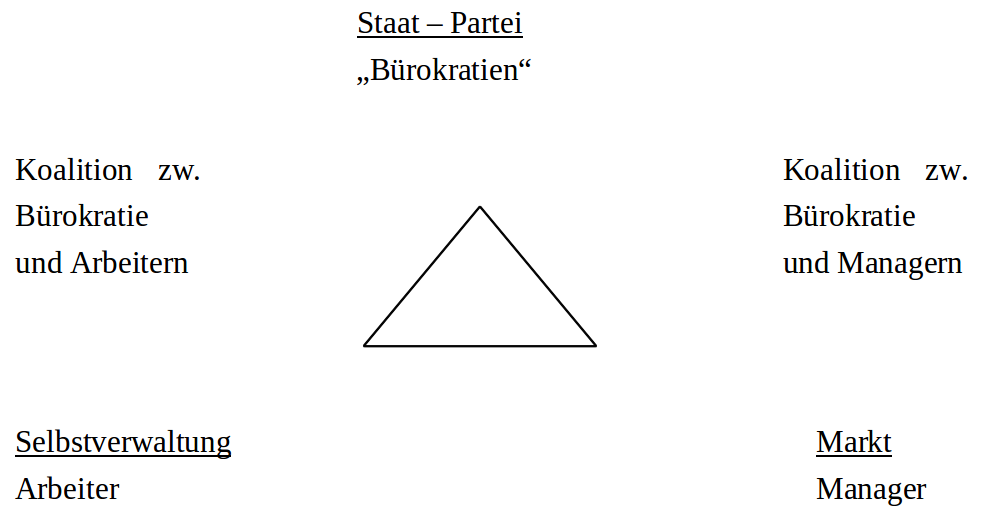
\includegraphics[width=4in]{Material/Parteienbuerokratie}\\
\vspace{0,5cm}
Quelle: nach \cite{mocnik}: 137.
\end{figure}

\subsubsection{Verwaltungsaufbau}

Die öffentliche Verwaltung in Jugoslawien entsprach zunächst der Verwaltung eines sozialistischen Staates mit Planungsfunktion. Die Staatsverfassung kannte keine klassische Gewaltenteilung, so dass Verwaltungsmaßnahmen nicht nur von den eigentlichen Verwaltungsorganen getroffen wurden, sondern auch von Gesetzgebungs- und Repräsentationsorganen. Dennoch wies die Verwaltung Jugoslawiens im Vergleich zu anderen sozialistischen Verwaltungen einige Besonderheiten auf. Seit Ende des Zweiten Weltkrieges waren vier Phasen (bis 1975) erkennbar.
\begin{enumerate}[label={\Roman*}:,align=left,  leftmargin=*]
\item  In der ersten Periode wurde das sowjetische Verwaltungskonzept nachgebildet, diese Periode ging formell 1952 zu Ende. Bis 1952 waren die staatliche Administration und der civil service stark zentralistisch und hierarchisch organisiert. Staatseigene Betriebe, die öffentliche Aufgaben wahrnahmen, wie Gesundheits- und Bildungseinrichtungen, hatten auch den Status von Verwaltungseinheiten (vgl. \cite{sevic}: 54). Während alle exekutiven und administrativen Kompetenzen beim Zentralstaat lagen, hatten die Republiken in ihrem Bereich Befugnisse, allerdings nur zur Ausführung zentralstaatlicher Gesetze.
\item Die Periode der Abwendung vom sowjetischen Vorbild, mit Abbau des demokratischen Zentralismus, Übergang von staatlichen Plänen zu gesellschaftlichen Plänen, Ausbau der Selbstverwaltung der Republiken, territorialer Verwaltungsdezentralisation. Mit einer Verfassungsänderung 1953 wurden diese Veränderungen umgesetzt (vgl. \cite{beckm90}: 52).
\item Der spezifische „Selbstverwaltungssozialismus“ ist in der Verfassung von 1963 verankert. Der zentralistische Parteiapparat diente als Gegengewicht zur föderalen Staatsstruktur (vgl. \cite{roggemann}: 258). Bis 1967 wurden Gesetze an die neue Verfassung angeglichen, auch das im Jahr 1957 erlassene Verwaltungsrecht musste angepasst werden. Die neue Verfassung hat den Begriff „Volksdemokratie“ durch den Begriff „sozialistisches Land“ ersetzt. Die Volkskomitees wurden zugunsten lokaler territorialen Einheiten ersetzt. Das wesentliche Organ wurden die Versammlungen, die ihre eigene Verwaltung und Räte bekamen (vgl. \cite{blago69}: 5). 
\item Die Periode mit neuem Verfassungskonzept sowie neuer Kompetenzabgrenzung. Seit 1967 wurden immer mehr Verwaltungskompetenzen auf die Teilrepubliken übertragen (vgl. \cite{grot}: 134). Im Jahr 1974 trat eine neue Verfassung in Kraft, die weitgehende Kompetenzen der Republiken und der Selbstverwaltungsrechte der unteren Verwaltungsebenen und gesellschaftlicher Gruppierungen festschrieb. Weiterhin sollten Wirtschaftsorganisationen direktere Mitspracherechte haben (vgl. \cite{beckm90}: 80ff.). 
\end{enumerate}

Es entstanden vier Ebenen der Verwaltung: 1. Die Föderation, 2. die Republiken, 3. die autonomen Provinzen und 4. die territorial-administrativen Einheiten (Gemeinden, Städte, Distrikte, Regionen). Distrikte und Städte hatten lokale Selbstverwaltungsfunktion, analog ihren Aufgaben im 19. Jh., waren aber gegenüber der lokalen Legislative verantwortlich und die zentralstaatliche Ebene konnte die unteren Ebenen der Administration anweisen. (vgl. \cite{sevic}: 47). Neben der neuen Verfassung für Jugoslawien 1974 verabschiedeten die sechs Republiken eigene Verfassungen mit genauen Aufgabenbeschreibungen und Kompetenzzuweisungen. Dabei wurde der Bundesstaat als „staatliche Gemeinschaft freiwillig vereinter Völker und ihrer sozialistischen Republiken“ (Art. 1 Verf. 1974) beschrieben. Die sozialistischen Republiken wurden ausdrücklich als Staaten verstanden mit dem Volk als Träger der Souveränität (Art. 3 \& 4 Verf. 1974). Gleichzeitig enthielt die Verfassung keinen eindeutigen Bezug auf eine jugoslawische Nation. Der Bund bearbeitete einige wesentliche ihm zugewiesene Bereiche, wie Auswärtige Beziehungen, Landesverteidigung und Staatssicherheit und war für die Aufrechterhaltung des einheitlichen Rechts- und Wirtschaftssystems verantwortlich. Die Republiken waren in allen anderen Belangen zuständig und auch für den Vollzug der Bundesgesetze, außer für Fälle, in denen ein Bundesorgan ermächtigt war. Den Bundesverwaltungsorganen stand für den Vollzug von Bundesgesetzen kein unbeschränktes Durchgriffsrecht zu, sondern sie hatten den föderativen Dienstweg über die entsprechenden Organe der Republiken einzuhalten (vgl. \cite{roggemann}: 286).\par
Die wesentlichen Ausführungsorgane hinsichtlich der Verwaltung waren die Gemeinden. Sie hatten grundsätzlich die Rechtsnormen der Gemeinden, der Republiken und autonomen Provinzen sowie des Bundes auszuführen. Weiterhin oblag ihnen die Durchführung des Verwaltungsverfahrens. Die Verwaltungsorgane der Republiken und autonomen Provinzen waren im Wesentlichen in einer Aufsichts- und Koordinierungsfunktion tätig. Die Ausführung durch die Gemeindeebene und die Aufsichtsfunktion durch die Ebene der Republiken und autonomen Provinzen haben viel Kritik auf sich gezogen und wurden von der Bundesebene als nicht effizient dargestellt (vgl. \cite{beckm90}: 209ff.). Die komplizierte Machtbalance zwischen der Föderation und den Republiken und autonomen Provinzen, ab 1974 angereichert um die verstärkten Selbstorganisationsbefugnisse, führte zu einer zunehmenden Lähmung des Staatsapparates. Nach Einschätzung von zeitgenössischen Beobachtern wendeten die Republiken und Gemeinden eine Taktik der „Nichtausführung“ von Gesetzen an. „Es ist vielmehr wesentlich bequemer, auf der Bundesebene für diese Maßnahme einzutreten – mit dem geheimen Vorbehalt, sie nicht auszuführen und so kurzfristige egoistische Ziele zu verfolgen. Ein weiterer Grund für den mangelhaften Gesetzesvollzug liegt in vielen Gesetzen selber: sie sind zum Teil überfrachtet mit Absichtserklärungen, unnötigen Wiederholungen und zu allgemein gefasst, so dass es nahezu unmöglich ist, ihnen eine klare Verhaltensnorm zu entnehmen“ (vgl. \cite{beckm90}: 224). Elemente der französischen Verwaltungstradition, die im 19. Jh. Einfluss auf Slowenien und Teile Kroatiens hatten, bestanden auch im sozialistischen Jugoslawien weiter.

\subsubsection{Vom Beamten zum Staatsbediensteten}

Bis zum Jahr 1946 war das 1931 für das Königreich Jugoslawien erlassene Beamtengesetz in Kraft, das alle Grundelemente, die für den Beamtenstatus typisch sind, beinhaltete. Mit einem neuen Gesetz wurde 1946 den staatlichen Bediensteten das hoheitliche Entscheidungsrecht entzogen. Sie waren nun weder Träger der Staatsgewalt, noch konnten sie diese ausüben. Dieses Recht kam nur noch den gewählten Funktionären zu. Der Begriff Staatsbediensteter wurde geprägt, worunter umfassende Verwaltungs- und Facharbeit unter Anleitung der gewählten Funktionäre zu verstehen war. Staatsbedienstete übten also wesentlich umfassendere Aufgaben aus als Beamte, aber ohne deren Kompetenzen. Bis 1957 war diese Rechtsordnung in Kraft (vgl. \cite{vavpetic}: 108).\par
1957 ersetzte das Bundesgesetz über die Staatsbediensteten das gleichnamige Gesetz von 1946. Beide Gesetze gingen von einer besonderen Rechtsstellung der Staatsbediensteten aufgrund ihrer besonderen Aufgaben aus. Die unterschiedlichen Regelungen für Staatsbedienstete und das allgemeine Arbeitsrecht wurden in der neuen Verfassung von 1963 aufgegeben (vgl. \cite{sevic}: 55). So verlor das Gesetz über die öffentlichen Bediensteten 1965 seine Gültigkeit. Das neue Gesetz über die Arbeitsverhältnisse enthielt den Begriff öffentlicher Bediensteter nicht mehr. Man sprach nur noch vom Arbeiter, unterschieden nach Hand- oder Kopfarbeiter. Für alle galten die gleichen Bestimmungen. \par
Nun wurde das gleiche Recht, das Arbeitsrecht, auf alle öffentlich Bediensteten angewandt (vgl. \cite{markic}: 12). Die Leistungen, die von diesen öffentlichen Bediensteten erbracht wurden, kann man im Sinne eines „public service“ definieren. Die jugoslawische Besonderheit war, dass viele Organisationen nicht direkt dem Bundesstaat unterstanden, sondern im Selbstverwaltungssystem als Gesellschaftsorganisationen bestanden (z.B. Gesundheits-, Wissenschafts- oder Bildungseinrichtungen) (vgl. \cite{vavpetic}: 113).

\subsubsection{Verwaltungsgerichtsbarkeit }

Nach dem Zweiten Weltkrieg wurde 1952 wieder eine generelle administrativ-juristische Kontrolle der öffentlichen Verwaltung eingeführt. Damit war Jugoslawien das einzige kommunistische Land, das einen gerichtlichen Verwaltungsrechtsschutz vorsah. Die Verfassung Jugoslawiens von 1974 delegierte die Organisation der Justiz an die Republiken. Auseinandersetzungen über administrative Entscheidungen wurden meist von den höchsten Gerichten der föderalen Strukturen (Republiken und Autonomen Provinzen) entschieden (vgl. \cite{roggemann}: 317). Der meist letztinstanzlichen gerichtlichen Überprüfung musste ein behördliches Widerspruchsverfahren vorangegangen sein. Für die Anfechtung von Akten der Bundesverwaltungsorgane war das Bundesgericht zuständig. Wirtschaftsgerichte waren für die Anfechtung bestimmter Akte der Finanzverwaltung zuständig sowie Militärgerichte für Maßnahmen der Militärbehörden (vgl. \cite{beckm90}: 234). Rechtsstreite in Fragen des Dienstrechts der Verwaltungsangestellten wurden von den Arbeitsgerichten entschieden. Kontrolle der öffentlichen Verwaltung wurde durch eine Staatliche Kontrollkommission ausgeübt, die allerdings als unzulänglich eingeschätzt wurde. Während die individuelle Verfassungsbeschwerde 1974 in der Verfassung abgeschafft wurde, wurde jetzt den Gerichten diese Grundrechtskompetenz zugewiesen, die sie im Verwaltungsstreitverfahren wahrnehmen sollten (vgl. \cite{roggemann}: 318).

\subsubsection{Die Staatskrise Jugoslawiens}

Die Verfassungsreform von 1974 hat die Dezentralisierungstendenzen im jugoslawischen Staat fortgesetzt, womit Nationalitätenkonflikte innerhalb des Landes kanalisiert und aufgefangen werden sollten (vgl. \cite{roggemann}: 282). Gleichzeitig änderte sich an den wirtschaftlichen Disparitäten zwischen den Republiken und Provinzen im Laufe der Zeit wenig. Unterentwickelte, meist stark agrarisch geprägte Regionen, insbesondere Kosovo, Mazedonien und auch Montenegro konnten kaum aufholen und wurden wirtschaftlich zunehmend „abgehängt“. Auch ein Ausgleichsfonds, der Gelder von den wirtschaftlich besser gestellten Republiken (vor allem Slowenien und Kroatien, die 45\% der Mittel des Fonds bereitstellten) in die randständigen Gebiete umverteilen sollte, zeigte keine nachhaltige Wirkung (vgl. \cite{ramet}: 380).\par
Im Zuge der sich zuspitzenden Staatskrise nach Titos Tod 1980 erstarkten die Teilstaaten auch aufgrund des zentralstaatlichen Machtvakuums und übernahmen Machtbefugnisse der Zentralregierung. Sowohl eine 1983 eingeleitete Wirtschaftsreform als auch die später einsetzende Reform des politischen Systems wurden in langwierigen Prozessen von eigens eingesetzten Kommissionen in mehrjähriger Arbeit mit Abschlussberichten vorbereitet. Um zunehmende öffentliche Kritik aufzufangen, wurde 1982 eine Analyse des politischen Systems in Jugoslawien im Auftrag des Kongresses des Bundes der Kommunisten Jugoslawiens (BdKJ) erstellt. Nach umfassenden Beratungen wurden die Ergebnisse der Bevölkerung vorgestellt als Broschüre „Kritische Analyse“ in einer Sonderbeilage zu den überregionalen Tageszeitungen im Januar 1986. Einer der Ausgangspunkte für die Arbeit an der „Kritischen Analyse“ war die Lähmung des politischen Systems durch das faktische Vetorecht der Republiken und Provinzen bei allen Gesetzesinitiativen, das dazu führte, dass kaum noch Entscheidungen getroffen werden konnten (vgl. \cite{reuter}: 399).\par
Die sich zuspitzenden Schwierigkeiten in Jugoslawien schrieb 1985 der Präsidiumsvorsitzende des ZK des BdKJ auch der Staatsstruktur zu, welche die egoistische Verfolgung von Eigeninteressen der Teilrepubliken ermöglichte. „Der polyzentristische Etatismus ist die Hauptursache für [unsere] Wirtschaftskrise, technologische Stagnation und unsere finanzielle Abhängigkeit vom Ausland. […] Im vergangenen und im laufenden Jahr haben wir gravierende Probleme bei der Entscheidungsfindung im Bund, vor allem bei der Kompromissfindung zwischen den Republiken und Provinzen miterlebt. […] Es ist unannehmbar, dass Delegationen und oft auch den Abgeordneten in den Räten des Parlaments der SFRJ Anweisungen gegeben werden, wie lange sie bestimmte Standpunkte diskutieren sollen, wann und bis zu welchem Grad sie nachgeben sollen, um auch die belanglosesten Interessen ihrer Republiken und Provinzen zu befriedigen“ (Tanjug, 22.9.1985, zit. in:  \cite{ramet}: 449).\par
Im Zuge wirtschaftlicher Schwierigkeiten mit einer zunehmenden Schuldenkrise zerbrach Jugoslawien nicht zuletzt in Folge der politischen Umwälzungen von 1989. Lampe benennt als allgemeine Ursachen der jugoslawischen Krise am Ende der 1980er Jahre:
\begin{itemize} \itemsep1pt \parskip0pt \parsep0pt
\item Veränderung des internationalen Umfelds (Epochenwandel 1989/91) – Der Westen verliert das Interesse an einem eigenständigen Jugoslawien – Ende der „Alimentation“ Jugoslawiens;
\item allgemeine Diskreditierung aller Formen von Ein-Parteiensystemen;
\item innerwirtschaftliche Probleme (notwendige Investitionsanstrengungen zugunsten von Lohnsteigerungen eingeschränkt) (vgl. \cite{lampe}: 329).
\end{itemize}
Für den weiteren Fortgang der Untersuchung ist wichtig festzuhalten, dass sich Jugoslawien stark von der extrem zentralistisch ausgerichteten Verfasstheit in den ehemals kommunistischen Staaten Osteuropas unterschied. In Jugoslawien bestand nach dem Zweiten Weltkrieg die Tradition kontinentaleuropäischer Verwaltungsstrukturen zunächst fort, bevor diese im neuen sozialistischen Staat sukzessive umgebaut wurden. Das anfänglich noch bestehende System des Berufsbeamtentums wurde umgewandelt und ab den 1970er Jahren arbeitsrechtlich nicht mehr unterschieden zwischen Personen, die staatliche Aufgaben wahrnahmen und Arbeitern sowie anderen Angestellten. Im Gegensatz zu diesem Abbau des Berufsbeamtentums hatte das Prinzip der Überprüfbarkeit von Verwaltungshandeln, zumindest nominell, in Jugoslawien Bestand. Weiteres Kennzeichen der Entwicklung in Jugoslawien war die starke Zunahme der Kompetenzen der Republiken, die einherging mit der Abnahme der Gestaltungsmacht und Zuständigkeit der Zentralregierung. Dies fand seinen Höhepunkt in der Verabschiedung der Verfassung von 1974. Ab diesem Zeitpunkt beschleunigte sich die Abnahme der staatlichen Einheit mit dem weiteren Erstarken der Republiken, die den Einfluss der Zentralregierung zu minimieren versuchten. Allerdings ist zu beachten, dass durch den Zugriff der Partei auf die Administration aller Ebenen nicht von einer „echten“ Dezentralisierung gesprochen werden kann. Das endgültige Auseinanderfallen des Staates begann in Folge der politischen Wende in Osteuropa 1989 und die Neugründung von Staaten auf der Basis der bisherigen Republiken wurde begleitet von ethnischen Abgrenzungskonflikten. \par


\subsection{Historische Verwaltung Albaniens }
Zur Darstellung der Entwicklung in Albanien kann auf die Masterarbeit der Autorin zum Thema „Dezentralisierung des öffentlichen Sektors in Albanien im Spannungsfeld von Verwaltungsmodernisierung und EU-Annäherung“ zurückgegriffen werden, die im Sommersemester 2007 im Studiengang „Öffentliches Management“ zur Erlangung des Grades „Master of Public Administration“ (MPA) im Fachbereich „Wirtschaftswissenschaften“ der Universität Kassel vorgelegt wurde. Auszüge aus der Masterarbeit wurden in der vorliegenden Arbeit eingefügt und die entsprechenden Kapitel mit „Vollmer 2007“ kenntlich gemacht.\par
Nach dem chronologischen Ablauf wird die Entwicklung Albaniens in „Vor-osmanische und osmanische Zeit“ sowie weitere Unterabschnitte zu den einzelnen historischen Stationen unterschieden.
\subsubsection[Vor-osmanische und osmanische Zeit]{Vor-osmanische und osmanische Zeit\footnote{Vgl. \cite{vollmer07}: 7ff.}}
Das heutige geografische Albanien befand sich von der Antike bis zur osmanischen Eroberung im 14. Jahrhundert unter römischer, byzantinischer, später serbischer und bulgarischer, zeitweise auch normannischer und neapolitanischer Herrschaft. Bis zur Staatsgründung 2912 war das Gebiet fünfhundert Jahre lang Bestandteil des Osmanischen Reichs (vgl. \cite{winnifrith}: 16).\par
Die türkische Besatzung hatte akzeptiert, dass die Nordalbaner der Berge keine Steuern zahlten und räumte ihnen im Rahmen ihrer ungeschriebenen Gesetze, die sie seit Jahrhunderten befolgten, Selbstverwaltung ein. Es gab keine Straßen in das unwegsame Gebiet und die erste Straßenverbindung wurde unter der österreichischen Militärverwaltung 1916 von Shkodra nach Durres gebaut (vgl. \cite{hasluk}: 9). In den unzugänglichen Bergregionen wurde eine Autonomieregelung mit Verbindungsmännern zur zentralen Regierung und Eigenverantwortung für regionale administrative Aufgaben angewandt. Die Stammes- und Clanstrukturen blieben in diesen Landesteilen bestimmend für die Sozialisation. Interessengegensätze innerhalb und zwischen den Stammesgruppen und Familien unterlagen nach wie vor der Reglung durch das Gewohnheitsrecht. Eine zentrale politische Autorität konnte die osmanische Herrschaft in diesen Gebieten nicht durchsetzen (vgl. \cite{hens99}: 74).\par
Gegen Ende des 17. Jh.s führte eine Änderung in der osmanischen Finanzpolitik zu einem Islamisierungsschub in Albanien. Während bislang die Steuern für Nichtmuslime moderat waren und von der gesamten Gemeinde eingebracht wurden, erhob man nun Steuern auf individueller Basis. Die einsetzende Islamisierung albanischer Christen war dennoch oft eine formelle und die alten Stammesbräuche lebten weiter (vgl. Zhelyakova, 2002: 243). Mit dem zunehmenden Machtverlust des Osmanischen Reiches im 18. Jahrhundert, setzten auch in Albanien Sezessionsbestrebungen ein. Im Norden gelang es dem Provinzstatthalter von Shkoder eigene Handelsbeziehungen und diplomatische Beziehungen zu europäischen Mächten aufzubauen (vgl. \cite{vickers}: 18f).\par
Mit umfangreichen Reformen versuchten die osmanischen Machthaber ab den 30er Jahren des 19. Jahrhundert dem drohenden Zerfall des Imperiums entgegenzuwirken. Nichtmuslime wurden mit Muslimen gleichgestellt, ein neues Justizsystem wurde eingeführt und das Steuersystem neu organisiert. Die Reformen hatten Auswirkungen vor allem in Flachlandgebieten, wo Formen einer modernen Verwaltungsführung entstanden. In den Bergregionen und aufgrund von fehlender Infrastruktur in unzugänglichen Gebieten stellten nach wie vor die Familie und der Clan den Hauptbezugspunkt der persönlichen und kollektiven Identität (vgl. \cite{kaser}: 292).\par
Nach einem Aufstand erkannte die türkische Herrschaft Albanien als autonome Administration mit den vier Provinzen Scutari, Kosovo, Monastir und Janina an und es wurden lokale Verwalter eingesetzt. Schulen konnten nun in albanischer Sprache unterrichten. Dieser Aufstieg eines autonomen Albanien kollidierte mit Gebietsansprüchen Serbiens auf das Kosovo und Montenegros auf Scutari (Shkodra), die auch die europäischen Mächte auf den Plan riefen. In einem Krieg der Balkanstaaten 1912 gegen die Türkei wurden albanische Gebiete von anderen Nachbarländern (Montenegro, Serbien und Griechenland) besetzt. Die Interessen Italiens und Österreich-Ungarns in der Region und der Antagonismus mit Russland, das Serbien unterstützte, ließen einen internationalen Konflikt am Horizont aufscheinen (vgl. \cite{chek}: 63).\par
 In der folgenden Landkarte ist ersichtlich, dass zwar Gebiete der späteren Staaten Mazedonien
und Albanien um 1912 noch unter Einfluss des Osmanischen Reiches waren,
Montenegro dagegen nicht.
\begin{figure}[H]
  \centering
\setlength\belowcaptionskip{10pt}
  \caption{Einfluss des Osmanischen Reiches im Balkan 1912}
  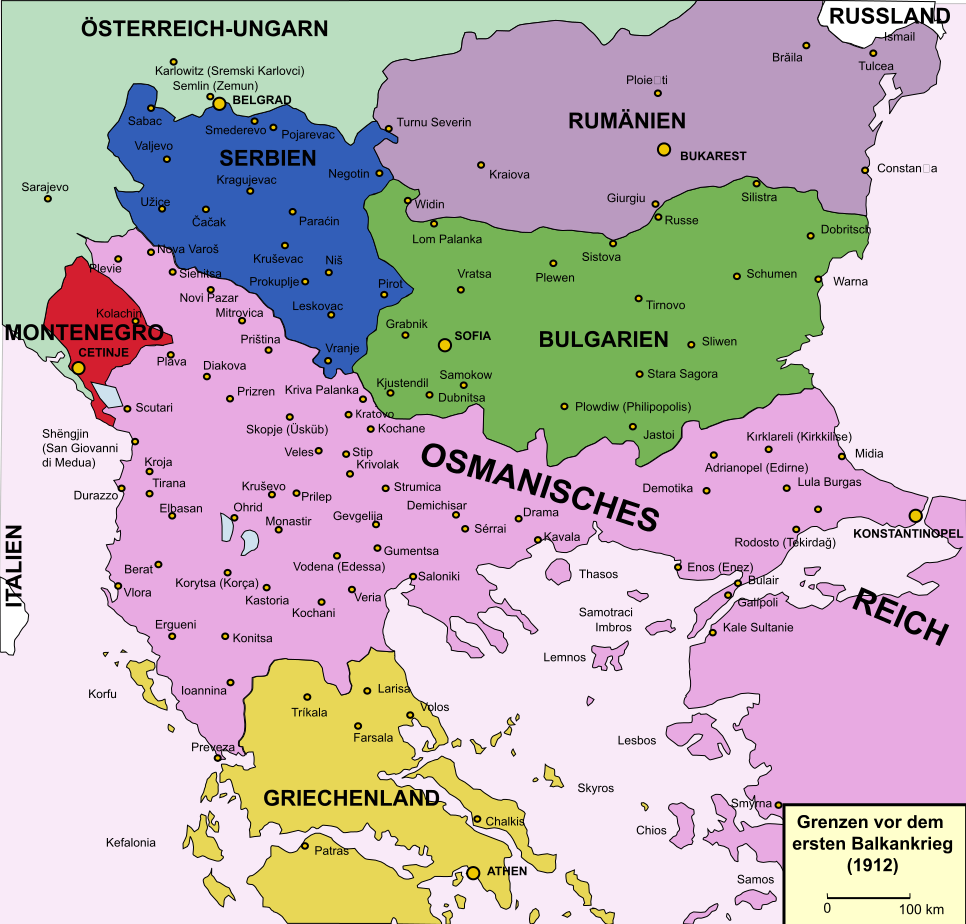
\includegraphics[width=5in]{Material/Balkan_1912}\\
\vspace{10pt}
Quelle: http://de.wikipedia.org/w/index.php?title=Datei:Balkan\_1912.svg\\ (Aufgerufen: 22.8.2012).
\end{figure}

\subsubsection[Staatsgründung 1912 ]{Staatsgründung 1912\footnote{Vgl. Vollmer 2007: 10.}}

Im Vertrag von Bukarest, mit dem der Zweite Balkankrieg zu Ende ging, legten die führenden Mächte die Grenzen Albaniens fest. Die Gründung des albanischen Nationalstaates am 28. November 1912 nach fast 500 Jahren unter osmanischer Herrschaft war im Interesse der Großmächte. Angesichts des Machtverlustes des Osmanischen Reiches sollte ein Gegengewicht geschaffen werden gegen eine slawische Expansion (vgl. \cite{biber}: 18). In der Beilegung des Konfliktes der Balkanländer und ihrer jeweiligen Verbündeten durch eine internationale Konferenz wurde erstmals ein unabhängiges Albanien anerkannt. Die Abtrennung von Albanern bewohnter Gebiete wurde beschlossen\footnote{Von Albanern bewohnte Gebiete, die von Serbien (Kosovo), Montenegro (ein Gebiet am Mittelmeer) und Griechenland (Cameria) besetzt waren, wurden den Besatzern zugesprochen.} und Albanien sollte von einem Prinzen\footnote{Der Deutsche Verwalter, Prinz Wilhelm zu Wied verließ aufgrund lokaler Widerstände bei Ausbruch des ersten Weltkriegs das Land (\cite{biber}: 18). }, auf den sich die europäischen Mächte einigten, regiert werden. Alle sechs europäischen Mächte (Österreich-Ungarn, Deutschland, Italien, Russland, Frankreich, Großbritannien) sollten in einer internationalen Kontrollkommission für Albanien präsent sein. Die Kontrollkommission hatte die Aufgabe, die Ausgaben überprüfen, der Regierung bei der Administration des Landes zu assistieren und einzuschreiten bei juristischen Übertretungen der albanischen Regierung. Die Kommission war einflussreich aber uneffektiv, da ihre Mitglieder hauptsächlich die Interessen ihrer Entsendungsregierungen vertraten, die sich zum Teil diametral gegenüberstanden (vgl. \cite{chek}: 127).\par
Im Anschluss an die Staatsgründung wurde das politische Geschehen dominiert von dem Wunsch nach Wiedergewinnung der verlorenen Gebiete und der Sorge um die instabile Lage auf dem Balkan. Der Aufbau und die Modernisierung des Staatswesens kamen nicht voran (vgl. \cite{hens99}: 82).
\subsubsection{K.u.k. Militärverwaltung 1916-1918}

Während des Ersten Weltkrieges befanden sich Nord- und Mittelalbanien von 1916 bis 1918 unter österreichisch-ungarischer Militärverwaltung. Wie der Entwicklungsstand des besetzten Landes eingeschätzt wurde, wird in einer geheimen Note des österreichisch-ungarischen Generalstabes exemplarisch deutlich: „Das albanische Volkskonglomerat bedarf einer Generationen dauernden kultivierenden und erzieherischen Tätigkeit mit straffer Hand im Rahmen unserer Monarchie, um zu jener Blüte zu gelangen, zu der es vom wirtschaftlichen Standpunkt fähig wäre.“\footnote{HHSTA, PA I, Karton 1001, Geheime Note des k.u.k. Chefs des Generalstabes, 28.Mai 1916, OP.No.25.492.} Zum Zustand der Administration wird ebenfalls Stellung genommen: „Die lang anhaltende türkische Herrschaft ist zweifellos die Hauptträgerin der Schuld, sie hat das Land nicht gedeihen lassen, das Volk aber verdorben. Fast methodisch wurde Albanien von allen äußeren kulturellen Einflüssen ferngehalten [...] die Regierung wollte einfach die primitiven Verhältnisse, weil sie glaubte, auf diese Weise am wenigsten Scherereien zu haben. Freiheiten ließ sie genug, sie schuf Privilegien, hob fast keine Staatssteuern ein etc., lange ging die Sache so hin, endlich drangen aber doch andere, moderne, wenn auch unausgegorene Ideen ins Land, es kamen die Balkanwirren und jetzt erscheinen kaleidoskopartig die verschiedenen Verwaltungen und Regierungen: die des Ismail, die internationale, die Wiedsche, jene Essads, von Serben und Montenegrinern (in Teilen), endlich die österreich-ungarische.“\footnote{HHSTA, PA I, Nr. 1001, Geheime Note des k.u.k. Chefs des Generalstabes, 28.Mai 1916, OP.No.25.492, Beilage 1.} Anders als in Montenegro, wo von der österreichisch-ungarischen Besatzungsmacht eine funktionierende Verwaltung vorgefunden wurde, gab es in Albanien allenfalls archaische Verwaltungsstrukturen.\par
Aus einem militärischen Lagebericht wird die Problematik einer zu ambitionierten Verwaltungsreform seitens der Besatzer selbstkritisch angemerkt: „Bezüglich der Behandlung der albanischen Verwaltungsangelegenheiten wird vorläufig an dem Grundsatz festgehalten, nicht allzu reformierend aufzutreten, da ansonsten die alte eingelebte, wenn auch schwerfällige und verzopfte, aber doch zur Not entsprechende Regierungsform genommen und wegen Mangel an geeigneten Personen keine sofort brauchbare neue gegeben wird. Aus diesem Grund werden im Allgemeinen die alten türkischen Gesetze und Vorschriften beibehalten und nur die notwendigsten Änderungen vorgenommen.“\footnote{HHSTA, PA I, Karton 1001, Lagebericht Feldpostamt 140, 9.September 1916, Trollmann, k.u.k. XIX Korpskommando, E.V. Nr. 962/IX.}\par
In der Folge waren erhebliche Fortschritte in der Reformierung bzw. dem Aufbau der Zivilverwaltung zu verzeichnen, mit Ausgestaltung der verschiedenen Zweige der Administration und der Einteilung aller Landesangestellten in bestimmte Rangklassen mit festgelegtem Gehaltsschema. Es wurde eine Dienstpragmatik erlassen sowie die Arbeitszeit und Öffnungszeiten der Ämter festgelegt.\footnote{HHSTA, PA I, Karton 1006, Z. 56/P.Kral, Shkodra, 5. April 1917. } Weiterhin wurden Verfahren vor den Zivilgerichten kodifiziert, basierend auf türkischem Recht. Im Sommer 1916 wurde ein Gerichtssystem eingerichtet mit Friedensgerichten für kleinere Zivil- und Handelsstreitigkeiten, Berufungsgerichten, und für größere Streitigkeiten in vier Städten und dem Appellationsgericht in Shkodra. In den Jahren 1916 und 1918 wurde eine Volks- und Viehzählung durchgeführt, die offenbar mit einigem Aufwand verbunden war. „Mit Rücksicht darauf, dass in diesem Lande, speziell in den schwer zugänglichen Gebirgsdistrikten eine derartige Zählung noch nie stattgefunden hatte, muss die einschlägige Aktion, die verhältnismäßig gut gelungen ist, als ein bedeutungsvoller Fortschritt in der Verwaltung Albaniens bezeichnet werden.“\footnote{HHSTA, PA I, Karton 1006, Z. 184/P.Kral, Shkodra, 16. November 1916.} Im Januar 1918 wurden die Erbschaftsangelegenheiten der Christen von den Sheriatsgerichten an die Zivilgerichte verwiesen und ein eigenes Erbrecht wurde in Auftrag gegeben. Weiterhin wurde die Neuorganisation des Schulwesens in einer Weise durchgeführt, die „durchaus modernen Anforderungen standhalten konnte und in gleicher Weise auf bodenständige Faktoren Rücksicht nahm“ (\cite{schwanke}: 177). Während der österreichisch-ungarischen Besatzungszeit sind umfangreiche Arbeiten am Straßennetz erfolgt und ca. 840 km Straßen und zahlreiche Brücken gebaut sowie Telefon- und Telegrafenverbindungen eingerichtet worden. Während diese vor allem militärischen Zwecken dienten, haben sie doch zu einer nachhaltigen Verbesserung der Infrastruktur beigetragen.\par
Die Organisation des Steuerwesens in der Okkupationszeit konzentrierte sich darauf, die alten Gesetze und Gewohnheiten beizubehalten und diese erst allmählich zu modernisieren und auf Gebiete auszudehnen, die zu türkischer Zeit keine oder nur unter großen Schwierigkeiten Steuern gezahlt hatten. So wurde die Zehntsteuer beibehalten und auch die Gebiete der Ebene um Shkodra erstmals einbezogen, während in der Gebirgsregion aufgrund von Armut und schlechter Ernte eine kumulative Kopfsteuer eingezogen wurde.\footnote{Vgl. HHSTA, PA I, Karton 1006, Nr. 163/P.Kral, Shkodra, 30. Juni 1918.}\par
Die Früchte dieser Arbeit zur Modernisierung der Verwaltung konnte die Monarchie am Ende des Weltkrieges nicht mehr ernten. Umso mehr baute der 1921 neu erstandene albanische Staat seine Verwaltung auf den von der k.u.k Militärverwaltung geleisteten Vorarbeiten auf. „Ohne die von Österreich-Ungarn geleistete Pionierarbeit auf dem Verwaltungssektor wäre eine beinahe dreijährige Verwaltung mit ihrer lang nachhaltigen Wirkung über den Ersten Weltkrieg hinaus nicht möglich gewesen“ (\cite{schwanke}: 89). Politischer Hintergedanke dieser Aufbauarbeit war sicherlich auch das Ziel, eine günstige Ausgangsstellung in Bezug auf politische und wirtschaftliche Beziehungen mit dem strategisch günstig gelegenen Albanien zu schaffen.

\subsubsection[Zwischenkriegszeit]{Zwischenkriegszeit\footnote{Vgl. \cite{vollmer07}: 11ff.}}

In den frühen 20er Jahren war Albanien zwischen zwei grundlegend gegensätzlichen Kräften aufgeteilt: Einerseits konservativen Lokalfürsten, die Albanien nach den alten osmanischen Regeln beherrschen wollten. Auf der anderen Seite fanden sich liberale Intellektuelle, demokratische Politiker und fortschrittliche Handeltreibende, die sich unter der Führung eines südalbanischen Bischofs der orthodoxen Kirche nach Westen orientierten.\par
In den 1920er Jahren erlangte ein lokaler Führer aus dem Norden mittels eines militärischen Coup die Macht und etablierte 1928 eine Monarchie. Eine Reform des Landes fand nicht statt und trotz immenser Nahrungsmittelimporte verließen tausende Albaner ihr Land auf der Suche nach einem besseren Leben. Es bestand zwar eine lokale Verwaltung, doch die von der Zentralregierung ernannten Präfekten übten politische Kontrolle über die Regionen und damit über die Distrikte und Kommunen aus. Lediglich die Distriktversammlungen (insgesamt 36 Distrikte) waren gewählt, alle anderen Funktionen inklusive der Bürgermeister wurden ernannt. In den Gebieten des Nordens fand weiterhin keine Eingliederung in staatliche Strukturen statt, es wurden keine Steuern gezahlt und Verordnungen des Staates konnten nur mit Zustimmung der lokalen Führer durchgesetzt werden (vgl. \cite{biber}: 19).\par
Die Unabhängigkeit Albaniens 1912 brachte keine nennenswerten Fortschritte für das wenig entwickelte Land. Traditionelle Gesellschaftsstrukturen und die schwierige ökonomische Situation behinderten eine Modernisierung. Albanien war fast vollständig von Wareneinfuhren und Hilfslieferungen abhängig, die vor allem von Italien zur Verfügung gestellt wurden. Italien stellte auch Anleihen und Investitionen zur Verfügung, was zu einem quasi-kolonialen Status führte. Nach Beginn des Zweiten Weltkrieges annektierte das faschistische Italien 1939 Albanien (vgl. \cite{fisch84}: 283).
\par
Zusammenfassend wird deutlich, dass einer Modernisierung des Staatswesens in Albanien historisch betrachtet mehrere Entwicklungen entgegenstanden. Zunächst führte die Jahrhunderte dauernde osmanische Herrschaft zur Abschottung des Landes gegen kontinentaleuropäische Einflüsse. Auch die Isolation der Bewohner in den zahlreichen Bergregionen des Landes mit Gewohnheitsrecht und traditionalen Vergesellschaftungsformen wirkte sich aus. Besonders im Norden des Landes waren bis Ende des Zweiten Weltkrieges praktisch alle Versuche zu einer Modernisierung der Verwaltung ergebnislos verlaufen. Die zweijährige Zeit der k. u. k. Militärverwaltung in der nördlichen Hälfte von Albanien während des Ersten Weltkrieges kann dennoch als eine Zeit moderner Einflüsse auch in verwaltungstechnischer Hinsicht angesehen werden, auch wenn diese Einflüsse regional begrenzt waren.\par
Die kurze Phase Albaniens als unabhängiger Staat fiel in die Zeit zwischen beiden Weltkriegen und führte zu weiteren Besatzungen und schließlich zur Annexion durch das faschistische Italien. Aufgrund äußerer Bedrohungen und fehlender Erfahrungen der Administratoren sind auch in dieser Phase keine effektiven und umfassenden Neuerungen in der Verwaltungsstruktur des Landes durchgeführt worden. Nach dem Zweiten Weltkrieg etablierte sich in Albanien ein kommunistischer Staat mit spezifischen Auswirkungen auf die Verwaltungsentwicklung, die im Folgenden skizzenhaft dargestellt werden.
\subsubsection[Das kommunistische Albanien]{Das kommunistische Albanien\footnote{Vgl. \cite{vollmer07}: 14ff.}}

Im Widerstand gegen die Besatzung durch zunächst Italien und dann Deutschland während des Zweiten Weltkrieges setzte sich die kommunistisch orientierte Partisanenbewegung durch. Eine kommunistische Partei wurde in Albanien 1941 gegründet und 1944 eine Verfassung verkündet.\footnote{Eine direkte Kopie der jugoslawischen Verfassung.} Im Dezember 1945 fanden Wahlen statt, in denen fast ausschließlich Kandidaten der Kommunistischen Partei angetreten waren. Die Partei erhielt 93\% der Stimmen und die Volksrepublik mit Enver Hoxha an der Spitze wurde ausgerufen. Verbliebene Kritiker der Überführung Albaniens in einen kommunistischen Staat wurden umgebracht, vertrieben oder interniert (vgl. \cite{vickers}: 164).\par
Das Ziel der Verstaatlichung des Agrarsektors war Mitte der 70er Jahre weitestgehend erreicht, wobei auch erstmals auch die Bergregionen im Norden erfasst wurden. Die Industrialisierung des Landes wurde nach dem Ende des Krieges mit Hochdruck betrieben, wobei der Ausbau der Industrieproduktion stark von ausländischen Geldern und Kooperationen abhängig war.\footnote{Hauptsächlich Jugoslawien, Sowjetunion, COMECON und China.} Der Rückgang der selbstständigen Betriebe und die massive Industrialisierung mit Staatsbetrieben führten dazu, dass der Staat zum Hauptarbeitgeber wurde (vgl. \cite{hens99}: 89). Bürokratisierung auch einfacher Aufgaben und Bestechlichkeit des Personals waren während des kommunistischen Regimes Kennzeichen staatlicher Herrschaftsausübung. Der Zugang zu allen attraktiven Führungs- und Entscheidungspositionen wurde von der Partei reguliert. Die in allen sozialistischen und kommunistischen Regimen starken personellen und ideologischen Loyalitätsbedingungen trafen in Albanien auf die durchaus ähnlichen Muster der Clan- und Stammesstrukturen, die über Jahrhunderte das Leben in der traditional geprägten Gesellschaft bestimmt hatten (vgl. \cite{vickers}: 189). Auch gegen die Gegner des Systems wurde die Tradition der Loyalität zum erweiterten Familienkreis instrumentalisiert. In Ungnade gefallene Funktionsträger wurden oft mitsamt ihrer Familien in Internierungslager verbannt. Ähnlich anderen kommunistischen Ländern, wurde in Albanien die öffentliche Verwaltung stark zentralistisch und vertikal ausgerichtet. Eine lokale Ebene bestand zwar und wurde durch Wahlen alle vier Jahre bestimmt, doch hatte diese Ebene keinerlei eigenständige Politikgestaltungsbefugnis. Das Budget, mit Instruktionen zu seiner Verwendung, wurde zentral zur Verfügung gestellt. 36 Distrikträte waren zuständig für die Überwachung der Einhaltung der Produktionspläne der industriellen und landwirtschaftlichen Staatsbetriebe im jeweiligen Distrikt (vgl. \cite{hoxha}: 5). Die von den Kommunisten verfolgte Modernisierung der Gesellschaft gelang nur oberflächlich.

\subsubsection[Der Weg in die außenpolitische Isolation]{Der Weg in die außenpolitische Isolation\footnote{\cite{vollmer07}: 15ff.}}

Außenpolitisch beschritt Albanien einen Weg, der zu einem gewissen Teil mit der Verhaftung in vormodernen Traditionen erklärt werden kann. Dabei folgte auf eine Zeit der Freund-Feind-Konstellation mit jeweils einem starken Verbündeten, ab Ende der 1970er Jahre eine Zeit der zunehmenden und selbst gewählten außenpolitischen Isolation. Von 1944-48 war es vor allem Jugoslawien, das den albanischen Interessen als eigenständiger Staat bei den Vereinten Nationen Nachdruck verlieh und umfangreiche finanzielle Hilfe für den Aufbau des Staatswesens zur Verfügung stellte. Auf der anderen Seite war Jugoslawien bestrebt, Albanien ökonomisch sehr eng an sich zu binden, woraus die Befürchtung entstand, Jugoslawien wolle die politische Kontrolle über Albanien erlangen. 1948 kam es daher zum Bruch mit Jugoslawien gefolgt von einer Hinwendung zur Sowjetunion (vgl. \cite{odonnell}: 29ff). Die außenpolitischen Beziehungen zur Sowjetunion stärkten Albanien, das nun eine Weltmacht zum Verbündeten hatte. Allerdings kühlten sich die Beziehungen nach Stalins Tod 1953 deutlich ab. Zum endgültigen Abbruch der Beziehungen zur Sowjetunion kam es 1961.\par
Ab Mitte der 1950er Jahre trat China in Vordergrund und stellte ab 1957 Finanzhilfe für Albanien zur Verfügung. In der Folgezeit konzentrierte sich Albanien auf die ökonomische und militärische Unterstützung durch China, bis auch diese Allianz 1978 von Albanien aufgekündigt wurde. Nach dem Bruch mit der Volksrepublik China bis zum Tode Enver Hoxhas 1985 war Albanien außenpolitisch vollständig isoliert. Nach Beginn der Systemwechsel in Osteuropa verlor die kommunistische Partei in Albanien Ende 1990 ihr Monopol und die ersten freien Wahlen fanden am 31.3.1991 statt (vgl. \cite{ammann}: 486). Der Beitritt zur OSZE 1991 beendete formell die Isolation Albaniens und ein Strom von Hilfsgeldern floss in das Land (vgl. \cite{deza}: 5).\par
Für die Entwicklung Albaniens ergibt sich also, dass die historische Entwicklung bis zum Ende des Zweiten Weltkrieges ähnlich anderen Gebieten in der Region verlief, mit starkem Einfluss des Osmanischen Reiches und entsprechenden Prägungen auch in der Verwaltungsstruktur. In dieser Hinsicht verlief die Entwicklung in Albanien ähnlich der in Mazedonien. Mit Montenegro hat Albanien die geografische Besonderheit von unzugänglichen Bergregionen gemeinsam, die historisch zu einer verstärkten Abschottung dieser Gebiete vor Modernisierung und dem Weiterbestehen von traditionellen Clanstrukturen führte. Nach dem Ende des Zweiten Weltkrieges waren Montenegro und Mazedonien Teil der SFRJ mit ihrem spezifischen System des Selbstverwaltungssozialismus. Während in den kommunistischen Ländern des Ostblockes zu dieser Zeit eine zentralistische Wirtschafts- und Verwaltungsweise vorherrschte, entwickelten sich in Jugoslawien marktwirtschaftliche Elemente und eine besondere, von kommunistischen Ostblockländern unterschiedene Ausprägung der Verwaltung. Albanien wiederum war ähnlich den Ostblockstaaten in seiner Verwaltung streng zentralistisch organisiert, wobei die rückständigen Bergregionen Modernisierungstendenzen nicht zugänglich waren.
\par
Festzuhalten bleibt, dass in Albanien geschichtlich nie ein Modell einer funktionsfähigen und allgemein durchgesetzten lokalen Verwaltungsstruktur bestanden hat, an das nach der demokratischen Neuorientierung angeknüpft werden konnte. Hier besteht ein Unterschied zu anderen Transformationsländern mit kommunistischer Vergangenheit. In den osteuropäischen und den anderen südosteuropäischen Ländern, einschließlich der Nachfolgestaaten Jugoslawiens, bestanden wie auch immer geartete vorkommunistische lokale Verwaltungsstrukturen, an die angeknüpft werden konnte.\par
Die einzelnen Analyseergebnisse für die drei Untersuchungsländer können tabellarisch wie folgt zusammengefasst werden: 
\begin{table}[H]
\setlength\belowcaptionskip{10pt}
\caption{Überblick über historische Einflüsse in den Untersuchungsländern }
\footnotesize
\begin{tabular}{|R{36mm}|R{30mm}|R{30mm}|R{30mm}|}\hline
&{\bf Montenegro}&{\bf Mazedonien}&{\bf Albanien}\\\hline
Osmanisches Reich&
bis 1878&
bis 1913&
bis 1912\\\hline
Clanstrukturen &
ja&
nein&
ja\\\hline
KuK Militärverwaltung &
1916-18&
nein&
1916-18\\\hline
Andere Verwaltungseinflüsse &
Kontinentaleuropäische&
Bulgarien, Griechenland&
nein\\\hline
Sozialistische Föderative Republik Jugoslawien&
ja&
ja&
nein\\\hline
Kommunistischer, zentralistischer Staat&
nein&
nein &
ja\\\hline
 \noalign{\smallskip}
\multicolumn{4}{r}{}\\
\multicolumn{4}{c}{\normalsize Quelle: eigene Zusammenstellung.}\\
\end{tabular}
\end{table}
Aus dieser Tabelle ist ersichtlich, dass die drei Untersuchungsländer zum Teil ähnlichen und zum Teil unterschiedlichen Einflüssen in der geschichtlichen Entwicklung ausgesetzt waren. Die bisherige Untersuchung zeigt, dass diese Einflüsse auch spezifische Entwicklungen der öffentlichen Verwaltung in den einzelnen Ländern nach sich zogen. Im Rahmen des oben skizzierten Legacy Ansatzes ist davon auszugehen, dass die historischen Bedingtheiten sich auch im Status quo der öffentlichen Verwaltung der Untersuchungsländer wieder finden lassen und Bedeutung erlangen bei der Frage der weiteren Entwicklung, bzw. Förderung der öffentlichen Verwaltung im Zuge der EU-Erweiterung.\par
Bevor weitere Überlegungen zum Einfluss der historischen Bedingtheiten auf den Status quo angestellt werden, zeichnen die folgenden Abschnitte die Verwaltungsentwicklung in den Untersuchungsländern in der Demokratie nach. 

\section{Verwaltung in der Demokratie in den Untersuchungsländern}
Im folgenden Abschnitt wird die Verwaltungsentwicklung in den Untersuchungsländern seit dem demokratischen Wandel nach 1990 betrachtet. Alle drei Länder vollzogen einen Systemwechsel. Mazedonien und Montenegro sind Nachfolgestaaten Jugoslawiens, eines sozialistischen Staates mit spezifischen Merkmalen, die ihn von dem sowjetischen Staatsmodell unterschieden. Während Mazedonien nach dem Zerfall Jugoslawiens direkt ein unabhängiger Staat wurde, verblieb Montenegro bis 2006 in einer Staatenunion mit Serbien. In einem Referendum bestätigte die Bevölkerung 2006 ihren Wunsch nach einem eigenen Staat und Montenegro wurde selbstständig.\par
Albanien vollzog ebenso wie Mazedonien und Montenegro im Zuge der Auflösung des Ostblockes eine Systemveränderung. Allerdings geschah der Übergang zu einer parlamentarischen Demokratie ausgehend von einem isolationistischen kommunistischen Regime, mit spezifischen Problemen auch für die Verwaltungsentwicklung.\par
Als Grundlage für die länderspezifische Darstellung wird auf die von Kuhlmann/Wollmann entwickelte Systematik für Ländervergleiche der Verwaltung zurückgegriffen. Anhand von vier Kriterien wird die Verwaltung in der Demokratie für die drei Untersuchungsländer dieser Arbeit dargestellt. Das Ziel ist eine vergleichende Betrachtung, die Hinweise liefern kann für die Beantwortung der Untersuchungsfrage und der weiterführenden Fragen dieser Arbeit. Nach einer kurzen Einleitung zu jedem Land wird die Entwicklung jeweils anhand der folgenden vier Kriterien dargestellt:
\begin{itemize} \itemsep1pt \parskip0pt \parsep0pt
\item Basismerkmale des Regierungssystems,
\item Staatsaufbau und nationales Verwaltungsprofil,
\item Subnational-dezentrale Verwaltungsebene,
\item Öffentlicher Dienst (vgl. \cite{kuhwol}: 45ff.).
\end{itemize}
\subsection{Montenegro}
Nach dem Zerfall Jugoslawiens Anfang der 1990er Jahre bildete Montenegro ab 1992 zusammen mit Serbien das verbleibende Rumpf-Jugoslawien. Nachdem alle anderen jugoslawischen Teilrepubliken selbstständig geworden waren, verblieben nur Serbien und Montenegro in der Föderation. Aufgrund der Übernahme vieler Kompetenzen durch die Teilrepubliken war die zentrale Verwaltung des neuen Jugoslawien eher schwach und nur mit wenigen Kompetenzen ausgestattet. Weiterhin war aus Sicht Montenegros die Dominanz der Serben in der Zentralverwaltung ein Problem, das sich allerdings zum Teil aus dem Bevölkerungsgefälle ergab (Serbien: 10,5 Mio. und Montenegro 0,6 Mio. Einwohner). Aufgrund der schwachen Zentralregierung hatte sich in Montenegro eine weitgehende Selbstverwaltung entwickelt und in beiden Republiken (Serbien und Montenegro) wurde der civil service wieder eigenständig aufgebaut (vgl. \cite{sevic}: 57).\par
Erst 2006 fand die endgültige formale Abspaltung Montenegros von Serbien statt. Doch schon in den 1990er Jahren verselbstständigte Montenegro sich gegenüber Serbien. Die Jugoslawienkriege in den 1990er Jahren belasteten die Beziehung zwischen Montenegro und Serbien, und die montenegrinische Regierung strebte die Trennung von Serbien an. Westliche Kritik blieb weitgehend aus, als sich im Zuge der UN-Sanktionen gegen Serbien in den 1990er Jahren eine Schattenökonomie in Montenegro herausbildete.\par
Seit Ende 1998 gab es keine finanziellen Transaktionen zwischen dem montenegrinischen und jugoslawischen Haushalt mehr. Seit Anfang August 1999 verfolgte Montenegro eine eigene Zoll-, Handels- und Visapolitik und am 02.11.1999 wurde die D-Mark als Zweitwährung eingeführt. Während des Kosovokrieges (1999) erklärte sich Montenegro offiziell als neutral, positionierte sich de facto aber im westlichen Lager. Die jugoslawischen Präsidentschaftswahlen im September 2000 wurden von Montenegro boykottiert. Sowohl Serbien als auch Montenegro wären gerne ihren eigenen Weg gegangen. Serbien hatte nach den Fehlschlägen der Kriege kein großes Interesse an einer staatlichen Verbindung mit Montenegro; der Teilstaat wurde als finanzielle Belastung gesehen. Allerdings war der Zugang zum Mittelmeer (Montenegro) für die Binnenrepublik Serbien wichtig. Montenegro dagegen meinte, ohne Serbien den Weg nach Europa schneller zu finden als zusammen mit Serbien (vgl. \cite{schmitz04}: 115).\par
Im Jahr 2003 entstand trotz dieser Abstoßungserscheinungen durch Druck und Vermittlung der Europäischen Union eine lose Staatenverbindung zwischen Serbien und Montenegro. Es wurde festgelegt, dass Jugoslawien in eine Union der beiden Staaten mit weitgehender gegenseitiger Unabhängigkeit umgewandelt werden sollte. Am 04.02.2003 wurde in Belgrad formell die Auflösung Jugoslawiens beschlossen und die Union als neuer Staat „Serbien und Montenegro“ gegründet, eine Union, die nach einer dreijährigen Frist in einem Referendum bestätigt oder beendet werden konnte (vgl. \cite{hoenehhol}: 464).\par
Das Referendum zur Frage der staatlichen Unabhängigkeit führte Montenegro 2006 durch. Als Bedingung für die Unabhängigkeit war die Zustimmung von mindestens 55 Prozent der Wahlberechtigten festgelegt worden. Diese wurden knapp überschritten und mit einer Unterbrechung von 88 Jahren wurde Montenegro wieder ein souveräner Staat. Die von der EU unterstützte Staatenunion mit Serbien wurde beendet. „The experiment with building a State Union of Serbia and Montenegro, one of the very first EU supported state-building projects in the Western Balkans, ended with a ‘velvet divorce’ after three years of existence, during which the common state failed to capture the imagination of its population” (\cite{noutcheva}: 3).\par
Die geografische Lage von Montenegro ist aus der folgenden Karte ersichtlich mit der Hauptstadt Podgorica (früher Titograd) und der historischen Hauptstadt Cetinje.
\begin{figure}[H]

  \centering
   \caption{Landkarte Montenego}
  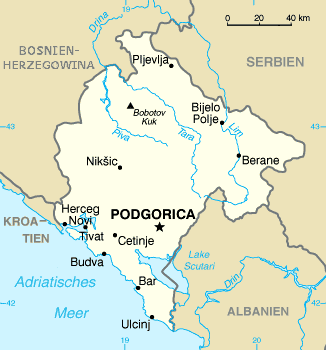
\includegraphics[width=4in]{Material/Montenegro_de}\\
 Quelle: http://upload.wikimedia.org/wikipedia/commons/0/0f/\\
Montenegro\_de.png (Aufgerufen: 10.10.2013).
\end{figure}

Montenegro besteht im Wesentlichen aus Gebirgslandschaft, hat aber auch Zugang zum Mittelmeer. Die Küstenregion ist sehr touristisch geprägt. Direkte Nachbarländer sind Albanien, Kosovo, Serbien und Bosnien-Herzegowina.


\subsubsection{Basismerkmale des Regierungssystems }

Am 19. Oktober 2007 trat eine Verfassung im selbstständigen Staat Montenegro in Kraft.\par
In der parlamentarischen Demokratie ist der Präsident das Staatsoberhaupt; er wird in direkter und geheimer Wahl für fünf Jahre gewählt. Er schlägt den Premierminister vor, der anschließend von dem 81 Abgeordnete umfassenden Parlament gewählt wird. Parlamentswahlen finden alle vier Jahre statt (\cite{osceodihr09}: 4).\par
Mit einer Fläche von 13.812 km$^2$ und ca. 600.000 Einwohnern ist Montenegro eines der kleinsten Länder Europas. Als Währung führte Montenegro unilateral zunächst die D-Mark und dann den Euro ein.\par
Außerhalb von Serbien lebt nach Bosnien-Herzegowina die prozentual größte Anzahl von Serben (30\%) in Montenegro. Dies hat in den letzten Jahren immer wieder zu politischen Auseinandersetzungen geführt. So. z.B. anlässlich der Unabhängigkeitserklärung Kosovos, die seitens der serbischen Bevölkerung in Montenegro abgelehnt, aber von den ca. 10\% montenegrinischen Albanern befürwortet wird (vgl. \cite{stanislaw}: 53).\par
In der folgenden Tabelle sind die wichtigsten Wirtschaftsdaten für Montenegro von 2007 bis 2010 überblicksartig dargestellt:

\begin{table}[H]
\setlength\belowcaptionskip{10pt}
\caption{Wirtschaftsdaten Montenegro 2007-2010}
\footnotesize
\begin{tabular}{|R{46mm}|R{25mm}|R{15mm}|R{15mm}|R{15mm}|R{15mm}|}\hline
&&2007&2008&2009&2010\\\hline
Bruttoinlandsprodukt (BIP)&
Millionen Dollar&3.668,9&4.519,7&4.141,4&4.111,1\\\hline
BIP Wachstum&\%&10,7&6,9&-5,7&2,5\\\hline
Inflation &\%&4,3&8,8&3,5&0,7\\\hline
Ausländische Direktinvestitionen &\% des BIP&25,5&21,2&36,9&18,5\\\hline
Verschuldung öffentliche Hand&\% des BIP&27,5&31,9&40,7&44,1\\\hline
\multicolumn{6}{c}{}\\
\multicolumn{6}{c}{\normalsize Quelle: \cite{bert12a}: 17 (eigene Übersetzung aus dem Englischen).}
\end{tabular}

\end{table}
 Aus dieser Tabelle ist ersichtlich, dass Montenegro ganz erheblich von der Finanzkrise betroffen war, mit stark gestiegener Verschuldung der öffentlichen Hand und rapidem Rückgang des Bruttoinlandsproduktes.

\subsubsection{Staatsaufbau und nationales Verwaltungsprofil}

Die montenegrinische Regierung hat mit Unterstützung der EU verschiedene institutionelle Reformen auf den Weg gebracht. Diese bezogen sich auf die Erbringung von öffentlichen Aufgaben, Modernisierung der Energieversorgung und den Bereich Umweltschutz. Im Fokus war auch die Reform der zentralen und lokalen Verwaltung. Korruption und politische Einflussnahme auf Medien und Justiz wurden allerdings noch im Jahr 2008 vom Europarat kritisiert, der mahnte, dass mehr für die Unabhängigkeit von Gerichten, der Anti-Korruptionseinheit und der staatlichen Medien getan werden müsse (vgl. \cite{stanislaw}: 53). Montenegro war bis zu Beginn der Wirtschaftskrise 2008 von einem beispiellosen ökonomischen Boom erfasst. Dies war zum einen der Privatisierung von Großindustrien, vor allem der Aluminiumfabrik nahe Podgorica geschuldet und zum anderen dem Aufkauf touristisch interessanter Küstengebiete, vor allem durch russische Oligarchen. Angesichts der wenig entwickelten Instrumentarien zur Finanzkontrolle in Montenegro wird vermutet, dass Geldwäsche in diesem Zusammenhang eine Rolle gespielt haben könnte (vgl. Stanislawski 2008: 55).\par
Eine Strategie zur Verwaltungsmodernisierung in Montenegro für die Jahre 2002-2009 wurde im Rahmen des mit CARDS-Mitteln finanzierten Programms „Public Administration Reform in Montenegro“ (PARIM) der European Agency for Reconstruction (EAR) vom montenegrinischen Justizministerium entwickelt. Das erklärte Ziel dieser Strategie war die stärkere Angleichung an europäische Standards und Ausdruck des Wunsches, die EU-Integration schneller voranzutreiben, was wiederum, so die Einschätzung eines Balkan-Experten, der wesentliche Treiber für die Reformbemühungen war (vgl. \cite{dzamuk}: 15).\par

Es können drei Phasen der geplanten Umsetzung der PARIM-Strategie ausgemacht werden:
\begin{enumerate}[label=Phase {\Roman*}:,align=left,  leftmargin=*] \itemsep1pt \parskip0pt \parsep0pt
\item (2002-2004) Vorbereitung
\item (2004-2007) Entwicklung
\item  (2007-2009) Vollendung
\end{enumerate}

Mit diesen drei Phasen sollten acht Punkte umgesetzt werden, um eine effektive öffentliche Verwaltung zu erreichen:
\begin{enumerate}[label= {\arabic*}),leftmargin=*]\itemsep1pt \parskip0pt \parsep0pt
\item Dezentralisierung des administrativen Systems durch Delegation der Kompetenzen auf die unteren Ebenen. Damit sollte die Flexibilität der öffentlichen Verwaltung erhöht werden und ihr mehr Handlungsspielraum zukommen.
\item Einführung einer Qualitätskontrolle bei der Vergabe von Aufträgen und Ausführung der administrativen Aufgaben.
\item Einführung kompetitiver Strukturen, die Bürgern und Unternehmen ermöglichen, ihre bevorzugten Anbieter oder Verwaltungsangebote zu wählen.
\item Kundenorientierung bei der Erfüllung öffentlicher Aufgaben.
\item Etablierung eines Personalmanagement Systems für die öffentlichen Bediensteten.
\item Modernisierung durch Informationstechnologie.
\item Entwicklung eines rechtlichen Systems, das die wichtigsten Aufgaben standardisierte und überregulierte Verwaltungsstrukturen deregulierte.
\item Verbesserung der Steuerungs- und Monitoringprozesse. (vgl. \cite{govmont03}: 19)
\end{enumerate}

Im Jahr 2003 sind etliche für die öffentliche Verwaltung relevante Gesetze verabschiedet worden: das Gesetz über staatliche Verwaltung, das die Organisation, Arbeitsweise und Funktion der staatlichen Administration beschreibt und das Gesetz zu Streitfällen, die die öffentliche Verwaltung betreffen. Das Gesetz über die staatliche Verwaltung etablierte das Prinzip, dass die Aufgaben der staatlichen Verwaltung von civil servants ausgeführt werden müssen. Aufgaben staatlicher Verwaltung werden von der Regierung, Ministerien und anderen administrativen Organen oder „agencies“ ausgeübt.

Mit dem Ziel einer modernen Verwaltung näher zu kommen wurde 2004 das Gesetz zu civil servants und Staatsbediensteten und 2005 ein entsprechendes Besoldungsgesetz verabschiedet. Eine „Human Resources Management Agency“ (HRMA) wurde gegründet, zuständig für Personalauswahl und Weiterbildung der civil servants. Weiterhin wurde 2003 ein Ombudsman’s Office eingeführt als Beschwerdeinstanz für Bürger, die mit der Verwaltung unzufrieden sind (vgl. \cite{freund07}: 2) Im Jahr 2004 wurde ein nationaler Rechnungshof eingerichtet, der laut Verfassung von 2007 eine unabhängige Institution ist, die dem Parlament berichtet (vgl. \cite{oecd08b}: 2).\par
Die Verfassung von 2007 legt in Artikel 16 die Einrichtung und die Kompetenzen der Behörden fest, Art. 20 definiert ein individuelles und kollektives Recht auf Anfechtung bei Verletzung von Rechten durch Behörden (\cite{oecd08b}: 2). Das Verwaltungsgericht erhält regelmäßig gute Noten von SIGMA: „Based on its excellent performance, the Administrative Court has become a role model throughout the public sector of Montenegro, and probably in the whole region. Its remarkable success is nevertheless endangered by the fact that its rulings against public authorities frequently cannot be effectively enforced” (\cite{oecd11a}: o.S.). Die Tradition der Verwaltungsgerichtsbarkeit in Montenegro ist positiv hervorzuheben, wobei es bei der Umsetzung der Rechtsprechung Probleme gibt. \par
Die Verantwortung für die Reform der öffentlichen Verwaltung liegt in Montenegro beim Ministerium für Inneres in der Abteilung für öffentliche Verwaltung, die unterbesetzt ist für den Umfang ihrer Aufgaben (vgl. \cite{oecd11a}: o.S.).\par
Eine neue Strategie zur Verwaltungsreform wurde im Jahr 2011 verabschiedet unter der Bezeichnung „Public Administration Reform Strategy 2011-2016“ (AURUM). Die Strategie zielt ab auf eine effiziente, professionelle, leicht erreichbare und service-orientierte öffentliche Verwaltung, die den Bürgern sowie sozialen und ökonomischen Akteuren dient. Als gesonderte Ziele wurden festgelegt:
\begin{itemize} \itemsep1pt \parskip0pt \parsep0pt
\item Stärkung des Rechtsstaates und der Verantwortlichkeit der öffentlichen Verwaltung;
Institutionelle Stabilität, Funktionalität und Flexibilität des Systems der öffentlichen Verwaltung; 
\item Bessere Bedingungen für Wirtschaftsakteure durch Verbesserung der öffentlichen Leistungserbringung und Verringerung der administrativen Belastungen; 
\item Transparentes und ethisches Handeln in der öffentlichen Verwaltung; 
\item Weitere Eingliederung Montenegros in den Europäischen Verwaltungsraum (vgl. \cite{govmont11}: o.S.).
\end{itemize}

Noch bestehende Probleme, die einer vollständigen Umsetzung der vorherigen Strategie (PARIM) zur Verwaltungsmodernisierung im Wege standen, werden ebenfalls benannt:
\begin{itemize} \itemsep1pt \parskip0pt \parsep0pt
\item Widerstände in der Verwaltung zu Beginn der Reformen;
\item Die globale Krise, die zu einer Destabilisierung der öffentlichen Finanzen und zu Haushaltsdefiziten führt;
\item Fehlen von angemessenen Mechanismen zur Verbesserung des finanziellen Status von civil servants;
\item Zu wenige junge, kreative Bewerber mit entsprechender professioneller Qualifikation;
\item Die Wahrnehmung eines hohen Grades an Bestechlichkeit in bestimmten Bereichen und Positionen;
\item Ungenügende Werbung für die Reformbemühungen und ihre Notwendigkeit;
\item Fehlen einer kompetenten Institution, die den Reformprozess mit Blick auf Professionalität und Methodologie begleitet und logistische Unterstützung zur Verfügung stellt (vgl. \cite{govmont11}: o.S.).
\end{itemize}
Die neue Strategie zur Verwaltungsreform wird von SIGMA im Kontext der bisherigen Aktivitäten Montenegros zur Verwaltungsreform kritisch beurteilt, vor allem in Hinblick auf den politischen Willen zur tatsächlichen Umsetzung: „The development of this strategy was largely driven by the perception that it was requested by donors and primarily by the EU integration process. […] The drafting of AURUM was thus heavily dependent on input from outside sources and had limited inter-ministerial co-ordination. This generates doubts on its ownership by the Government of Montenegro, concerns on the will and capacity to implement it and - finally - on its sustainability” ( \cite{oecd11a}: o.S.).
\par
Die EU beurteilt die neue AURUM-Strategie in ihrem Progress Report 2011 verhalten positiv: „The strategy includes introducing European standards covering recruitment and promotion and measures to increase the efficiency of the State administration. It also envisages an overall reduction of employment in the public sector; yet, it does not specify how this would be achieved without affecting the performance and efficiency of services. Some measures have already been taken to introduce economies of scale and integrate bodies whose activities have been disparate and uncoordinated (e.g. the various State inspection services)” (\cite{eurcom11c}: 8).\par
Die Einrichtung von neuen Institutionen in der staatlichen Administration, die sogenannte „agencification”, ist kein spezifisch montenegrinisches Phänomen. Doch für ein so kleines Land ist dieser Trend besonders problematisch, wie auch SIGMA in einem Assessment feststellt und vor weitreichenden Auswirkungen warnt: “Sometimes newly created bodies remain completely understaffed; they might exist on paper but in reality are nearly empty shells. Sometimes new mechanisms have been established in parallel to already existing institutions (departments in ministries, administrative bodies). Further ‘agencification’ is weakening the rule of law in Montenegro” ( \cite{oecd11a}: o.S.).

\subsubsection{Subnational-dezentrale Verwaltungsebene}

Die lokale Verwaltung in Montenegro basiert im Wesentlichen auf dem „Gesetz zur Lokalen Verwaltung” von 1991, das die Kommune (municipality) als Träger der lokalen Verwaltung festlegt. Auch die Verfassung von 2007 definiert die territoriale Organisation des Staates auf der Grundlage der Kommunen. In Montenegro gibt es 21 Kommunen, wobei Podgorica den Status der administrativen Hauptstadt hat und Cetinje den Status der historischen Hauptstadt. Alle Kommunen sind nach den gleichen Prinzipien organisiert, mit einem Rat und einem Bürgermeister, und haben die gleichen Kompetenzen hinsichtlich der Erbringung der lokalen Dienstleistungen. Die Kommunen werden vom Staat kontrolliert, mit der Möglichkeit den Rat und den Bürgermeister abzusetzen, wenn sie ihre Aufgaben nicht erfüllen (vgl. \cite{oecd08b}: 8). Die Kommunen haben jeweils einen für vier Jahre direkt gewählten Rat. Der Bürgermeister wird vom Gemeinderat aus seiner Mitte gewählt.\par
Die Kommune hat gesetzlich definierte Funktionen, und solche, die von der Republik zugewiesen werden können. Spezifische Aufgabenbereiche der Kommunen sind:
\begin{itemize} \itemsep1pt \parskip0pt \parsep0pt
\item Erstellung von Bebauungsplänen;
\item Bereitstellung öffentlicher Dienstleistungen;
\item Management der lokalen Wasserversorgung;
\item Zuteilung von Bauland und Erteilung von Nutzungsrechten für Büroraum;
\item Baugenehmigungen und technische Inspektionen;
\item Bau und Unterhalt von lokalen Straßen und öffentlichen Gebäuden;
\item Budgeterstellung;
\item Organisation öffentlicher PNV und Parkplätze\footnote{http://ec.europa.eu/enlargement/archives/ear/montenegro/montenegro.htm.}. 
\end{itemize}
Der wirtschaftliche Niedergang Montenegros in den 1990er Jahren als Teil des verbliebenen Rumpf-Jugoslawien betraf vor allem die Infrastruktur mit ausbleibenden Investitionen für Straßenbau, Energie-, Wasser- und Abwasserversorgung sowie Telekommunikation. Im Jahr 2000 betrug das kommunale Budget für das Jahr ca.  \euro{}  1,3 Millionen pro Kommune, wobei die Hauptstadt Podgorica  \euro{}  7,0 Millionen zur Verfügung hatte und die am wenigsten entwickelte Kommune  \euro{} 200.000.\footnote{http://ec.europa.eu/enlargement/archives/ear/montenegro/montenegro.htm.}\par
Während in den Republiken der SFR Jugoslawien eine Tradition der Selbstverwaltung bestand, führte die starke Kontrolle durch die Kommunistische Partei dazu, dass die Kommunen administrativ nicht in der Lage waren, eigenständig Aufgaben zu planen und auszuführen. Die schnelle Dezentralisierung seit der Demokratisierung, oft durch internationalen Einfluss in den neu entstandenen Ländern durchgesetzt, wurde nicht durch entsprechende fiskale Dezentralisierung begleitet, und die Kontroll- und Prüfmechanismen auf lokaler Ebene waren nicht ausgebildet. „Over-hasty and ambitious decentralisation has increased the risk of corruption and misuse of public monies across the region, without really increasing local autonomy and accountability” (\cite{oecd04}: 10).\par
Institutionell wird die Umsetzung der Reform der lokalen Verwaltung von einer Abteilung im Innenministerium begleitet und überwacht. Das Committee for Coordination of Local Self-Government Reform (CCLSGR) wurde 2007 etabliert und sorgt für Dialog, Kooperation und Koordination zwischen zentraler und lokaler Verwaltung. Darin vertreten sind das Finanzministerium, das Innenministerium, die Vereinigung der Kommunen, die seit 1972 besteht, sowie fünf Kommunen (rotierend). Drei Komitees arbeiten zu den Themen Internationale Kooperation, Dezentralisierung der Finanzen und Administrative Dezentralisierung. \par
Montenegro hat die Europäische Charta der Kommunalen Selbstverwaltung im Jahr 2008 unterzeichnet und die Regierung führte im Sommer 2009 eine 60-tägige öffentliche Debatte durch zum Gesetzesentwurf „on Territorial Organisation“. Das Gesetz trat 2011 in Kraft.\footnote{http://assembly.coe.int/ASP/Doc/XrefViewPDF.asp?FileID=18947 (Aufgerufen: 1.9.2012).} 


\subsubsection{Öffentlicher Dienst }
1999 wurden offizielle Zahlen für den föderalen civil service des damaligen Rumpf-Jugoslawien mit 12.000 Beschäftigten angegeben. Daneben waren 80.000 Beschäftigte im civil service Serbiens tätig. Zahlen für Montenegro wurden nicht veröffentlicht, beliefen sich aber geschätzt auf 20.000 civil servants in Montenegro (vgl. \cite{sevic}: 57).\par
Das Gesetz „on Civil Service and State Employees“ von 2004 definiert civil servants und state employees als Beschäftigte, die administrativ für die Umsetzung der Kompetenzen einer staatlichen Institution tätig werden. Somit sind beide im Prinzip von der Tätigkeit her gleichgestellt, mit der Ausnahme, dass state employees (die z.B. im staatlichen Pensionsfonds oder dem staatlichen Gesundheitssystem arbeiten) fiskalische und technische Funktionen haben, die für civil servants nicht erwähnt sind. Der civil service ist als System nach der Position (position based) etabliert und nicht am Leistungsgedanken (merit based) orientiert. \par
Auch die neue Verfassung von 2007 differenziert nicht zwischen Beamten und anderen öffentlichen Angestellten (vgl. \cite{oecd08c}: 1). Im Gegensatz zu der Praxis in den meisten EU-Ländern enthält die Verfassung keine Referenz zu Unparteilichkeit der staatlichen Bediensteten, der Einstellung aufgrund von Fähigkeiten sowie einem transparenten und kompetitiven Einstellungssystem. Andererseits gibt es in der Verfassung einige wichtige Vorschriften, die im Zusammenhang mit der weiteren Reform der öffentlichen Verwaltung bedeutsam sein könnten. So ist beispielsweise jegliche politische Organisation in der staatlichen Verwaltung verboten. Allerdings wurde im Gegensatz zu der vorherigen Verfassung von 1992 nicht aufgenommen, dass öffentliche Bedienstete ihre Aufgaben verantwortlich und ehrlich erfüllen müssen und für ihr Handeln zur Rechenschaft gezogen werden können (vgl. \cite{dzamuk}: 19). \par
Für die Umsetzung der Personalangelegenheiten des civil service und der state employees wurde die Human Resource Management Agency (HRMA) als staatliche Institution im Jahr 2004 gegründet. Die HRMA ist zuständig ist für die Veröffentlichung von Stellenanzeigen, die Selektion von Personal nach etablierten Regeln, für Stellenbeschreibungen, ein Register von civil servants und deren Weiterbildung (\cite{vukovic}: o.S.)\par	
Die Gesetzgebung zum civil service wurde von SIGMA und der EU kontinuierlich kritisiert. Exemplarisch sei dazu folgende Einschätzung wiedergegeben: „The current Law on Civil Servants and State Employees does not provide a clear legal definition of the scope of the civil service, which would help to establish rights and obligations as well as the accountability and liability of all civil servants at both national and municipal levels. Furthermore, it does not fully reflect the merit principle in recruitment and promotion. Finally, a new civil service law needs to include a special regulation for civil servants on conflict of interest, incompatibilities, gift policies, and whistle blowing. The current Law on Conflict of Interest does not provide a satisfactory solution, mainly because it encompasses both politicians and civil servants, which are two groups representing different realities and having different regulatory requirements” (\cite{oecd10a}: 3).\par
Ein neues meritokratisches Gesetz zu civil servants und state employees wurde Mitte 2011 verabschiedet und soll zusammen mit einem transparenteren Besoldungssystem 2013 in Kraft treten. Auch die HRMA wurde gestärkt und ihr wurde eine aktive Rolle in der Entwicklung von Personalplanungskonzepten zugewiesen. 2011 hatte die HRMA 36 Beschäftigte, soll aber zur effektiven Umsetzung der neuen Gesetzgebung zum civil service und state employees auf 52 Beschäftigte aufgestockt werden.\par
Zusammengefasst zeigt sich, dass in Montenegro die öffentliche Verwaltung in der Demokratie zu einem erheblichen Teil von der Praxis in Jugoslawien geprägt war und ist. In Montenegro wurde der Umbau der öffentlichen Verwaltung seit dem demokratischen Wechsel Anfang der 1900er Jahre ab 2002 von einer umfassenden Strategie (PARIM) begleitet, die unter Federführung der EU entwickelt wurde. Wesentliche Modernisierungsbemühungen haben stattgefunden, allerdings mit mäßigem Erfolg. Eine neue Strategie zur Verwaltungsmodernisierung im Zusammenhang mit der EU-Annäherung trat 2011 in Kraft. \par
Die bestehenden Probleme der Modernisierung der öffentlichen Verwaltung in Montenegro sind zu einem erheblichen Teil mit der Entwicklung in Jugoslawien zu erklären. In der Demokratie war das bisherige jugoslawische Konzept der public sector employees weiterhin bestimmend. Historisch gesehen (vor der SFR Jugoslawien) bestand jedoch in Montenegro eine klare Trennung von Beamten und anderen öffentlich Angestellten und eine Wiederannäherung an diese kontinentaleuropäische Tradition scheint daher möglich. \par
Das starke Weiterwirken der jugoslawischen Traditionen zeigte sich auch im von Verhältnis Zentralregierung und lokaler Ebene. Während der lokalen Ebene in der jugoslawischen Zeit einerseits große Bedeutung zukam (Stichwort: Selbstverwaltungssozialismus), war diese Ebene der Verwaltung andererseits durch den starken Einfluss der Kommunistischen Partei, die stark zentralistisch organisiert war, nicht eigenständig handlungsfähig. Dieses Erbe wurde in der demokratischen Zeit deutlich, als die lokale Ebene im Zuge der Dezentralisierung und im Rahmen der Annäherung an europäische Standards vermehrt Kompetenzen zugesprochen bekam. Die verabschiedeten Konzepte der Dezentralisierung fruchteten in der Praxis allerdings kaum, aufgrund von fehlender Erfahrung der Zusammenarbeit sowie Aufgabenteilung zwischen lokaler und zentraler Verwaltung. Weiterhin hat die fiskalische Dezentralisierung nicht in gleichen Maß stattgefunden wie die Übertragung von Aufgaben.
\par
Ein spezifisches Phänomen in Montenegro, das sich so nicht in den anderen beiden Untersuchungsländen wiederfindet, ist die Bedeutung von unregulierten Finanzflüssen auf Wirtschaft und Gesellschaft. In den 1990er Jahren während der Jugoslawienkriege entwickelte sich eine Schattenökonomie und in den 2000er Jahren bis zur Finanzkrise 2008 investierten vor allem russische Oligarchen in der montenegrinischen Küstenregion mit entsprechendem, zum Teil unregulierten Geldzufluss.
\subsection{Mazedonien} 
Mazedonien erklärte nach einem Referendum 1991 die Unabhängigkeit von Jugoslawien und eine neue Verfassung legte im gleichen Jahr die Grundlage für den Staat. Mazedonien war in Bezug auf Infrastruktur und Wirtschaftskraft der am wenigsten entwickelte Staat, der aus der SFR Jugoslawien hervorging. Obwohl Mazedonien nicht direkt an den Balkankriegen (1991 bis 1995) beteiligt war, hatten diese doch einen enormen ökonomischen Effekt auf das Land. Eine Wirtschaftskrise in Mazedonien von 1991-1993 resultierte zum großen Teil aus den Folgen der Sanktionen der Vereinten Nationen gegenüber Serbien, das Mazedoniens Haupthandelspartner war. Ein ökonomischer Stabilisierungsplan des IMF und der Weltbank stellten die makroökonomische Stabilität Mitte der 1990er Jahre wieder her (vgl. \cite{bech09}: lxix). 
\begin{figure}[H]
\setlength\belowcaptionskip{10pt}
 \caption{Landkarte Mazedonien}
  \centering
  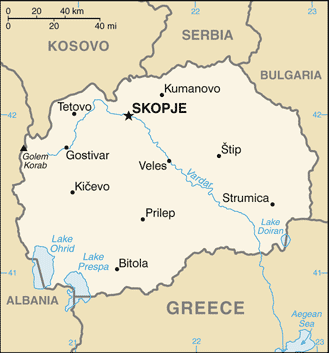
\includegraphics[width=4in]{Material/Macedonia-CIA_WFB_Map}\\
 Quelle: http://commons.wikimedia.org/wiki/\\
File:Macedonia-CIA\_WFB\_Map.png (Aufgerufen: 10.10.2013).
\end{figure}

Aus der Karte ist die geografische Lage Mazedoniens ersichtlich als ein Land ohne Meereszugang. Die Hauptstadt ist Skopje. Mazedonien hat fünf direkte Nachbarstaaten: Serbien, Bulgarien, Griechenland, Albanien und Kosovo. Das Land ist 25,713 km$^2$ groß und hat etwas über 2 Millionen Einwohner (vgl. \cite{ramet}: 785). 

\subsubsection{Basismerkmale des Regierungssystems}

Mazedonien ist eine parlamentarische Demokratie. Staatsoberhaupt ist der Staatspräsident, der vom Volk für fünf Jahre gewählt wird, allerdings wesentlich weniger Machtbefugnisse hat als der Premierminister. Der Präsident beruft den Premierminister aus der Partei oder Koalition, die die Mehrheit im Parlament stellt. Das Parlament hat 123 Abgeordnete, die mittels Verhältniswahl gewählt werden (vgl. \cite{osceodihr11}: 2). Unter den 18 Ministerien ist eines für die Umsetzung des Rahmenabkommens von Ohrid zuständig (vgl. \cite{markic}: 3).\par
Mehrere 100.000 Mazedonier leben im Ausland. Neben Mazedoniern, die ca. 65\% der Bevölkerung stellen, leben ca. 25\% Albaner in Mazedonien, was immer wieder zu Konflikten zwischen der Mehrheits- und der Minderheitsgruppe führt.\footnote{Andere Minderheiten umfassen Türken (3,85 \%), Roma (2,66 \%), Serben (1,78 \%), Bosniaken (0,84 \%), Aromunen/Meglenorumänen (0,48 \%) und andere (1,04 \%).} Gewalttätige Ausschreitungen im Jahr 2001 durch albanische Guerilla-Gruppen im Norden Mazedoniens lösten eine Krise aus, die nur mit internationaler Vermittlung entschärft werden konnte. Es kam zur Unterzeichnung des Ohrid-Rahmenabkommens im August 2001 in der mazedonischen Stadt am Ohrid-See.\footnote{Das Ohrid-Abkommen hat zum Inhalt: 1. Friedenssicherung (Artikel 1 und 2), 2. Dezentralisierung und Symbolgebrauch; 3. Minderheitenregelungen; sowie 4. Bildung und Sprachgebrauch.} Das Abkommen führte zu größeren politischen Beteiligungsrechten der Albaner mit einer doppelten Mehrheit für Parlamentsentscheidungen zu bestimmten Themen, die von besonderem Interesse für Minderheiten sind. In diesen Fällen ist eine Mehrheit aller Abgeordneten und eine Mehrheit der nicht-mazedonischen Abgeordneten notwendig (Badinter-Prinzip)\footnote{Benannt nach dem früheren französischen Justizminister Robert Badinter, der an den Ohrid-Verhandlungen beteiligt war.} (vgl. \cite{szpala}: 60).\par
In der folgenden Tabelle sind die wichtigsten Wirtschaftsdaten für Mazedonien von 2007 bis 2010 überblicksartig dargestellt:
\begin{table}[H]
\caption{Wirtschaftsdaten Mazedonien 2007-2010}
\footnotesize
\begin{tabular}{|R{46mm}|R{25mm}|R{15mm}|R{15mm}|R{15mm}|R{15mm}|}\hline
&&2007&2008&2009&2010\\\hline
Bruttoinlandsprodukt (BIP)&
Millionen Dollar&8159,8&9834&9313,6&9189,5\\\hline
BIP Wachstum&\%&6,1&5&-0,9&1,8\\\hline
Inflation &\%&3,6&7,2&-0,3&2,1\\\hline
Ausländische Direktinvestitionen &\% des BIP&8,6&6&2,1&3,2\\\hline
Verschuldung öffentliche Hand&\% des BIP&24&20,6&23,9&24,8\\\hline
\multicolumn{6}{c}{}\\
\multicolumn{6}{c}{\normalsize Quelle: \cite{bert12b}: 18 (eigene Übersetzung aus dem Englischen).}
\end{tabular}\\
\end{table}

In der Tabelle ist erkennbar, dass Mazedonien trotz Finanzkrise, die das Land in der Wirtschaftsentwicklung verlangsamt hat, dennoch die Staatsverschuldung stabil halten konnte.
\subsubsection{Staatsaufbau und nationales Verwaltungsprofil}
Folgende Funktionen sind in der Verfassung festgelegt: der Staatliche Justizrat mit sieben vom Parlament ernannten Mitgliedern, der für die Verwaltung der Justiz zuständig ist und dem Parlament die Richter vorschlägt; das Büro der Ombudsperson, die vom Parlament für acht Jahre (erneuerbar) ernannt wird; der Rechnungshof, der dem Parlament berichtet; die Agentur für Civil Servants (CSA) mit einem Direktor, der/die für sechs Jahre ernannt wird. \par

Der bisherige Reformprozess der öffentlichen Verwaltung in Mazedonien kann in zwei Phasen eingeteilt werden: 
\begin{enumerate}[label= {\alph*}), leftmargin=*] \itemsep1pt \parskip0pt \parsep0pt
\item Bis zum Jahr 1998 wurden bestimmte Maßnahmen eingeführt, die das System im Rahmen eines systematischen und kohärenten Ansatzes verbessern und effizienter machen sollten. Zu diesen Entwicklungen gehörten u.a. die Einführung eines Rechnungshofes (State Audit), die Einrichtung des Büros der Ombudsperson, Regeln für öffentliche Anschaffungen und ein Budgetgesetz.
\item Nach der Entwicklung der ersten Strategie zur Reform der Öffentlichen Verwaltung im Jahr 1999. 
\end{enumerate}

Die Veränderung der öffentlichen Verwaltung von einem Ausführungs- und Kontrollorgan des Staates hin zu eher regelnder Funktion wurde vorangetrieben durch die Erfordernisse der Marktwirtschaft und die Einleitung einer Annäherung an die EU. Eine „Strategie der Reform der Öffentlichen Verwaltung“ wurde im Mai 1999 angenommen und definierte Prinzipien für die öffentliche Verwaltung, Reformziele und Sektorprioritäten. Als Prinzipien für die öffentliche Verwaltung wurden festgelegt: Rechtsstaatlichkeit, Transparenz, Stabilität, Verantwortlichkeit, Verlässlichkeit, Gleichbehandlung, Effizienz und Ethik.
Als wesentliche Bereiche für die Reform wurden definiert:
\begin{itemize} \itemsep1pt \parskip0pt \parsep0pt
\item „State administration system;
\item Public administration system;
\item Local self-government system;
\item Redefining the role of the State;
\item Exercise and protection of citizen’s rights;
\item Public finance restructuring; and
\item IT system development” (\cite{analyt07}: 7).
\end{itemize}
Ende der 1990er Jahre dominierten zunächst andere Themen Politik und Verwaltung in Mazedonien. Die Kosovo-Krise 1999 brachte Flüchtlingsströme, die versorgt werden mussten, über die Grenze. Im Jahr 2001 brachen dann gewalttätige ethnische Konflikte im Norden Mazedoniens aus, zu deren Beilegung internationale Vermittlung notwendig wurde. \par
Das Ohrid-Rahmenabkommen von 2001 hatte umfassende Auswirkungen auf die weitere Reform des Staates und der öffentlichen Verwaltung. Darin enthalten waren Lösungen für den Zugang zu öffentlichen Ämtern, den Sprachgebrauch, den Status der albanischen Minderheit und die Dezentralisierung.\par
Zur Überwachung der Umsetzung der Reform der öffentlichen Verwaltung wurde eine Kommission für Verwaltungsreform mit mehreren Arbeitsgruppen im Justizministerium eingesetzt. Diese Kommission wurde im Jahr 2002 durch eine Abteilung für Verwaltungsreform im Sekretariat der Regierung ersetzt (vgl. \cite{analyt07}: 7). Eine erneute Änderung der Zuständigkeiten führte 2011 dazu, dass die Koordination für die Verwaltungsreform nun im Ministerium für Verwaltung und Information angesiedelt ist.\par
Projekte zur Verwaltungsreform und insbesondere zur Umsetzung des Ohrid-Abkommens wurden von der EU sowie von einer Vielzahl anderer Geber und Akteure vorangetrieben. Ebenso ist eine erneute strategische Standortbestimmung zur Reform der öffentlichen Verwaltung für die Jahre 2010-2015 mit finanzieller Unterstützung der EU verabschiedet worden. Wesentliche Ziele der neuen Strategie sind Verbesserungen in den Bereichen öffentliche Finanzen, Human Resources Management, e-government und Korruptionsvermeidung (vgl. \cite{dimeski}: 7). \par
Die Qualität der neuen Strategie für Verwaltungsreform wird von einheimischen Experten gewürdigt. Jedoch wird auf die Probleme mit der Umsetzung der bisherigen Strategie verwiesen und mit dem Bekenntnis der verschiedenen Regierungen zu Verwaltungsmodernisierung streng ins Gericht gegangen. Es wird konstatiert, dass es an Umsetzungswillen und effektivem Management des Prozesses der Verwaltungsmodernisierung mangelte (vgl. \cite{dimeski}: 11).

\subsubsection{Subnational-dezentrale Verwaltungsebene}
Mazedonien hat eine bipolare Verwaltungsstruktur mit Kommunen und Zentralregierung, ohne intermediäre Ebene. Während die Dezentralisierung schon in der Strategie für die Verwaltungsreform von 1999 als Ziel formuliert war, führte das Ohrid-Rahmenabkommen zu einem Schub der Dezentralisierungsbemühungen mit der Einbeziehung von Minderheiten auf der lokalen Ebene. Das Ministerium für Lokale Selbstverwaltung war zuständig für die Koordination der Dezentralisierung, inklusive der finanziellen Aspekte. Auch der Zusammenschluss der Kommunen „Association of the Units of Local Self-Government“ (ZELS) ist ein wichtiger Akteur und Ansprechpartner für die Kommunen im Prozess der Dezentralisierung (vgl. \cite{analyt07}: 10).\par
Wie in Artikel 3 des Ohrid-Rahmenabkommens vorgesehen, verabschiedete das Parlament ein neues Gesetz zur lokalen Selbstverwaltung (2002). In Artikel 22 dieses Gesetzes sind die Bereiche aufgeführt, die an die Ebene der Gemeinden abgegeben werden sollen: (i) Stadtplanung und ländliche Entwicklung; (ii) Umweltschutz; (iii) lokale Wirtschaftsentwicklung; (iv) kommunale Dienstleistungen (unter anderem: Wasserversorgung, Abwasserbehandlung, Müllbeseitigung und -behandlung, Zurverfügungstellung von Wärmeenergie und Straßenbau; (v) Kultur; (vi) Sport- und Freizeiteinrichtungen; (vii) Sozialwesen; (viii) Bildung; (ix) Gesundheit; (x) Zivilschutz; (xii) Feuerwehr; (xii) Überwachung von kommunalen Aufgaben und (xiii) andere gesetzlich definierte Aktivitäten.\par
In Ergänzung zu dem Gesetz entwickelte die Regierung einen Ausführungsplan für die Dezentralisierung für 2003-2004. Für die Umsetzung war das Ministerium für Lokale Verwaltung zuständig. Im Jahr 2004 trat dann das neue Gesetz zur Territorialverwaltung in Kraft, das Mazedonien in acht Regionen mit 84 Gemeinden einteilte. Die bisherigen 123 Gemeinden wurden teilweise zusammengefasst, nur im Verwaltungsraum der Hauptstadt Skopje wurden die bisher acht Gemeinden auf zehn erhöht. Die Umsetzung der Dezentralisierung begann offiziell im Juli 2005 mit der vorgesehenen territorialen Reorganisation. \par
Wie in anderen vormals zentralistisch organisierten Ländern, verlief der Prozess der Dezentralisierung in Mazedonien nicht reibungslos. Der Transfer von Kompetenzen von der zentralen Verwaltung auf die Kommunen begann für verschiedene Bereiche im Jahr 2005. In einem ersten Schritt wurde die Steuererhebung von Einkommenssteuer, Mehrwertsteuer und Grundsteuer an die Kommunen abgegeben. In einem zweiten Schritt, der auf die Zeit ab 2008 verschoben wurde, sollten Zuweisungen z.B. für Bildung an die lokale Verwaltungsebene fließen. Problematisch für die lokale Ebene sind auch die geringen eigenen Steuereinnahmen (vgl. \cite{repofmac12}: 55). Die Europäische Kommission kommentierte 2006: „In many cases, municipalities are far from ready to take on their newly devolved responsibilities and central ministries remain unsure of their role in the process. Therefore, operational and financial support to line ministries and municipalities will remain crucial. Weaker municipalities will need greater direction and support with an equalisation procedure to correct any imbalance. Bringing the process of decentralisation to a good end is without doubt one of the main challenges the country faces” (\cite{ear}: o.S.). Hingewiesen wurde von der EU auch auf die nicht entwickelten Systeme der Finanzkontrolle, die nötig wären, um die Veruntreuung öffentlicher Gelder auf kommunaler Ebene zu verhindern. Unter CARDS 2004 waren einige Überprüfungen der Finanzen auf lokaler Ebene als Pilot-Projekte geplant, doch fehlende politische Unterstützung durch die Gemeinden, die keine lokalen Prüfer ernannten, und Widerstände der Mitarbeiter der lokalen Verwaltung verhinderten eine erfolgreiche Umsetzung unter „local ownership“ (vgl. \cite{eurcom06a}: 3).

\subsubsection{Öffentlicher Dienst}
Schon 1990 im Systemübergang wurde das Gesetz für die Verwaltungsorgane erlassen, das den Status der Beschäftigten in der staatlichen Verwaltung definierte. In der sozialistischen Geschichte ist der besondere Status der öffentlich Bediensteten zugunsten einer Gleichstellung mit anderen Arbeitnehmern befördert worden, was unter anderem zu einer Entprofessionalisierung führte. Dem versuchte im Jahr 2000 das Gesetz über civil servants entgegenzuwirken, mit dem Ziel die Bedingungen für einen professionellen, politisch neutralen, kompetenten, verantwortlichen und stabilen civil service herzustellen, der effizient im Sinne der Bürger und Wirtschaft arbeitet. Das Gesetz beschreibt den Begriff der civil servants. Diese sind bei den staatlichen Institutionen der Exekutive, Legislative oder Judikative angestellt, arbeiten als Experten und entscheiden über administrative Vorgänge, basierend auf der Verfassung und den Gesetzen. (vgl. \cite{markic}: 12). Im Gegensatz zu den meisten Ländern in West- und Osteuropa handelt es sich nicht um ein Karrieremodell, sondern ist „position based“. Das Gesetz wurde mehrmals geändert, unter anderem, um die Bestimmungen des Ohrid-Abkommens zur gleichberechtigten Teilhabe der Minderheiten umzusetzen. \par
Ebenfalls im Jahr 2000 wurde eine  „Strategy for Civil Servants Training in the Process of Macedonia's Approximation to the European Union“ angenommen. Auch die Civil Servants Agentur (CSA) wurde im Jahr 2000 als eigenständige Institution aufgebaut. Sie ist verantwortlich für die Personalentwicklung, das Vorbereiten von Sekundärgesetzgebung im Bereich civil servants, die Koordination von Schulungen, Systematisierung von Stellenbeschreibungen und Stellenanzeigen. Außerdem ist die CSA zweite Instanz in Beschwerdeverfahren von civil servants. Der Direktor der CSA muss dem Parlament jährlich einen Tätigkeitsbericht vorlegen. Weiterhin ist es Aufgabe der CSA, ein nationales Register für civil servants zu führen. Laut CSA gab es im Jahr 2011 auf nationaler Ebene 10.000 und auf lokaler Ebene 1.800 civil servants. Diese Zahl erhöht sich insgesamt auf ca. 32.000, wenn man Armee und Polizei mitrechnet (\cite{repofmac04}: 201). \par
Zurzeit arbeiten insgesamt etwa 110.000 Beschäftigte in der öffentlichen Verwaltung (ausgenommen Beschäftigte in Staatsbetrieben), davon sind ca. 42.500 in der Staatsverwaltung, ca. 33.500 in Bildung und Wissenschaft und ca. 33.000 im Gesundheitssystem tätig. Damit macht die Beschäftigung im öffentlichen Sektor rund 12\% der Erwerbsbevölkerung aus, eine Quote vergleichbar mit anderen Ländern Zentral- und Osteuropas. In Mazedonien werden ca. 6\%-7,5\% des Haushaltes für Gehälter der öffentlichen Verwaltung ausgegeben (vgl. \cite{analyt09}: 4).\par
Neben der Definition von civil servants gab es keine Definition oder Regelung für die ‘public employees’, das sind Personen, die im öffentlichen Sektor arbeiten, aber keine civil servants sind. Auf die public employees, die die Mehrheit der im öffentlichen Sektor Tätigen stellen, trifft lediglich das Arbeitsgesetz zu, was Tür und Tor öffnete für Missbrauch der Regelungen und für das Einsetzen politisch opportuner Kandidaten der jeweiligen Regierung (vgl. \cite{analyt07}: 16). Die EU beschrieb darüber hinaus immer wieder die problematische Praxis von temporären Verträgen, unter Umgehung der vorgeschriebenen Rekrutierungsverfahren. In den letzten Jahren wurden viele dieser temporären Positionen in permanente umgewandelt, was der Kritik weiter Vorschub leistete, da oft keine ausreichenden Begründungen und Qualifikationsnachweise zugrunde gelegt wurden (vgl. \cite{eurcom11b}: 10). Da die Anzahl der Beschäftigten überdies die Zahl der real existierenden Arbeitsplätze übersteigt, gelangten immer öfter Meldungen an die Öffentlichkeit über Verwaltungsangestellte, die formal eingestellt sind und regelmäßig Lohn beziehen, jedoch keine Arbeit leisten müssen (vgl. \cite{malahova}: 8).\par
Die oft kritisierten Lücken in der Gesetzgebung wurden nun teilweise geschlossen durch ein Gesetz zu „public employees“, seit April 2011 in Kraft, das sich der großen Gruppe der öffentlich Beschäftigten annimmt, die keine civil servants sind. SIGMA bleibt jedoch kritisch: “The law suffers from serious shortcomings in terms of both methodology and content. The structure is unsystematic and inconsistent. The regulatory content fails to make a clear distinction between civil servants and public employees and, more over contains numerous substantive (material) regulations that are inappropriate and will cause problems and confusion when the law has to be implemented. The provisions on recruitment procedures do not exclude arbitrariness; rules on promotion do not exist; mobility is badly regulated; and the six biannual appraisals will impose an unbearable administrative burden on managers” (\cite{oecd10c}: 5).\par
Nach Kritik an der halbherzigen Umsetzung der Vereinbarungen des Ohrid-Rahmenabkommens zum Minderheitenzugang zur öffentlichen Verwaltung wurde auch in dieser Hinsicht nachgebessert und 1.600 civil servants von Nicht-Mehrheitskommunen eingestellt. Die Europäische Kommission kommentierte dies als Erfüllung der Vorgaben in quantitativer Hinsicht, ohne Einbeziehung der Bedarfe in den entsprechenden Institutionen: „However, the trend of recruiting employees from these communities on a quantitative basis without regard to the real needs of the institution continued”, und ergänzt: „The recruitment procedure remains vulnerable to undue political influence“ (\cite{eurcom11b}: 10).\par
Zusammengefasst zeigt sich, dass Verwaltungsmodernisierung in Mazedonien in den Anfangsjahren der Demokratie zwar ab 1999 von einer Strategie geleitet war, es aber andere Themen gab, die politische Priorität hatten. Eine spezielle Gesetzgebung führte zur Einstellung von Minderheiten in der öffentlichen Verwaltung. Insgesamt zeigt sich, dass das Bekenntnis des Landes zur Reform der öffentlichen Verwaltung von nationalen und internationalen Beobachtern weitgehend als Lippenbekenntnis eingeschätzt wird.\par
Einer der mazedonischen Think Tanks stellt die Anstrengungen Mazedoniens zu der Modernisierung der öffentlichen Verwaltung in Frage und sieht die EU als wesentlichen Treiber der Verwaltungsmodernisierung. Gleichzeitig werden die etablierten Praxen, die vor allem den politischen Eliten dienen, beibehalten: „The Public Administration (PA) in Macedonia, even after its succession from Yugoslavia, has functioned according to the same old principles, which have served well the interests of the governing political parties. Efforts to reform the PA have come only due to the fact that Public Administration Reform (PAR) stands as an important precondition for Macedonia’s accession in the EU” (\cite{analyt11}:  o.S.).\par
Ob konkrete Schritte der erneuerten Strategie zur Verwaltungsreform von 2011 folgen werden, bleibt abzuwarten. Der Missbrauch von Stellenbesetzungen im öffentlichen Bereich wurde bislang als besonders problematisch erlebt. 

\subsection{Albanien}
Anders als Jugoslawien, das nach der sozialistischen Staatsgründung eine graduelle, vor allem wirtschaftliche Öffnung praktizierte, hatte das kommunistische und international vollständig isolierte System in Albanien ein wirtschaftlich vollkommen rückständiges Land hinterlassen. Albanien war nach dem Ende des kommunistischen Regimes von Hilfsleistungen und internationaler Unterstützung abhängig. Die wirtschaftlich prekäre Lage führte dazu, dass viele Albaner versuchten ihr Land zu verlassen. Betrügerische Systeme zur Geldanlage, in die mehr als die Hälfte der albanischen Bevölkerung investiert hatte, brachen 1997 zusammen und große Teile der Bevölkerung verloren alle Ersparnisse. In der Folge kam es zu bürgerkriegsähnlichen Ausschreitungen. Die Situation konnte nur mit internationaler Hilfe entschärft werden und stellte eine schwerwiegende Krise für die neue Demokratie dar (vgl. \cite{jarvis}: 11).
\begin{figure}[H]

  \caption{Landkarte Albanien}
  \centering
  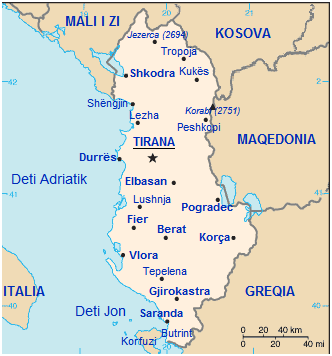
\includegraphics[width=4in]{Material/AlbanianMapShqip}\\
  Quelle: http://de.wikipedia.org/wiki/Datei:AlbanianMapShqip.png (Aufgerufen: 10.10.2013).
\end{figure}
Aus dieser Karte ist ersichtlich, dass Albanien eine lange Küste am Mittelmeer hat. Diese ist aber touristisch noch wenig erschlossen. Albanien hat 28.748 km$^2$ und ca. 3,2 Millionen Einwohner. Die Hauptstadt ist Tirana. Direkte Nachbarstaaten von Albanien sind Griechenland, Mazedonien, Kosovo und Montenegro.

\subsubsection{Basismerkmale des Regierungssystems}
Seit den ersten freien Wahlen von 1991 ist Albanien eine parlamentarische Republik mit einer zentralen Regierung und lokalen Regierungsstrukturen. Gesetzgeber ist die Versammlung der Republik Albaniens, deren 140 Abgeordnete alle vier Jahre gewählt werden. Staatsoberhaupt ist der vom Parlament auf fünf Jahre gewählte Präsident. Die dem Parlament verantwortliche Regierung wird vom Ministerpräsidenten geführt. Dieser ernennt die Minister, die vom Präsidenten bestätigt werden müssen. Die derzeit gültige Verfassung wurde am 28. November 1998 durch eine Volksabstimmung angenommen (vgl. \cite{oeza06}: 8). Kennzeichnend für die politische Kultur in Albanien ist das Fehlen einer konstruktiven Zusammenarbeit zwischen den beiden größten politischen Parteien, was vielfach zu Blockadesituationen auch im Parlament führt. Im legislativen Prozess ist für bestimmte wichtige Gesetze eine 3/5-Mehrheit der Abgeordneten nötig, die nur durch Zusammenarbeit und Kompromisse der zwei fast gleich starken Parteien zustande kommen kann. Auch auf die lokale Ebene hat die Polarisierung zwischen den beiden größten Parteien Auswirkungen, wie immer wieder an Kontroversen zwischen oppositionsgeführten Kommunen und der Zentralregierung deutlich wird. Ein Projekt allerdings wurde und wird von allen politischen Kräften in Albanien vertreten: Das Ziel der Aufnahme Albaniens in die EU.\par
In der folgenden Tabelle sind die wichtigsten Wirtschaftsdaten für Albanien von 2007 bis 2010 überblicksweise dargestellt:
\begin{table}[H]

\caption{Wirtschaftsdaten Albanien 2007-2010}
\footnotesize
\begin{tabular}{|R{46mm}|R{25mm}|R{15mm}|R{15mm}|R{15mm}|R{15mm}|}\hline
&&2007&2008&2009&2010\\\hline
Bruttoinlandsprodukt (BIP)&
Millionen Dollar&10704,7&12968,7&12044,9&11786,1\\\hline
BIP Wachstum&\%&5,9&7,7&3,3&3,5\\\hline
Inflation &\%&2,9&3,4&2,3&3,5\\\hline
Ausländische Direktinvestitionen &\% des BIP&6,2&7,4&8,0&9,4\\\hline
Verschuldung öffentliche Hand&\% des BIP&53,8&55,2&60,2&59,7\\\hline

\multicolumn{6}{c}{}\\
\multicolumn{6}{c}{\normalsize Quelle: \cite{bert12c}: 16 (eigene Übersetzung aus dem Englischen).}
\end{tabular}
\end{table}

Aus dieser Tabelle ist erkennbar, dass die Staatsverschuldung Albaniens seit 2007 bei über 50\% liegt und sich in Folge der Finanzkrise noch etwas erhöht hat, sich aber auf diesem hohen Niveau zu konsolidieren scheint. Das Bruttoinlandsprodukt, das 2008 noch 7,7\% betrug, hat sich infolge der Finanzkrise halbiert, ist aber immer noch positiv.

\subsubsection{Staatsaufbau und nationales Verwaltungsprofil}
Der Aufbau einer funktionsfähigen Verwaltung war eines der Hauptziele nach dem Systemwechsel. In den 1990er Jahren lag das Hauptaugenmerk vor allem auf der Entwicklung einer funktionsfähigen Zentralregierung nach demokratischen Prinzipien. Auch die Neuausrichtung im makroökonomischen Bereich und im Bankwesen, sowie die Privatisierung waren vorrangige Ziele dieser Zeit. Albanien erhielt Unterstützung durch das EU-Programm PHARE. Prioritäten waren die Entwicklung eines Dienstrechts für den öffentlichen Dienst und ein Management-System für öffentliche Ausgaben. Während an gesetzlichen Grundlagen für eine moderne öffentliche Verwaltung gearbeitet wurde, blieb die Umsetzung und Durchsetzung der Standards gering. Auch gab es in Albanien nach der Demokratisierung des Landes keine unabhängige Kontrolle von Regierung und Verwaltung. Die Verfassung überträgt dem Ministerrat (council of ministers) umfangreiche Kompetenzen unter anderem dann, wenn eine Funktion nicht an ein anderes Organ oder die lokale Verwaltung zugewiesen wird. Dies wird oft als verfassungsmäßige Grundlage für die Ermächtigung der Verwaltung angewandt (vgl. \cite{oecd08a}: 2). Erst 1999 wurde ein Verwaltungsverfahrensgesetz eingeführt mit neuen Kontrollmechanismen für die öffentliche Verwaltung, das zu mehr Verantwortlichkeit führen sollte, ein Anspruch, der in der Praxis allerdings oft keinen Bestand hatte (vgl. \cite{oecd04}: 3).\par
Die Verfassung sieht Gewaltenteilung vor, lokale Selbstverantwortung sowie die Unabhängigkeit wichtiger Institutionen, z.B. einer speziellen Institution zur Ernennung von Richtern, den Ombudsmann und das Verfassungsgericht. Weiterhin ist das Recht auf Anfechtung und die Wiedergutmachung von durch die Verwaltung verursachte Schäden in der Verfassung vorgesehen (vgl. \cite{oecd10b}: 6). Die gerichtliche Überprüfung von Verwaltungsakten wurde bisher durch das ordentliche Gerichtswesen wahrgenommen, erst im Mai 2012 wurde ein Gesetz verabschiedet, das den Aufbau von Verwaltungsgerichten regelt (vgl. \cite{oscepres}: 1).\par
Ausgehend von dem Befund, dass die langsame Erteilung von Genehmigungen die Wirtschaftstätigkeit beeinträchtigt, wurden durch den „Regulatory Reform Action Plan 2007“ per Gesetz „one-stop-shops“ eingerichtet. Weiterhin entstand ein „National Center for Licensing“ unter Aufsicht des Finanzministeriums (vgl. \cite{oecd08a}: 5).\par
Das Department of Public Administration (DoPA) wurde 1994 gegründet und ist verantwortlich für die Formulierung und Umsetzung von Verwaltungsreformen und Personalmanagement des civil service. Organisatorisch war DoPA zunächst beim Premierminister angesiedelt und ist seit 2005 dem Innenministerium zugeordnet (vgl. \cite{selenica}: 185).\par
Die Abteilung hat folgende Aufgaben:
\begin{itemize} \itemsep1pt \parskip0pt \parsep0pt
\item manages the civil service in all the institutions of the central administration;
\item leads and implements the functional and structural reform in the institutions of public administration;
\item creates and implements the reform in the salary field;
\item coordinates the reform for the implementation of the information technologies and in the e-government field.\footnote{http://www.pad.gov.al/en/dap.html (Aufgerufen: 24.10.2012).}
\end{itemize}
Eine erste Strategie für staatliche Institutionen und öffentliche Verwaltung wurde von der Regierung 1997 angenommen und ein Gesetz zum civil service 1999 verabschiedet.\par
Eine neue Strategie zur Verwaltungsreform wurde 2009 unter dem Titel „Intersectoral Strategy of Public Administration Reform 2009-2013” von der Regierung beschlossen. Entgegen dem umfassenderen Titel beschäftigt sich die Strategie vornehmlich mit dem civil service. 

\subsubsection{Subnational-dezentrale Verwaltungsebene }
In Albanien begann der Prozess der Dezentralisierung 1998. Die Verfassung legt fest, dass die Beziehung zwischen dem Staat, den Regionen und den lokalen Verwaltungen auf Autonomie, Legalität und Kooperation gegründet ist. Ein Gesetz zur lokalen Verwaltung wurde 2001 erlassen. (vgl. \cite{refworld10}: 59). Die Regierung hat eine Dezentralisierungsstrategie aufgelegt, die im Wesentlichen mit der Europäischen Charta of Local Self Government übereinstimmt, die Albanien am 21. Oktober 1998 ratifizierte. Es gibt in Albanien 373 local government units (LGU), wovon 65 Städte (municipalities) sind und 308 Kommunen (communes). Städte und Gemeinden bilden 12 Regionen. Die Regionen haben vage definierte Kompetenzen vor allem in der Koordination der ökonomischen Entwicklung und der Förderung der öffentlichen Investitionen. In der Vergangenheit wurden ca. 4\% des kommunalen Budgets an die Regionen ausgewiesen (vgl. \cite{oecd08a}: 2). \par

Der lokalen Verwaltung sind vier Bereiche zugewiesen, in denen sie eigenständige Funktionen hat: 
\begin{enumerate}[label={\arabic*}.] \itemsep1pt \parskip0pt \parsep0pt
\item Infrastruktur und öffentliche Dienstleistungen
\item Soziale, kulturelle und für den Tourismus relevante Aktivitäten
\item Lokale ökonomische Entwicklung
\item Zivilschutz
\end{enumerate}
Weiterhin können Städte und Gemeinden seit 2002 mit der Zentralregierung gemeinsame Aufgaben wahrnehmen (Shared Functions): 

\begin{enumerate}[label={\arabic*}.] \itemsep1pt \parskip0pt \parsep0pt
\item Vorschul- und voruniversitäre Bildung
\item Gesundheitsversorgung 
\item Soziale Unterstützung
\item Öffentliche Ordnung und Zivilschutz
\item Umweltschutz
\item Andere gesetzlich definierte Funktionen
\end{enumerate}
Bislang haben solche Kooperationen vor allem für Infrastrukturmaßnahmen bei Schulen und Krankenhäusern, stattgefunden, wobei die finanziellen Mittel von der Zentralregierung zur Verfügung gestellt wurden. Weiterhin legt das Gesetz fest, dass die lokale Ebene delegierte Funktionen wahrnehmen kann. Das sind Aufgaben, die die zentrale Ebene zu erbringen hat, die aber von der Regierung oder den zentralen Institutionen per Gesetz oder vertraglicher Vereinbarung delegiert werden können. Dabei werden Art und Weise der Leistungserbringung beschrieben und die nötigen Finanzmittel von der zentralen Ebene bereitgestellt. Die Kommunen können eigene Mittel einbringen, um einen besseren Grad der Leistungserbringung zu erreichen (vgl. \cite{did}: 12).\par
Der Prozess des Aufgabentransfers von der Zentralregierung auf die lokale Ebene kommt nur stockend voran, was zum Teil an fehlender finanzieller Ausstattung der Gemeinden liegt, beispielsweise im Bereich der Infrastruktur für die Wasserversorgung. Im Jahr 2008 wurde ein Gesetz verabschiedet, das den Gemeinden ermöglicht, Geld für öffentliche Zwecke aufzunehmen. Andererseits wurde ein Gesetz verabschiedet, das die Steuern für Kleingewerbe reduzierte, was sich auf die Einnahmen vor allem der lokalen Ebene auswirkte (vgl. \cite{refworld10}: 60). Die Überprüfung der Arbeit der Kommunen auf ihre Legalität hin ist Aufgabe des Präfekten, der von der Zentralregierung in den 12 Regionen eingesetzt ist. Die Association of Municipalities, der Zusammenschluss der Städte, hat bereits mehrfach Gerichtsverfahren gegen die Zentralverwaltung angestrengt, wobei es vor allem um Fragen der Stadtplanung ging. Meist wurde der Zentralregierung vorgeworfen, in die rechtliche Zuständigkeit der kommunalen Ebene einzugreifen (vgl. \cite{oecd08a}: 2). Während die Dezentralisierung ein kleines Land wie Albanien ohnehin vor Probleme stellt, ist die fehlende historische Erfahrung von lokaler Verwaltung und Erbringung von Aufgaben in dem vormals streng zentralistisch organisierten Staat ein besonderes Problem. In der gegenwärtigen politischen Situation kommt die starke politische Polarisierung hinzu, die oft dazu führt, dass die Kooperation zwischen Zentralregierung und lokaler Ebene nur mit großen Reibungsverlusten funktioniert, wenn es sich bei der jeweiligen Regierungsmehrheit nicht um die gleiche Partei handelt.\par
In ihrer Antwort auf einen vorläufigen Bericht des Europarates zu Problemen, die im Zusammenhang mit der Dezentralisierung in Albanien identifiziert wurden, stellt die Regierung von Albanien die Verbesserung der finanziellen Situation der Kommunen, die aktiv betrieben worden sei, heraus: „We would like to point out that intensive work has been carried out to strengthen the first level local government via the increase of the financial autonomy of local government. The legal frame on local taxes has been improved, as have the Guidelines on the administration of local taxes and tariffs. The State Budget has tripled the grants for Municipalities and Communes, and each year the formula for the details of the unconditioned transfers has been improved. Investment grants have more than quadrupled“ (\cite{govalb09}: 4). Die Verwendung von Transfers (grants) der Zentralregierung an die lokale Verwaltung ist einerseits notwendig angesichts der geringen finanziellen Autonomie der kommunalen Ebene. Mindestleistungen der Kommunen können auf diese Weise sichergestellt werden. Andererseits können Transfers in einem Land ohne Tradition der Kommunalverwaltung die Kontrolle, bzw. politische Einflussnahme durch die höhere Ebene zumindest begünstigen. \par 
Die Betrachtung der Dezentralisierung in Albanien zeigt, dass durch die EU-Perspektive Regionalisierungsprozesse verstärkt wurden. Dies geschieht vor allem im Zusammenhang mit der Entscheidung der EU, die in der EU praktizierte Strukturpolitik auf die Beitrittskandidaten zu übertragen und damit zum wichtigsten Unterstützungsinstrument für die wirtschaftliche Angleichung zu machen. In der EU-Strukturpolitik, die sowohl den sozialen als auch den wirtschaftlichen Zusammenhalt in der Union verbessern soll, und etwa ein Drittel der EU-Haushaltsausgaben ausmacht, spielen Regionen eine wichtige Rolle. Die Programme der Förderung rückständiger Regionen in der EU („Ziel-1-Gebiete“: weniger pro-Kopf Einkommen als 75\% des EU-Durchschnittes) werden zusammen mit regionalen und nichtstaatlichen Gebietskörperschaften geplant und implementiert. Zu statistischen und Planungszwecken hat die EU die regionalen Gebietseinheiten der Mitgliedstaaten in der „Nomenclature des Unités territoriales de statistique“ (NUTS) klassifiziert (vgl. \cite{brusis09}: 203).\par
Für Albanien bedeutet dies, dass Regionen im Sinn der EU als zusätzliche Ebene zum komplizierten Austarieren der unterschiedlichen Verwaltungsebenen hinzukommen.
\subsubsection{Öffentlicher Dienst} 

Die Verfassung von 1998 legt fest, dass öffentlich Bedienstete ihre Tätigkeit auf der Basis von Gesetzen ausführen und den Bürgern dienen. Das Gesetz zum civil service, das im Jahr 2000 in Kraft trat, ist das wesentliche rechtliche Instrument für civil servants. Das allgemeine Arbeitsrecht gilt für öffentliche Angestellte, die keine civil servants sind und es gilt auch für civil servants für die Fälle, in denen kein Sonderrecht besteht. Das Gesetz definiert den civil service als „positions exercising public authority“ oder „directly involved in policy making at central and local self-government level“. Insgesamt sind nur etwa 6\% (5.000) aller öffentlichen Beschäftigten von dem Gesetz zum civil service erfasst, auf zentraler Ebene ca. 2.600, davon ca. 1.500 in den Ministerien. (vgl. \cite{skarica}: 374).\par
Als public employees gelten etwa 90.000 Beschäftigte. Davon sind ca. 15.000 in der lokalen und regionalen Verwaltung tätig. Beschäftigte im Gesundheits- und Bildungssektor zählen ebenfalls zu den public employees, gelten aber nicht als civil servants (vgl. European Commission 2010: 15). Das Gesetz zu civil servants gilt nicht für eigenständige Agenturen oder die Administration der Präfekten. Auf lokaler Ebene sind die ca. 9.600 Angestellten der 308 Kommunen (communes) ebenfalls nicht von dem Gesetz erfasst, hingegen unterliegen die civil servants der 65 Städte (municipalities) und civil servants der 12 Regionen (regions) dem Gesetz (vgl. \cite{oecd09}: 5).\par
Das System der Bezüge ist zentralisiert und wird vom Ministerrat beschlossen. Seit 2002 gibt es ein neues Entgeltsystem mit Basisanteil, Zulagen für Beschäftigungsdauer, Qualifikation und Arbeitsbedingungen sowie Zulage für die erreichte Position. Das Zulagensystem macht den größten Teil der Bezüge aus, ein System, das von SIGMA als relativ transparent eingeschätzt wird (vgl.  \cite{oecd09}: 15). Der rechtliche Rahmen für den civil service stimmt in weiten Teilen mit europäischen Standards überein, beinhaltet aber keine leistungsabhängigen Elemente. Es gibt die rechtliche Möglichkeit der Einsparung und Re-Strukturierung, die in der Vergangenheit oft zur Entlassung öffentlicher Bediensteter mit unklarer Begründung geführt hat. Weiterhin gibt es die Praxis der Umgehung der gesetzlichen Bestimmungen durch zeitlich befristete Anstellung im Rahmen des allgemeinen Arbeitsgesetzes. Dies geschieht meist durch die Möglichkeit, dringende Einstellungen ohne Einstellungstests auf der Basis des Arbeitsrechtes durchzuführen. Oft werden diese temporär Eingestellten nach sechs Monaten zu civil servants, ohne weitere Überprüfung, oder es finden nachträgliche formale Einstellungstests statt, bei denen die derzeitigen Stelleninhaber im Vorteil sind, Praxen, die politische Ernennungen begünstigen und das öffentliche Vertrauen in die Verwaltung belasten. (vgl. \cite{oecd11a}: 5). Besonders nach dem Regierungswechsel in Folge der Parlamentswahl 2005 war diese Praxis zu beobachten und hat sich seitdem verfestigt (vgl.  \cite{oecd09}: 3). Der durchschnittliche Anteil der Stellen, die durch befristete Verträge nach dem Arbeitsrecht besetzt werden, liegt bei 20\% (vgl. \cite{eurcom09b}: 9).\par
Eine Anstellung im öffentlichen Dienst scheint für junge Menschen attraktiv zu sein, mit dem Ziel, später besser bezahlte Stellen in der Privatwirtschaft anzunehmen. In den Jahren 2004 und 2005 hatte die Regierung den Versuch gemacht, auch junge Hochschulabsolventen, die ihre Ausbildung im Ausland erhalten hatten, zu einer Bewerbung zu bewegen. (vgl. \cite{oecd09}: 18).\par
Das Gesetz von 2003 zu „Rules of Ethics in Public Administration“ vermischt ethische und juristische Regeln und wird zudem oft ignoriert. Das Gesetz zu „Conflict of Interest“ von 2005 differenziert nicht zwischen Politikern und civil servants, was zu rechtlicher Unklarheit führt, mit unterschiedlicher Anwendung in der Praxis. Auch sind die Rollen der Institutionen, die das Gesetz umsetzen sollen, nicht klar gegeneinander abgegrenzt (vgl. \cite{oecd09}: 3). \par
Die Kapazität des DoPA zur Einhaltung von civil service Verordnungen in den Ministerien wurde geschwächt durch einen häufigen Wechsel der Direktorenposition und den Verlust der Gesamtaufsicht über den civil service. Während das DoPA für das Management des Personalwesens für den civil service zuständig ist, ist als Kontrollmechanismus eine 2002 eingerichtete Civil Service Commission (CSC) vorgesehen, die dem Parlament berichtet. Die CSC hat die Aufgabe, als vorgerichtliche Instanz auf der Grundlage von Beschwerden von civil servants die Legalität der Managemententscheidungen zu überprüfen. Durch Probleme mit der Besetzung eines Mitgliedes der Civil Service Commission über einen längeren Zeitraum, war die Institution allerdings in ihrer Funktion eingeschränkt (vgl. \cite{oecd10b}: 2).\par
Eine umfassende Funktionalreform in hat in den Jahren 2005/2006 in den Ministerien stattgefunden als Folge der Parlamentswahl 2005, die das Machtverhältnis zwischen den beiden großen Parteien umkehrte. In den Jahren 2007/2008 wurden Stellen abgebaut. Dabei ging es auch um Kosteneinsparungen und Effektivitätssteigerung, aber ebenso um politische Entscheidungen. Die freigesetzten Personen wurden auf eine Warteliste für offene Stellen gesetzt und erhielten ihre Bezüge für ein Jahr weiter. Offen werdende Stellen wurden dennoch nicht aus dieser Warteliste nachbesetzt, sondern neue Ausschreibungen fanden statt (vgl.  \cite{oecd09}: 23).\par
Das DoPA hat im Oktober 2010 ein „Concept Paper on a New Civil Service Law” entworfen, das die bisherige Kritik aufnimmt und im Rahmen der PAR-Strategie die Europäischen Prinzipien und Standards besser berücksichtigt. Ein neues Gesetz liegt im Entwurf seit 2011 vor (vgl. \cite{oecd11b}: 7); es ist angesichts der Blockadesituation im Parlament aber erst im Mai 2013 verabschiedet worden.\par
Zusammen mit der Verabschiedung des Gesetzes zum civil service wurde im Jahr 2000 ein Trainingsinstitut, das „Training Institute for Public Administration“ (TIPA), gegründet. TIPA wird von einem beratenden Gremium gelenkt, das sich aus Generalsekretären der Ministerien und Vertretern der Universitäten zusammensetzt, unter direkter Aufsicht des DoPA. Das Angebot umfasst generelle Lehr-Einheiten zur öffentlichen Verwaltung und Verwaltungsrecht sowie speziell zugeschnittene Kurse zu speziellen technischen Fragen, wie EU-Integration und öffentliche Finanzen. Eine Trainingsstrategie wurde verabschiedet, die die EU Integration als wichtiges Element hat. Entsprechende Trainingseinheiten wurden in 2005 begonnen. TIPA führt Kurse durch zu ethischen Standards und der Vermeidung von Conflicts of Interest, zunächst für die zentrale Ebene und seit 2007 auch für die lokalen Strukturen und für unabhängige Institutionen, z.B. das Office for Registration of Immovable Properties, die Agency for Restitution of Properties oder das Ministry of Education and Science (vgl.  \cite{oecd09}: 13).\par
Zusammengefasst zeigt sich, dass die Verwaltungsentwicklung in Albanien seit dem Ende der Diktatur vor besonders großen Aufgaben stand. Dabei lag das Augenmerk in den 1990er Jahren vor allem in der Demokratisierung der zentralen staatlichen Strukturen. Gleichzeitig wurde eine Dezentralisierungsstrategie verfolgt, im Wesentlichen von US-amerikanischen Hilfsorganisationen unterstützt. Diese parallel verlaufenden Entwicklungen waren nicht von ausreichenden finanziellen Zuweisungen an die lokale Ebene verbunden und die Entwicklung ist bis heute nicht konsolidiert. Erschwerend kommt in Albanien der Machtkampf zweier fast gleich starker Parteien hinzu, die in einem erbitterten Streit um die politische Vormachtstellung im Land kämpfen. Viele Reformprojekte werden behindert durch die daraus resultierende Blockadesituation, so zum Beispiel die überfällige Modernisierung der Gesetzgebung zum civil service. Im Zusammenhang mit dem erklärten Ziel des Landes, dem EU-Beitritt, gehen Lippenbekenntnisse zu Reformen fast immer einher mit nicht oder schwer durchsetzbaren Neuerungen.\par
In der Zusammenschau mit der historischen Verwaltungsentwicklung ist Stagnation ein wesentliches und auch aus der Zeit vor der Demokratie bekanntes Element. In dieser Situation arrangiert sich der Einzelne so gut es geht, um sein persönliches Umfeld zu gestalten. Das Gemeinwesen und gesellschaftliche Verantwortung entwickeln sich nicht wesentlich weiter. In diesem Sinne hat sich die Situation nicht substanziell von der Zeit unter der Diktatur oder der davor liegenden osmanischen Herrschaft verändert. Die Sozialisationszusammenhänge der Familie oder des Clans haben Bedeutung, während die Gesellschaft als Bezugspunkt wenig Stellenwert hat. Das Konzept verantwortlicher öffentlicher Verwaltung ist so nicht als allgemeiner Anspruch präsent und damit schwer durchsetzbar.
\section{Fortschrittsberichte der EU}
Die Fortschrittsberichte der EU werden jedes Jahr im Herbst veröffentlicht und die Fortschritte des Landes auf dem Weg der Annäherung an die EU werden beschrieben. Pro Jahr und pro Land werden diese Berichte über die (potenziellen) Beitrittskandidaten von der EU-Kommission verfasst und auf der Website der EU veröffentlich. Sie sind eine der Grundlagen für den weiteren „Beitrittsfahrplan“ der Europäischen Kommission für die einzelnen Länder. Diese Fortschrittsberichte sind aber auch für alle anderen Akteure Grundlage für ihre (Finanz-)Hilfe für die Länder.\par
Im Wesentlichen sind die Berichte analog zu den einzelnen Kapiteln des Acquis communautaire, den es zu übernehmen gilt, strukturiert. Verwaltungsmodernisierung, die zunehmend als wichtiges Thema dieser Fortschrittsberichte anerkannt ist, kommt regelmäßig unter ‚politische Kriterien’ am Anfang der Berichte zur Sprache. Unter diesem Gliederungspunkt enthalten die Berichte jeweils eine detaillierte Beschreibung des Fortschritts im Bereich Verwaltungsentwicklung. Weiterhin findet sich am Ende dieser Darstellung der Fortschritte in diesem Bereich eine Zusammenfassung zur Verwaltungsentwicklung. Dabei fällt auf, dass vor allem diese Zusammenfassung zur Verwaltungsentwicklung in der weiteren Verwertung der Fortschrittsberichte, auch durch andere Publikationen und Institutionen ihren Niederschlag findet. Zur Verdeutlichung werden in der folgenden Tabelle die Zusammenfassungen zur Verwaltungsentwicklung in den Untersuchungsländern für die Jahre 2006 bis 2012 wiedergegeben.

\begin{footnotesize}
\begin{longtable}[H]{|p{1cm}|L{49mm}|L{44mm}|L{43mm}|}
\caption[Fortschrittsberichte der EU zur Verwaltungsentwicklung]{Fortschrittsberichte der EU zur Verwaltungsentwicklung. Überblick 2006-2012}\\\hline
\label{tab:fortschrittsberichte}
Jahr&Montenegro&Mazedonien&Albanien\\\hline
\endfirsthead
\caption[]{(Fortsetzung)}\\\hline
Jahr&Montenegro&Mazedonien&Albanien\\\hline
\endhead 
\hline
\endfoot
\multicolumn{4}{c}{}\\
\multicolumn{4}{C{145mm}}{\normalsize Quelle: European Commission: Progress Report Montenegro 2006, 2007, 2008, 2009, 2010, 2011, 2012; Progress Report Macedonia 2006, 2007, 2008, 2009, 2010, 2011, 2012; Progress Report Albania 2006, 2007, 2008, 2009, 2010, 2011, 2012, jeweils unter Political Criteria, Public Administration, Overall Assessment. Graue Unterlegungen durch die Autorin dieser Arbeit.}
\endlastfoot
2006&Overall, efforts have been made on the side of the Government to upgrade the administrative capacity of Montenegro. But much remains to be done, notably in the areas of transparency and accountability, financial control, public procurement and budget management as well as management of public assets and licensing procedures. Appropriate resources need to be allocated to match the ambitions of Montenegro in this area. For the successful implementation of the SAA, Montenegro needs to upgrade its administrative capacity in the areas covered by the agreement. Particular attention should be paid to enhancing administrative capacity and law enforcement in the area of justice and home affairs, in particular concerning the fight against corruption and organised crime, as well as the protection of personal data (S.9)&
Overall, reforms in the organisation of the public administration are taking place progressively and aim to improve management and increase transparency. However, implementing reforms in the administration and the reform of the police remain serious challenges (S.9).& 
The capacity of the Department of Public Administration to set common management strategies across the public administration remains limited. Career structures, career planning, salaries and performance management in the civil service and other public services remain poor. \hl{Political appointment of higher civil servants remains prevalent, restricting the growth of a professional senior civil service level (S.7).}\\\hline
2007&
Overall, the process of strengthening the administrative and management capacity of the local authorities has been slow. The public administration remains weak and inefficient.\hl{ Further efforts will be needed to ensure the impartiality of public administration and strengthen its capacity.} Future work on decentralisation is expected to continue to strengthen local democracy, upgrade the administrative capacity of the municipalities and clarify sectoral responsibilities in a manner which permits oversight and transparency. The capacity of the municipalities for financial management, including public procurement, needs to be further improved. The process of putting together municipal budgets, including consolidation of revenue and an objective system for establishing and allocating grants, needs to be overhauled. Central government capacity for dealing with local government reform needs to be substantially strengthened (S.10).&
Overall, reforms are gradually being implemented in the area of public administration.\hl{ However, there have been limited results, in particular due to lack of a strong commitment to meet the announced objective of a more transparent, professional and depoliticised public administration and better organised public services.} Public administration remains weak and inefficient. Implementation of the police reform is underway but still at an early stage (S.10).&
Overall, the public administration is stabilising and becoming somewhat more focused.\hl{ Further progress on strengthening the Department of Public Administration and ensuring competent, motivated and impartial staff is now needed (S.8).}\\\hline
2008&
Overall, progress has been made in strengthening the legislative framework for the public administration. Some progress has been made in human resources management and local government reform. However, lack of human and financial resources combined with structural weaknesses and corruption continue to hamper the overall effectiveness of the public administration and, as a whole, administrative capacity remains limited (S.10).&
Overall, some progress has been made in reforming public administration, which is a key priority of the Accession Partnership. \hl{However, greater priority needs to be given to establishing a public administration which is transparent, professional and free of political interference.} In this area the country is at an early stage. Progress was made in implementing the law on police, which is a key priority of the Accession Partnership. Nonetheless, the politicisation of senior police officers is a serious concern. In this area the country partially meets its priorities (S.12).&
\hl{Overall, the public administration is continuing to stabilise, but the lack of transparency and accountability in appointments is endangering its independence. What is now needed is to further strengthen public sector governance by enhancing the impartiality of public administration, a key European Partnership priority. Further progress is needed to establish an independent, merit-based, professional civil service (S.8).}\\\hline
2009&
Overall, some progress has been made on strengthening the legislative framework for the public administration. There was some progress on human resources management but, due to the government’s cost-cutting measures, there has been no overall strengthening of humanvresources. \hl{Significant efforts are required to establish a professional, accountable, transparent and merit-based civil service, free of political interference.} Further reform is required in the fields of financial control, public procurement and licensing procedures. To this effect, internal control mechanisms need to be established throughout the public administration. Efforts need to continue to prepare fully for implementation of the SAA by upgrading administrative capacity in the areas covered by the agreement (S.10).&
Overall, some progress was made on implementing public administration reform, including reform of the civil service, which is a key priority of the Accession Partnership. The amendments to the Law on the civil service strengthened the provisions aiming to ensure merit based recruitment and promotion of civil servants. A functioning training system has been established and some additional staff has been allocated in key areas. \hl{However, further efforts to ensure transparency, professionalism and independence of public administration are required. Respect for the provisions and the spirit of the law needs to be ensured in practice.} Further progress has been made as regards reform of the police, which is a key priority of the Accession Partnership. All the new local and regional commanders are operational, management has improved and the law on internal affairs has introduced a career system into the police service. The reform of the police is well advanced (S.13).&
Overall, the legal framework for public administration reform is in place but the lack of transparency and accountability in appointments remains a key European Partnership priority to be addressed. \hl{Further progress is needed to establish an independent, merit-based and professional civil service, free of political interference.} Full enforcement of the civil service Law and implementation of the Strategy for public administration reform will be key to progress in this regard (S.9).\\\hline
2010&
\hl{Overall, the public administration remains weak and highly politicised.} The general administrative framework, including the Law on general administrative procedure and the Law on civil servants and state employees needs to be reviewed and adapted to European standards and principles. Administrative procedures are cumbersome and time-consuming and must be simplified. \hl{Transparency needs to be improved by facilitating access to public information including on economic governance and allocation of public assets. Significant efforts are still necessary by Montenegro to establish a sound and accountable public administration free of politicisation.} The quality of legislation and of decisions and acts produced by the public administration needs to be considerably improved. This is inextricably linked to improving the quality, capacity and expertise of public servants, with the aid of merit-based recruitment and promotion and continuous training. Further considerable efforts to strengthen administrative capacity to deal with future EU accession obligations are needed (S.16).&
Overall, there was some progress as regards reform of public administration, notably through the adoption of the Law on public servants. \hl{However, significant further efforts are needed to ensure the transparency, professionalism and independence of public administration.} Respect of the legal framework needs to be ensured in practice, in particular as regards staff recruitment. The process of converting a large number of temporary posts into permanent ones in many cases did not provide for competitive and merit-based recruitments. Police reform has made further progress. The new Law on internal affairs entered into force and most necessary implementing legislation has been adopted (S.11).&
Overall, the general administrative law framework and the civil service system are mostly in line with European principles and standards, although some gaps exist. Proper implementation of the legal framework remains a concern as does the lack of transparency and accountability in appointments and the politicisation of the public administration. \hl{Political will and strong efforts are necessary for the full implementation of the civil service law and progress with the public administration reform strategy, which are necessary for the establishment of a civil service that is independent, professional and based on merit.} The pending election of a new Ombudsman as well as the insufficient respect of this institution's recommendations is of concern (S.17).\\\hline
2011&
Overall, Montenegro has taken important steps to address the main challenges posed by the public administration reform. The Government adopted and started to implement a public administration reform strategy. \hl{An improved legal framework in the area of civil service and state administration aiming at efficiency, de-politicisation and merit-based recruitment has been adopted.} Legislation regulating administrative procedures has been amended and a further comprehensive reform has been launched. The HRMA has been strengthened. \hl{Preparations for implementation of the adopted legislation have to be stepped up and focus on enforcing de-politicisation, professionalism and effectiveness and impartiality of the administration, including through merit-based recruitment and promotion.} The capacity of the Ombudsman and of the State Audit Institution needs to be further enhanced. Implementation of the Public Administration Reform Strategy needs to take due account of the need to rationalise administrative structures and strengthen administrative capacity, notably in areas related to European integration, while ensuring the financial sustainability of public administration (S.9).&
Overall, progress was made in the area of public administration reform in terms of policy coordination and legislative developments. A Ministry responsible for public administration reform was created and the Law on General Administrative Procedure was amended. An egovernment interoperability system was launched among several institutions. Progress in implementing the reforms was limited. \hl{Significant additional efforts are needed in order to guarantee transparency, professionalism and independence of the public administration in practice.} Further improvements of the current legal framework are necessary, in particular as regards the Law on general administrative procedures (S.11).&
Overall, despite some reform measures such as the Council of Ministers decision on structure and organisation of public bodies of June 2011, essential steps in public administration reform, which is a key priority of the Opinion, including amendments to the civil service law, have not been completed. Adoption of relevant legislation is pending and contingent on overcoming the persistent political stalemate. Implementation of the existing laws and administrative acts remains weak. In the institutional context, DOPA continues to lack sufficient authority to take up its role fully. \hl{Establishing an independent, merit-based and professional civil service free from political interference has yet to be achieved.} Appointment of the Ombudsman is still pending (S.10).\\\hline
2012&
Overall, Montenegro has taken further steps to address the challenges of public administration reform. The legislative framework and the implementation of the recent legislation need to be improved, in a financially sustainable manner and with adequate verification mechanisms. The capacity of the Ombudsman has been reinforced but needs to be further enhanced (S.9). &
Overall, there was some progress as regards public administration. Services to citizens were improved and e-government has been gradually introduced. Steps on fundamental reforms of the administrative framework and public and civil service have been launched. \hl{Additional efforts are needed to guarantee the transparency, professionalism and independence of the public administration. In particular, respect for the principle of merit-based recruitment together with the principle of equitable representation needs to be ensured (S.10).}&
Overall , there has been progress in public administration reform (a key priority of the opinion) mainly through the adoption of the Laws on Administrative Courts and on the Organisation and Functioning of Public Administration as well as through the appointment of the Ombudsman. It is now essential to adopt the amendments to the civil service Law. Further efforts are needed to implement the adopted legislation and administrative acts. \hl{The legislative and institutional framework for public administration is still marked by deficiencies that need to be addressed with a view to strengthening professionalism, depoliticisation, meritocracy, transparency and accountability (S.10)}.\\\hline
\end{longtable}
\end{footnotesize}
\par
Aus diesem Überblick geht hervor, dass in diesen Zusammenfassungen zu den politischen Kriterien, unter dem Gliederungspunkt Verwaltungsentwicklung der civil service eines der evaluierten Elemente ist. In fast allen Zusammenfassungen der Jahre 2006-2012 wird für den civil service der Untersuchungsländer die Notwendigkeit zu verbesserter Professionalisierung und politischer Neutralität herausgestellt (entsprechende Stellen in Tabelle \ref{tab:fortschrittsberichte} grau unterlegt). Diese Problematik ist sicherlich eine der wesentlichen in den Ländern des Westlichen Balkans, dennoch überrascht die starke Konzentration auf diesen einen Punkt. Die Berichte werden international und national im politischen Zusammenhang von einem breiten Publikum rezipiert. Es besteht die Gefahr, dass dabei nur diese Zusammenfassungen (conclusions) ins Bewusstsein der Rezipienten gelangen. Es sind vor allem die zusammenfassenden Beurteilungen, die in anderen Berichten und Analysen weiterverarbeitet werden.

\section{Zusammenfassende Übersicht zum Stand der aktuellen Entwicklung }

Betrachtet man die Einzelergebnisse für die drei Untersuchungsstaaten im Zusammenhang, so zeigt sich, dass in der Erfüllung öffentlicher Aufgaben für Montenegro und Mazedonien die Praxis des sozialistischen Jugoslawien Fortbestand hat. Eine klare Unterscheidung in der Erfüllung hoheitlicher Aufgaben durch civil servants im Gegensatz zu anderen Staatsbediensteten findet in der Praxis nicht statt. Die Tradition, in der beide Gruppen keiner deutlichen Trennung unterlagen, setzt sich fort, wenngleich die aktuelle Gesetzgebung z. T. eine Unterscheidung in civil servants und andere Staatsbedienstete vorsieht. In Mazedonien und Albanien ist weiterhin zu beobachten, dass mit temporären Stellenbesetzungen, die später in reguläre Stellen umgewandelt werden, die höheren Anforderungen an civil servants umgangen werden. Diese Praxen werden auch genutzt, um politischen Einfluss der jeweiligen Regierungsmehrheit in der öffentlichen Verwaltung geltend zu machen. In der Zusammenschau mit dem historischen Teil der vorliegenden Arbeit wird deutlich, dass politische Einflussnahmen auf die Stellenbesetzungen in der öffentlichen Verwaltung in Zusammenhang gesehen werden können mit der politischen Kontrolle der Partei bis in die Kommunen, wie für Jugoslawien gezeigt werden konnte. Im kommunistischen Albanien war die öffentliche Aufgabenerfüllung stark zentralistisch organisiert und ebenfalls von Loyalität der Partei gegenüber geprägt. \par
Die Europäische Union spricht in ihren regelmäßigen Fortschrittsberichten die aktuell wahrgenommenen Missstände an. Dabei wird vor allem auf die Politisierung der öffentlichen Verwaltung hingewiesen, die einem modernen Staatsverständnis, angelehnt an Werte der EU, im Wege steht. Dieser Befund zieht sich unverändert durch die Fortschrittsberichte.\par
In der Zusammenschau mit den historischen Befunden ist auch interessant, dass in Montenegro mit historisch vergleichsweise starkem österreichisch-ungarischem Einfluss die Verwaltungsgerichtsbarkeit vergleichsweise modern ausgestaltet ist. Dagegen ist das Konzept der Verwaltungsüberprüfung in Albanien, das historisch vor allem osmanischen und kommunistischen Einflüssen ausgesetzt war, auch heute noch sehr gering entwickelt.\par
Aus Gründen der Übersichtlichkeit werden die wesentlichen Ergebnisse stichwortartig in der folgenden Tabelle zusammengefasst:
\begin{footnotesize}
\begin{longtable}[H]{|M{30mm}|C{35mm}|C{35mm}|C{35mm}|}

\caption[Schematische Darstellung zur Verwaltungsentwicklung der Untersuchungsländer ]{Schematische Darstellung zur Verwaltungsentwicklung der Untersuchungsländer }\\\hline
&\textbf{Montenegro}&\textbf{Mazedonien}&\textbf{Albanien}\\\hline
\endfirsthead
\caption[]{(Fortsetzung)}\\\hline
&\textbf{Montenegro}&\textbf{Mazedonien}&\textbf{Albanien}\\\hline
\endhead 
\hline
\endfoot
\multicolumn{4}{c}{}\\
\multicolumn{4}{c}{\normalsize Quelle: Eigene Zusammenstellung.}
\endlastfoot

Größe Quadratkilometer&13.812&25.713&28.748\\\hline
 Einwohner&ca. 600.000&ca. 2 Mio.&ca. 3,2 Mio.\\\hline
BIP 2010 in Millionen \euro{} &4.111,1&9.189,5&11.786,1\\\hline
Basismerkmale des Regierungssystems&
Parlament mit 81 Abgeordneten. 
Parlamentswahlen alle vier Jahre.
Verhältniswahl mit einer landesweiten, geschlossenen Liste.&
Parlament mit 123 Abgeordneten.
Parlamentswahlen alle vier Jahre
Verhältniswahl in 6 Wahlbezirken.&
Parlament mit 140 Abgeordneten.
Parlamentswahlen alle vier Jahre.
Verhältniswahl in 12 Wahlbezirken mit geschlossenen Listen.\\\hline
Staatsaufbau und nationales Verwaltungsprofil&
PAR seit 2003 wesentliche Gesetze verabschiedet.\newline
Neue PAR-Strategie 2011.
Verwaltungsgerichtsbarkeit.
PAR-Koordination bei Innenministerium.
Starke Förderung der Verwaltungsmoderniisierung durch EUProgramme.&
PAR-Strategie 1999 und erneuert 2010.
PAR-Koordination zunächst im Justizministerium, ab 2011 Ministerium für Verwaltung und Information.&
PAR-Strategie von 1997.\newline
Verwaltungsgerichts-barkeit erst 2012 eingeführt.
PAR-Koordination durch Department of Public Administration 
unter Premierminister,
seit 2005 unter Innenministerium.\\\hline
Subnational-dezentrale Verwaltungsebene&
Zwei Ebenen der öffentlichen Verwaltung.\newline
21 Gemeinden.
Dezentralisierung Teil des EU Konzeptes zu PAR.
Dezentralisierung ohne entsprechende fiskalische Ausstattung.&
Zwei Ebenen der öffentlichen Verwaltung. \newline
 84 Gemeinden.
Dezentralisierung ohne entsprechende fiskalische Ausstattung. &
Drei Ebenen der öffentlichen Verwaltung.\newline
12 Regionen und 373 Gemeinden.
Dezentralisierung ohne entsprechende fiskalische Ausstattung. \\\hline
Öffentlicher Dienst&
Keine Trennung zwischen civil servants und state employees.\newline
Human Resources Management Agency 
(ab 2004).\newline
Neues Gesetz zu meritokratischem civil service soll 2013 in Kraft treten.&
 Keine klare Aufgabentrennung von civil servants und state employees in der Praxis.\newline
Civil Servants Agency (ab 2000).
Temporäre Verträge in der öffentlichen Verwaltung unter Umgehung rechtlicher Bestimmungen.&
Trennung in civil servants und public employees. \newline
Praxis der temporären Stellenbesetzungen und damit Umgehung der Gesetzgebung zum civil service.\newline
Neues Gesetz zum civil service 2013 verabschiedet, bislang keine Implementierung.\\\hline
Verwaltungseinflüsse in der Vergangenheit&
Österreich-Ungarn.
K.u.k. Militärverwaltung.
Sozialistische Verwaltung.&
Osmanisches Reich.
Bulgarien, Griechenland. 
K.u.k. Militärverwaltung.
Sozialistische Verwaltung.&
Osmanisches Reich. 
Kommunistische Verwaltung. \\\hline
EU-Beitritt beantragt&
2008&
2004&
2009\\\hline
Einschätzung durch EU&Kandidatenstatus (2010)&
Kandidatenstatus (2005)&
Potenzieller Kandidatenstatus\\\hline
Hauptprobleme&
Sehr kleines Land.
Starke Auswirkungen der Finanzkrise.
Politische Einflussnahme auf Stellenbesetzungen in der öffentlichen Verwaltung.&
Kleines Land.
Namensstreit mit Griechenland.\newline
Minderheitenproble-matik mit Auswirkungen auf öffentliche Verwaltung.
Politische Einflussnahme auf Stellenbesetzungen in der öffentlichen Verwaltung.&
Kleines Land.
Politische Polarisierung und Gefahr parlamentarischer Blockade.\newline
Politische Einflussnahme auf Stellenbesetzungen in der öffentlichen Verwaltung.
Schwache Implementierung von Gesetzen.\\\hline
\end{longtable}
\end{footnotesize}
Aus dieser Tabelle wird erkennbar, dass es sich bei den drei Untersuchungsländern um kleine bis sehr kleine Staaten handelt. Es wird deutlich, dass die drei Untersuchungsländer zum Teil unterschiedlichen und zum Teil ähnlichen historischen Einflüssen ausgesetzt waren, die sich auch in der Verwaltungsentwicklung spiegelten. In der Zeit seit der Demokratisierung, also seit Anfang der 1990er Jahre haben externe Akteure, vor allem die EU und die USA auch auf die Modernisierung der Verwaltung Einfluss genommen, bislang mit mäßigen Erfolg, wie aus den regelmäßigen EU-Fortschrittsberichten erkennbar. Während gewisse Fortschritte benannt werden, ergibt sich ein insgesamt stagnierendes Bild in Bezug auf die Modernisierung und und vor allem Professionalisierung der Verwaltung. Es stellt sich also die Frage, wie die öffentliche Verwaltung in den Untersuchungsländern für einen EU-Beitritt besser vorbereitet werden kann.\par
Mit Bezug auf das weitere Verfahren des eventuellen EU-Beitritts dieser Staaten verbleiben Fragen dazu, wie die EU ihre Unterstützung der Verwaltungsentwicklung verbessern kann. Dabei interessieren sowohl die Einschätzung der bisherigen Arbeit der EU zur Verwaltungsentwicklung in den Untersuchungsländern, aber auch Anregungen für die zukünftige Unterstützung der öffentlichen Verwaltung. Diese Fragen sollen in Interviews mit entsprechend tätigen Experten weiter geklärt werden. Aufbauend auf den bisherigen Erkenntnissen der Arbeit wurden Interviewfragen entwickelt.
